%%%  Šablona práce od:
%%%  Copyright (C) 2012 Martin Rotter, <rotter.martinos@gmail.com>
%%%  Copyright (C) 2014 Jan Outrata, <jan.outrata@upol.cz>

%%  Pro získání PDF souboru dokumentu je třeba tento zdrojový text v
%%  LaTeXu přeložit (dvakrát) programem pdfLaTeX.

%%  V případě použití programu BibLaTeX pro tvorbu seznamu literatury
%%  je poté ještě třeba spustit program Biber s parametrem jméno
%%  souboru zdrojového textu bez přípony a následně opět (dvakrát)
%%  přeložit zdrojový text programem pdfLaTeX.

%%  Postup získání Postscriptového souboru je popsán v dokumentaci.

%%  Třída dokumentu implementující styl pro závěrečnou práci. Vybrané
%%  nepovinné parametry (ostatní v dokumentaci):

%%  'master' pro sazbu diplomové práce, jinak se sází bakalářská práce

%%  'program=kód' pro Váš studijní program/obor (specializaci), kódy
%%  pro diplomovou práci 'infoi' pro Informatiku (Obecná informatika),
%%  'infui' pro Informatiku (Umělá inteligence), 'ainfpst' pro
%%  Aplikovanou informatiku (Počítačové systémy a technologie), 'uinf'
%%  pro Učitelství informatiky pro střední školy, 'binf' pro
%%  Bioinformatiku, 'inf' pro Informatiku (bez specializací) a 'ainf'
%%  pro Aplikovanou informatiku (bez specializací), jinak je výchozí
%%  ainfvs pro Aplikovanou informatiku (Vývoj software), a pro
%%  bakalářskou práci 'infoi' pro Informatiku (Obecná informatika),
%%  'itp' pro Informační technologie v prezenční formě, 'itk' pro
%%  Informační technologie v kombinované formě, 'infv' pro Informatiku
%%  pro vzdělávání, 'binf' pro Bioinfomatiku, 'inf' pro Informatiku
%%  (bez specializací), 'ainfp' pro Aplikovanou informatiku (bez
%%  specializací) v prezenční formě, 'ainfk' pro Aplikovanou
%%  informatiku (bez specializací) v kombinované formě, jinak je
%%  výchozí infpvs pro Informatiku (Programování a vývoj software)

%%  'printversion' pro sazbu verze pro tisk (nebarevné logo a odkazy,
%%  odkazy s uvedením adresy za odkazem, ne odkazy do rejstříku),
%%  jinak verze pro prohlížeč

%%  'biblatex' pro zapnutí podpory pro sazbu bibliografie pomocí
%%  BibLaTeXu, jinak je výchozí sazba v prostředí thebibliography

%%  'language=jazyk' pro jazyk práce, jazyky english pro anglický,
%%  slovak pro slovenský, jinak je výchozí czech pro český

%%  'font=sans' pro bezpatkový font (Iwona Light), jinak je výchozí
%%  serif pro patkový (Latin Modern)

%%  'figures, tables, theorems a sourcecodes' pro sazbu seznamu
%%  obrázků, tabulek, vět a zdrojových kódů, jinak při =false se
%%  nesází (u theorems a sourcecodes výchozí)

\documentclass[
%  master,
%  program=ainfvs,
%  printversion,
  biblatex,
%  language=english,
%  font=sans,
  figures=true,
  tables=false,
%  theorems,
%  sourcecodes,
  glossaries,
  index
]{kidiplom}

%% Informace pro úvodní strany. V jazyku práce (pokud není v komentáři
%% uvedeno česky) a anglicky. Uveďte všechny, u kterých není v
%% komentáři uvedeno, že jsou volitelné. Při neuvedení se použijí
%% výchozí texty. Text pro jiný než nastavený jazyk práce (nepovinným
%% parametrem language makra \documentclass, výchozí český) se zadává
%% použitím makra s uvedením jazyka jako nepovinného parametru.

%% Název práce, česky a anglicky. Měl by se vysázet na jeden řádek.
\title{Multiplatformní aplikace pro správu osobních financí}
\title[english]{Cross-platform application for personal finance management}

%% Jméno autora práce. Makro nemá nepovinný parametr pro uvedení
%% jazyka.
\author{Vojtěch Netrh}

%% Jméno vedoucího práce (včetně titulů). Makro nemá nepovinný
%% parametr pro uvedení jazyka.
\supervisor{doc. RNDr. Jan Konečný, Ph.D.}

%% Volitelný rok odevzdání práce. Výchozí je aktuální (kalendářní)
%% rok. Makro nemá nepovinný parametr pro uvedení jazyka.
\yearofsubmit{2025}

%% Anotace práce, včetně anglické (obvykle překlad z jazyka
%% práce). Jeden odstavec!
\annotation{Finance v~dnešní době hrají v~životech lidí podstatnou roli. Mít v~nich pořádek přináší řadu benefitů. Digitální doba je ideální pro využití aplikací na jejich správu. Navržená multiplatformní aplikace Budget Buddy tyto potřeby naplňuje. Umožňuje uživateli jednoduše evidovat příjmy a výdaje na denní bázi. Poskytuje také následnou analýzu v~podobě grafů a zajímavých číselných údajů. V~neposlední řadě je data možné exportovat do CSV a JSON formátu pro další použití. Využití multiplatformního frameworku Flutter zajišťuje dostupnost aplikace pro operační systémy Android a Windows.}

\annotation[english]{Finance plays a significant role in people's lives today. Keeping them organized brings numerous benefits. The digital age is ideal for using applications to manage finances. The proposed cross-platform application, Budget Buddy, meets these needs. It allows users to easily track their income and expenses on a daily basis. It also provides subsequent analysis in the form of graphs and interesting numerical data. Last but not least, the data can be exported in CSV and JSON formats for further use. The use of the cross-platform framework Flutter ensures the application's availability for Android and Windows operating systems.}

%% Klíčová slova práce, včetně anglických. Oddělená středníkem.
\keywords{Flutter; Dart; multiplatformní; osobní finance}
\keywords[english]{Flutter; Dart; cross-platform; personal finance}

%% Volitelná specifikace příloh textu práce, i anglicky. Výchozí je
%% 'elektronická data v systému katedry informatiky / electronic data
%% in system of department of computer science'.
%\supplements{nejlepší software všech dob}
%\supplements[english]{the best software of all times}

%% Volitelné poděkování. Stručné! Výchozí je prázdné. Makro nemá
%% nepovinný parametr pro uvedení jazyka.
\thanks{Děkuji panu doc. RNDr. Janu Konečnému Ph. D. za cenné rady a podněty při tvorbě práce. Svým blízkým za podporu během celého bakalářského studia.}

%% Cesta k souboru s bibliografií pro její sazbu pomocí BibLaTeXu
%% (zvolenou nepovinným parametrem biblatex makra
%% \documentclass). Použijte pouze při této sazbě, ne při (výchozí)
%% sazbě v prostředí thebibliography.
\bibliography{bibliografie.bib}

%% Další dodatečné styly (balíky) potřebné pro sazbu vlastního textu
%% práce.
\usepackage{longtable}
\usepackage{url}          %% kvuli podtrzitku v .bib souboru
\usepackage{hyperref}     %% kvuli podtrzitku v .bib souboru
\usepackage{nameref}

\begin{document}
%% Sazba úvodních stran -- titulní, s bibliografickými údaji, s
%% anotací a klíčovými slovy, s poděkováním a prohlášením, s obsahem a
%% se seznamy obrázků, tabulek, vět a zdrojových kódů (pokud jejich
%% sazba není vypnutá).
\maketitle

%% Vlastní text závěrečné práce. Pro povinné závěry, před přílohami,
%% použijte prostředí kiconclusions. Povinná je i příloha s obsahem
%% elektronických dat.

%% -------------------------------------------------------------------

\newcommand{\BibLaTeX}{\textsc{Bib}\LaTeX}

% ----- tady začíná MNOU PSANÝ TEXT

\section{Úvod}
Peníze se vyskytují všude kolem nás a chceme-li nebo ne, hrají v~našich životech podstatnou roli. Z~pohledu jednotlivce je užitečné mít ve financích pořádek. Můžeme tak ušetřit peníze, případně je efektivněji využívat. V~neposlední řadě by měl člověk vědět, kolik peněz by potřeboval v~případě výpadku příjmů.

V~dnešní době již většina lidí používá internetové bankovnictví, která často poskytuje alespoň základní statistiky o~našem nakládání s~financemi. Na druhou stranu lidé mívají účty u~více bank a analýzy o~stavu financí přímo v~bankovních aplikacích nejsou dostatečně přizpůsobitelné. Lidé proto vyhledávají alternativy v~podobě aplikací třetích stran. V~těchto aplikacích mají uživatelé plnou kontrolu nad tím co si evidují a lepší podmínky pro analýzu.

\subsection{Požadavky}
Aplikace by měla vyplnit nedostatky již existujících řešení. Smyslem je navrhnout uživatelsky přívětivou aplikaci, která bude velmi pohodlná při denním používání a bude vyžadovat velmi málo času pro zadávání dat. Pro analýzu by měla poskytnout dostatečně komplexní nástroj, ideálně s~vhodnou vizualizací.

\begin{itemize}
  \item \textbf{Jednoduchost více než komplexní funkce} -- snažit se implementovat dostatečný počet funkcí, avšak nezahltit uživatele příliš mnoha různými nastaveními, které mu přidají práci při volbě parametrů. Ideálně pokud je pro uživatele pohodlné zapisovat transakce již v~průběhu dne, aniž by měl pocit, že u~aplikace tráví moc času.
  \item \textbf{Mobilní telefony i počítače} -- zpřístupnění aplikace na více různých platformách a zařízeních přináší dostupnost aplikace pro více uživatelů. Někdo preferuje evidenci financí na denní bázi (obvykle pomocí mobilního telefonu), někdo naopak až měsíc zpětně. Na zpracování více dat najednou je jistě počítač s~větším displejem vhodnější volbou.
  \item \textbf{Zahraniční měny} -- v~dnešní době velká část lidí cestuje jak pracovně, tak i za dovolenou. Placení kartou v~zahraničí bez nutnosti dopředu směnit hotovost se stalo standardem. Jelikož každá banka používá jiný směnný kurz měny, měl by jít libovolně upravit, případně automaticky synchronizovat z~internetu.
  \item \textbf{Export dat} -- uživatel by měl mít možnost exportovat data v~běžně používaných formátech jako je CSV nebo JSON. Export považuji za důležitý z~důvodu přenesení dat do jiné aplikace, pro další analýzu nebo pro zálohu dat.
\end{itemize}

\section{Přehled existujících řešení}
Pro organizaci financí již existuje řada aplikací poskytujícíh tuto funkcionalitu. Každé řešení přistupuje k~problému jiným způsobem. 

Nejblíže je z~hlediska uživatele poskytnutí základních nástrojů přímo v~bankovní aplikaci. Z~mého pohledu je to nejméně vhodné řešení hned z~několika důvodů:
\begin{itemize}
  \item obvykle má člověk účet u~více bank (aplikace jedné z~nich neposkytuje přehled o~celkových financích),
  \item jen část (i když v~dnešní době většinová) plateb je prováděna pomocí platební karty,
  \item uživatel nemusí chtít mít všechny pohyby na účtu zahrnuty do celkové analýzy.
\end{itemize}

Aplikace třetích stran v~této oblasti, nabízí různé možnosti. Mobilní aplikace bývají obvykle jednodušší s~přívětivějším uživatelským rozhraním. Zatímco desktopové aplikace mají uživatelské rozhraní nemoderní, avšak poskytují nepřebernou škálu funkcí.

\subsection{1Money}
Ještě na konci roku 2024 byla aplikace 1Money dostupná na obě mobilní platformy, o~pár měsíců později už aplikace funguje jen uživatelům, kteří ji měli nainstalovanou dříve. Z~těchto důvodů není možné poskytnout žádný odkaz na aplikaci, ikdyž na mém azřízení pořád funguje bez problémů. Z~mnou vyzkoušených aplikací se jedná o největšího favorita pro denní používání. Aplikace mě zaujala svojí obrazovkou \textit{Categories} (viz \hyperref[fig:1money]{Obrázek \ref{fig:1money}}).  Středem obrazovky je prstencový graf zobrazující poměr utracených peněz podle kategorií a v~jeho středu se nachází dva údaje -- stav příjmů a výdajů. Zbytek obrazovky pokrývají kolečka označující kategorie, po jejichž stisknutí je uživateli umožněno přidat transakci s~danou kategorií a aktuálním časovým razítkem. Umožňuje vytvořit více účtů, včetně účtů pro spoření. Z~hlediska analýzy a grafů zde najdeme pouze dvě velmi omezené možnosti -- již zmíněný prstencový graf kategorií a sloupcový graf znázornění transakcí v~čase.

\begin{figure}
    \centering
    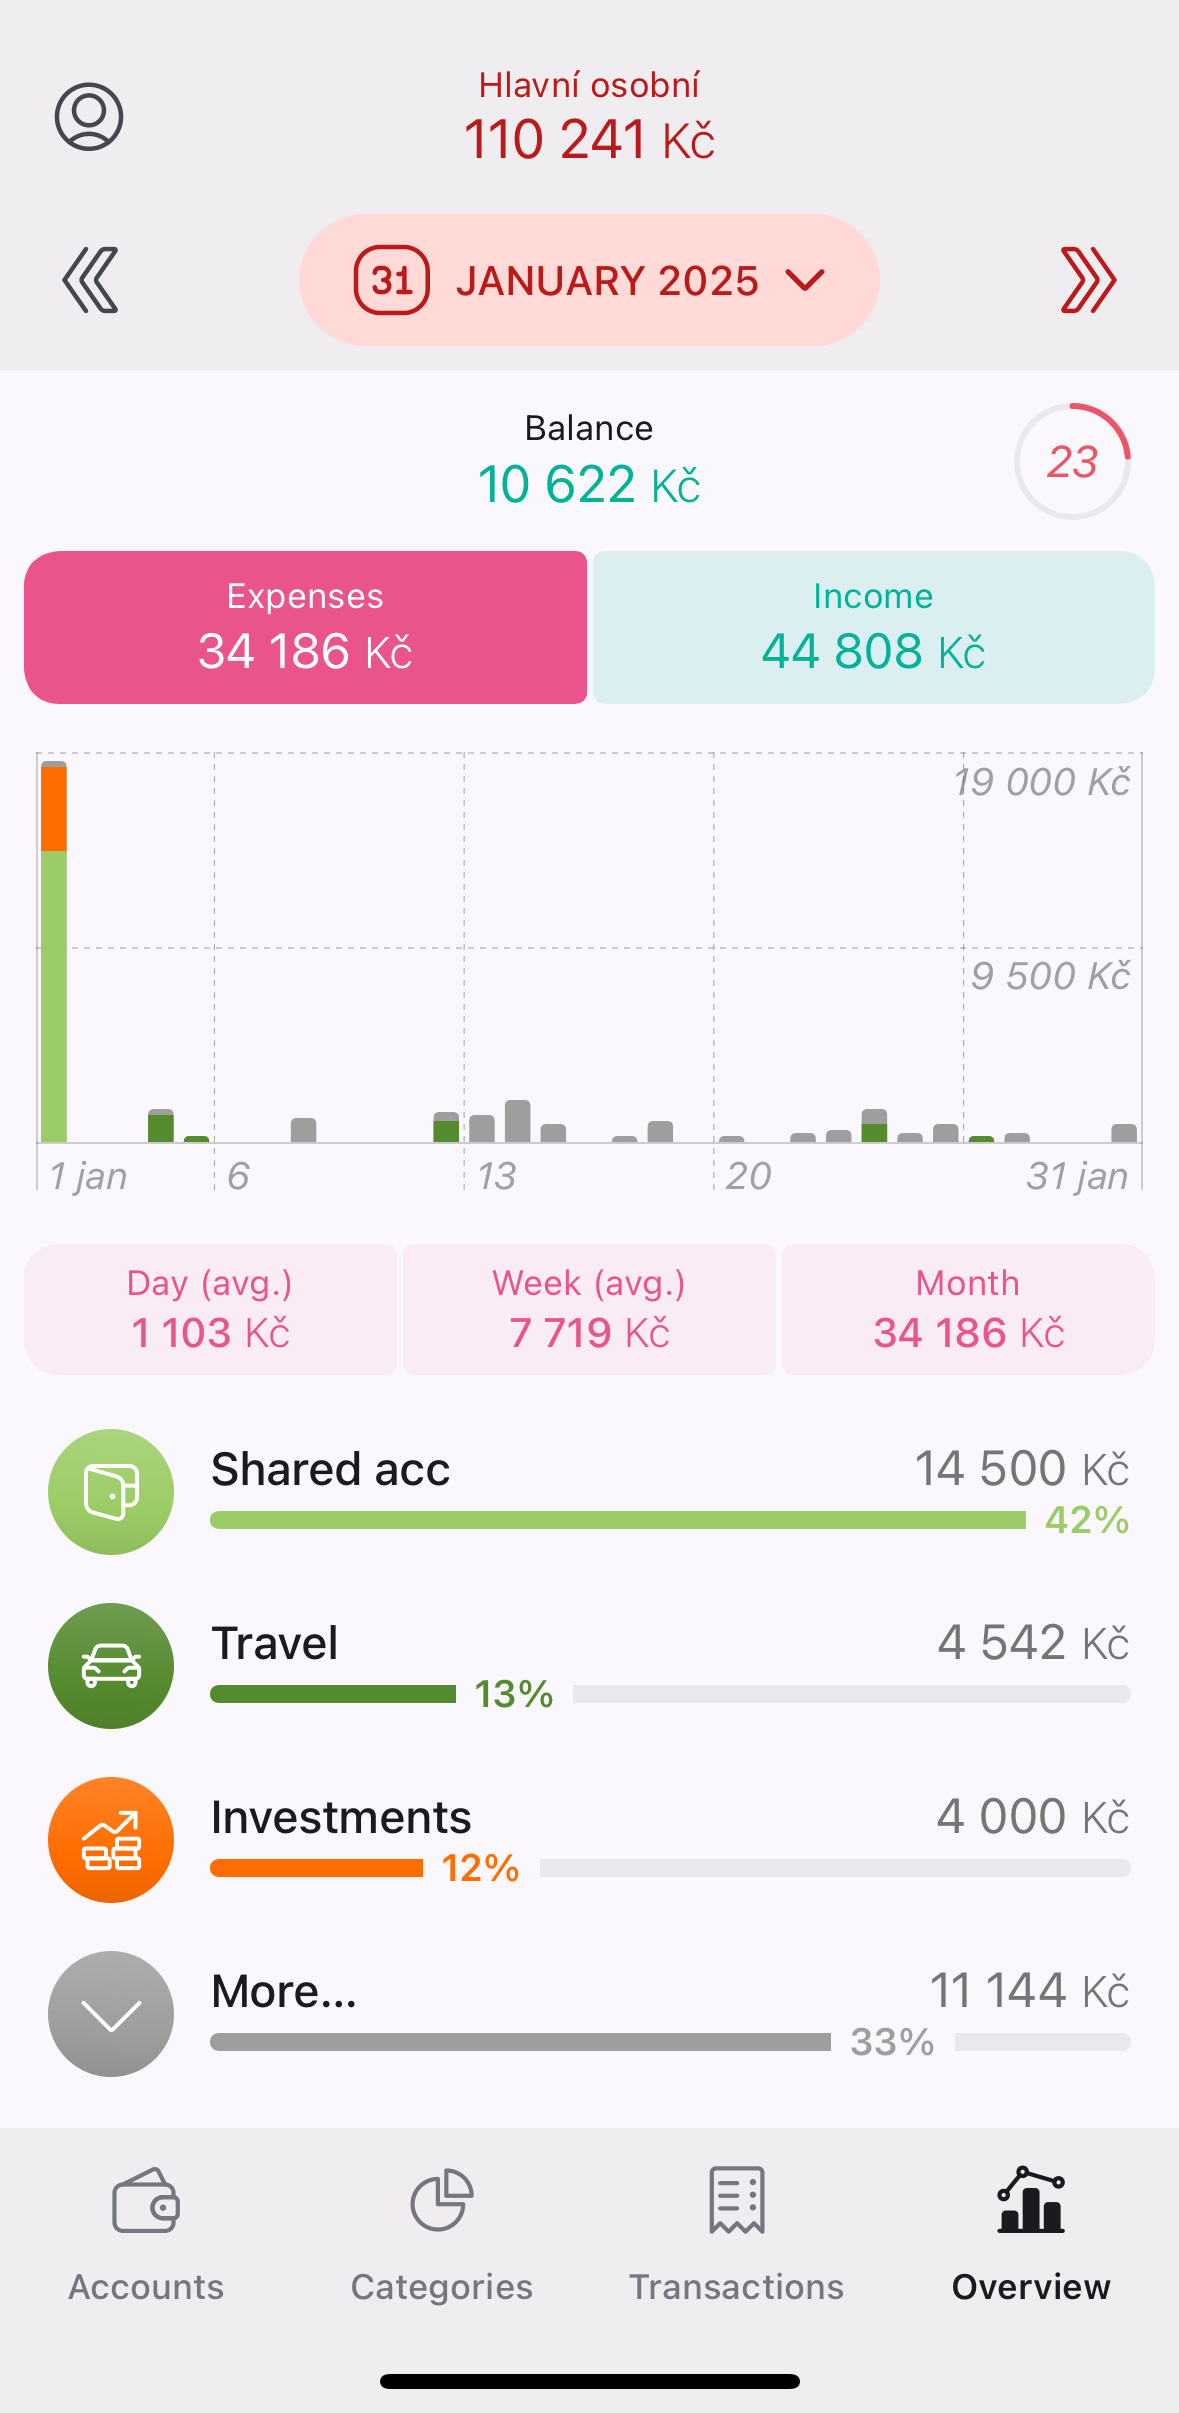
\includegraphics[width=0.35\textwidth]{images/onemoney1.PNG}
    \hspace{10px}
    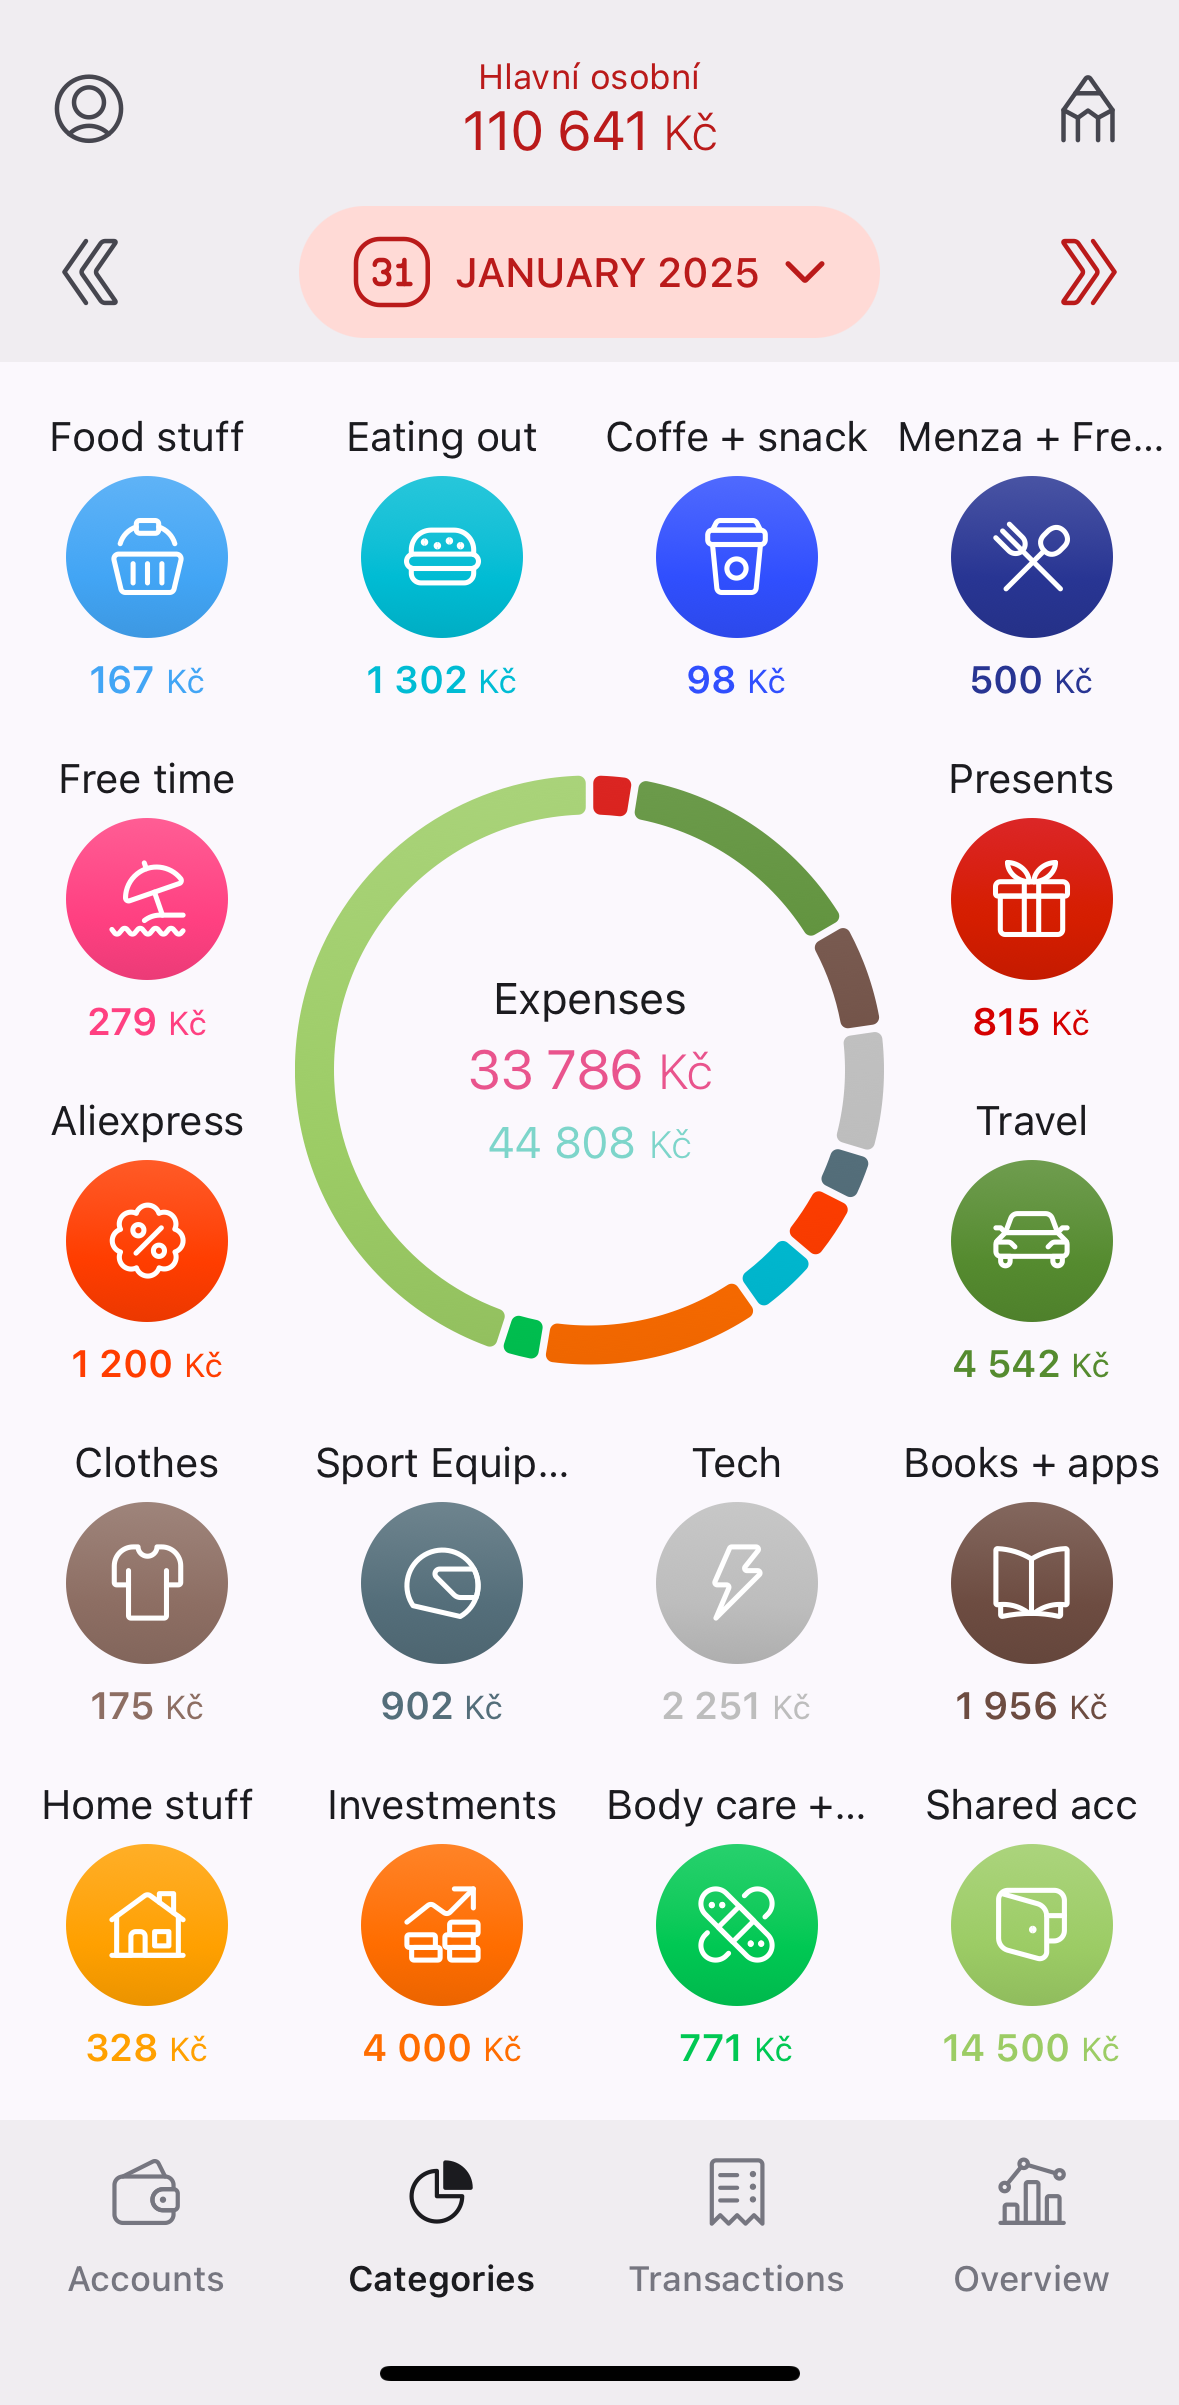
\includegraphics[width=0.35\textwidth]{images/onemoney2.PNG}
    \caption{Aplikace 1Money}
    \label{fig:1money}
\end{figure}

\subsection{Cashew}
Multiplatformní aplikace, založená na stejné technologii Flutter jako moje aplikace, se jmenuje Cashew \cite{cashew}. Implementuje komponenty ze systému Material Design (viz kapitola~\ref{sec:material-design}~\nameref{sec:material-design} a \hyperref[fig:cashew]{Obrázek \ref{fig:cashew}}), ale rozvržení obrazovky si autoři uspořádali podle sebe. Uživateli umožňuje široké možnosti nastavení z~hlediska vzhledu (barvy, fonty, typ ikon či formáty čísel). Umožňuje zálohování dat na Google disk i import z~CSV souborů. Podporuje funkci více účtů. Obsahuje i placenou verzi, které je primárně podporu pro vývojáře.

\begin{figure}
  \centering
    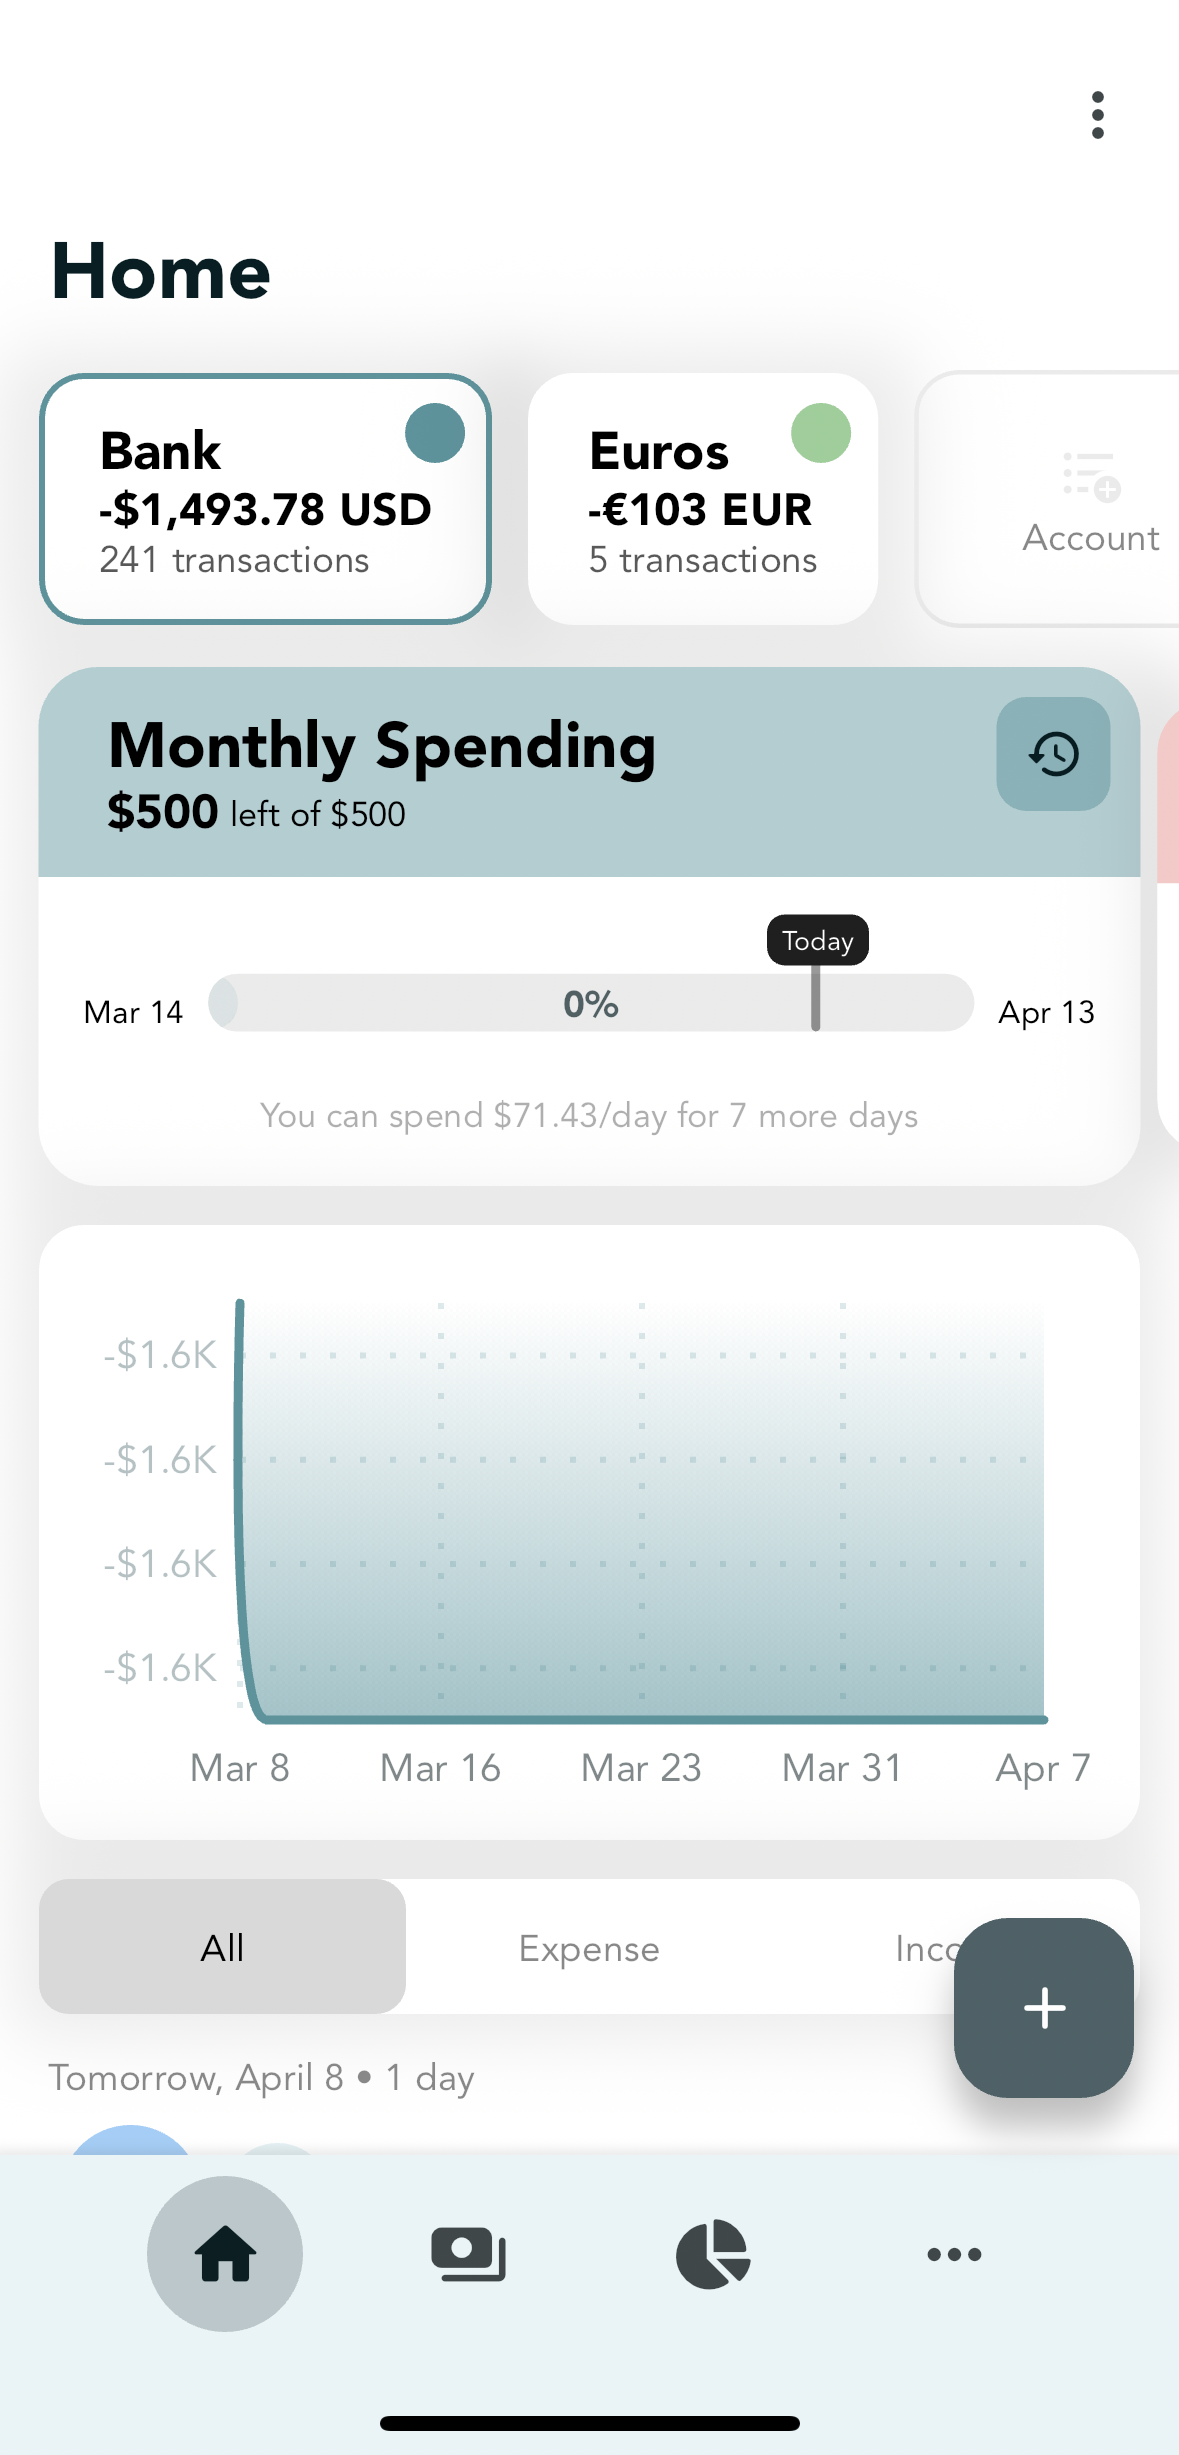
\includegraphics[width=0.35\textwidth]{images/cashew2.PNG}
    \hspace{10px}
    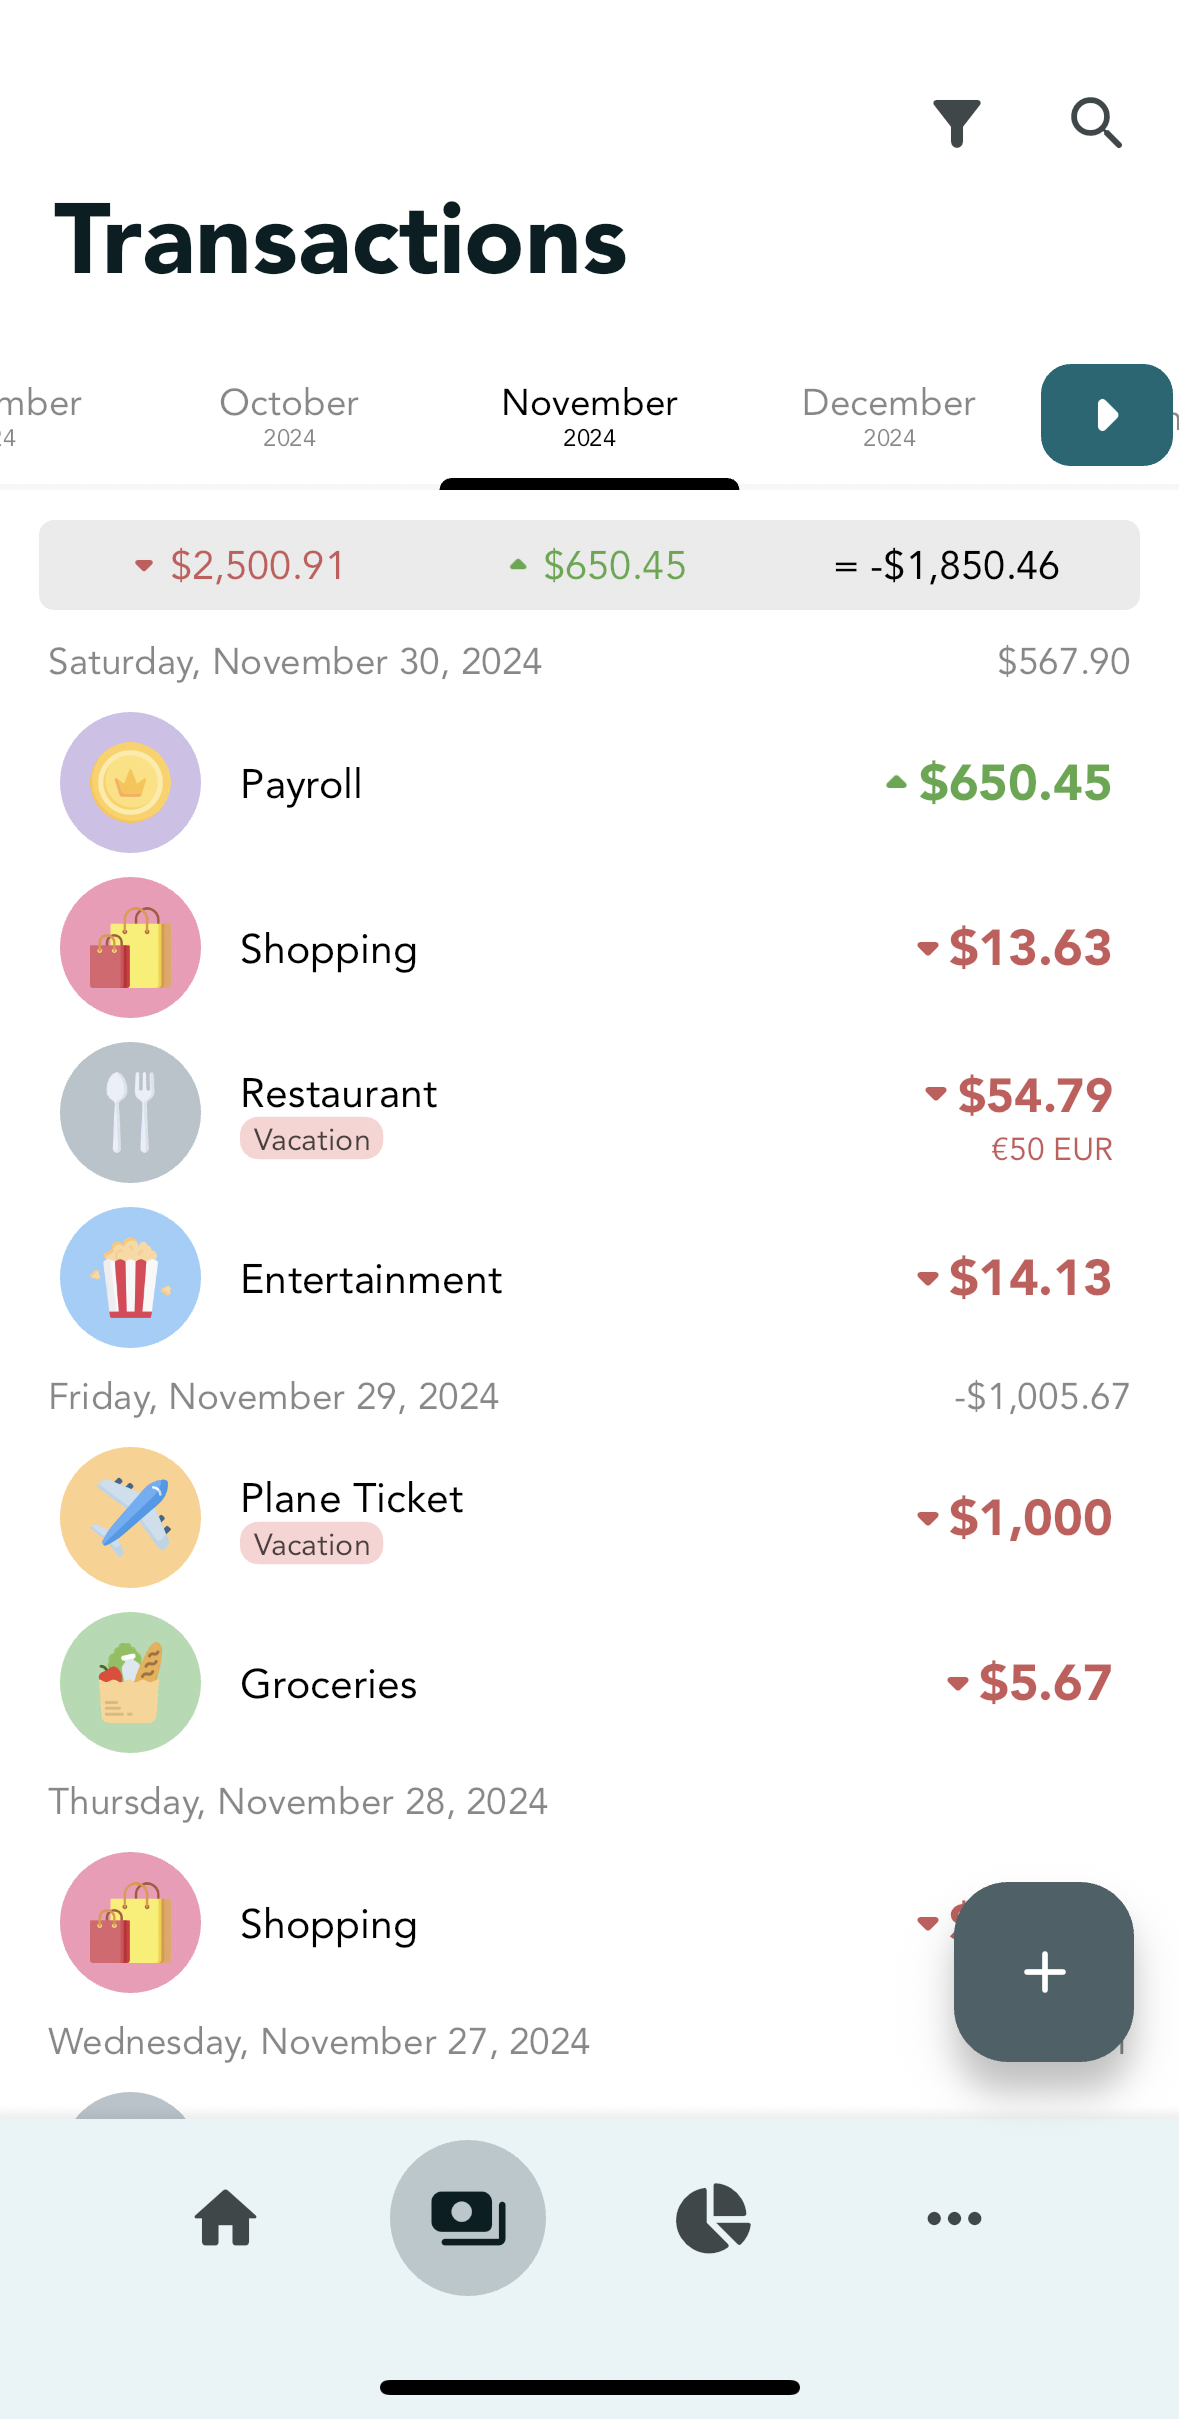
\includegraphics[width=0.35\textwidth]{images/cashew1.PNG}
  \caption{Aplikace Cashew}
  \label{fig:cashew}
\end{figure}

\subsection{Wallet}
Mobilní aplikace Wallet \cite{wallet} je dostupná na platformy Android i iOS. Za její stažení uživatel v~první fázi nezaplatí. Nabízí všechny základní funkce, co by uživatel očekával -- kategorie transakcí, podpora více měn, přidání poznámky. Z~hlediska analýzy a grafového zobrazení je na výběr jen velmi málo možností v~nepřehledném uspořádání (viz \hyperref[fig:wallet]{Obrázek \ref{fig:wallet}}). Ze zajímavých funkcionalit stojí za zmínku plánované transakce nebo automatická bankovní synchronizace (součást placené varianty).

\begin{figure}
  \centering
  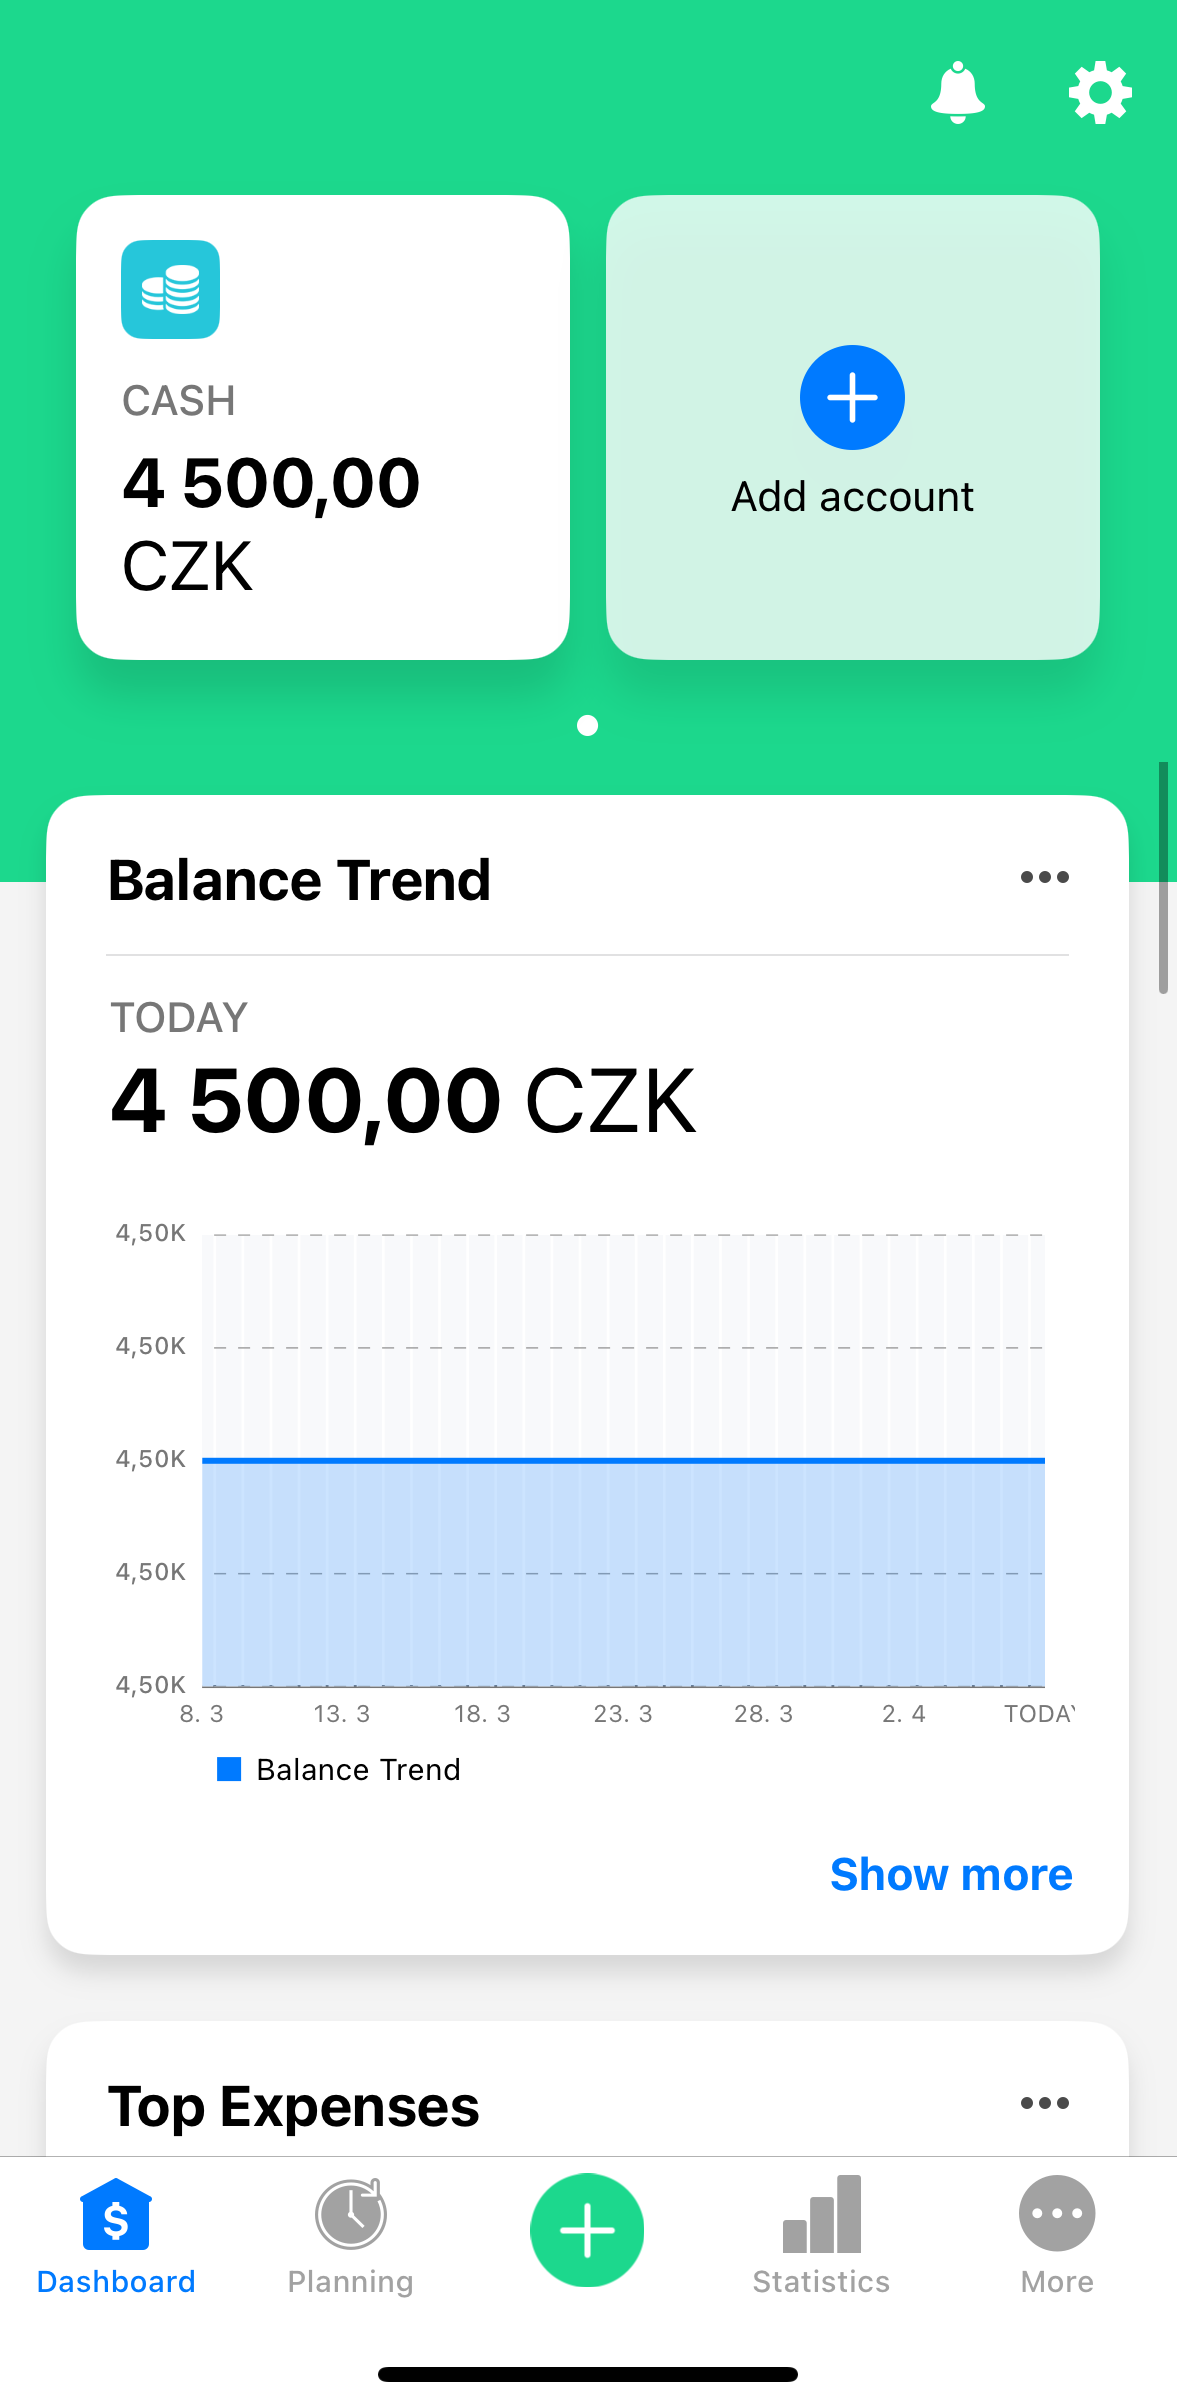
\includegraphics[width=0.35\textwidth]{images/wallet1.PNG}
    \hspace{10px}
    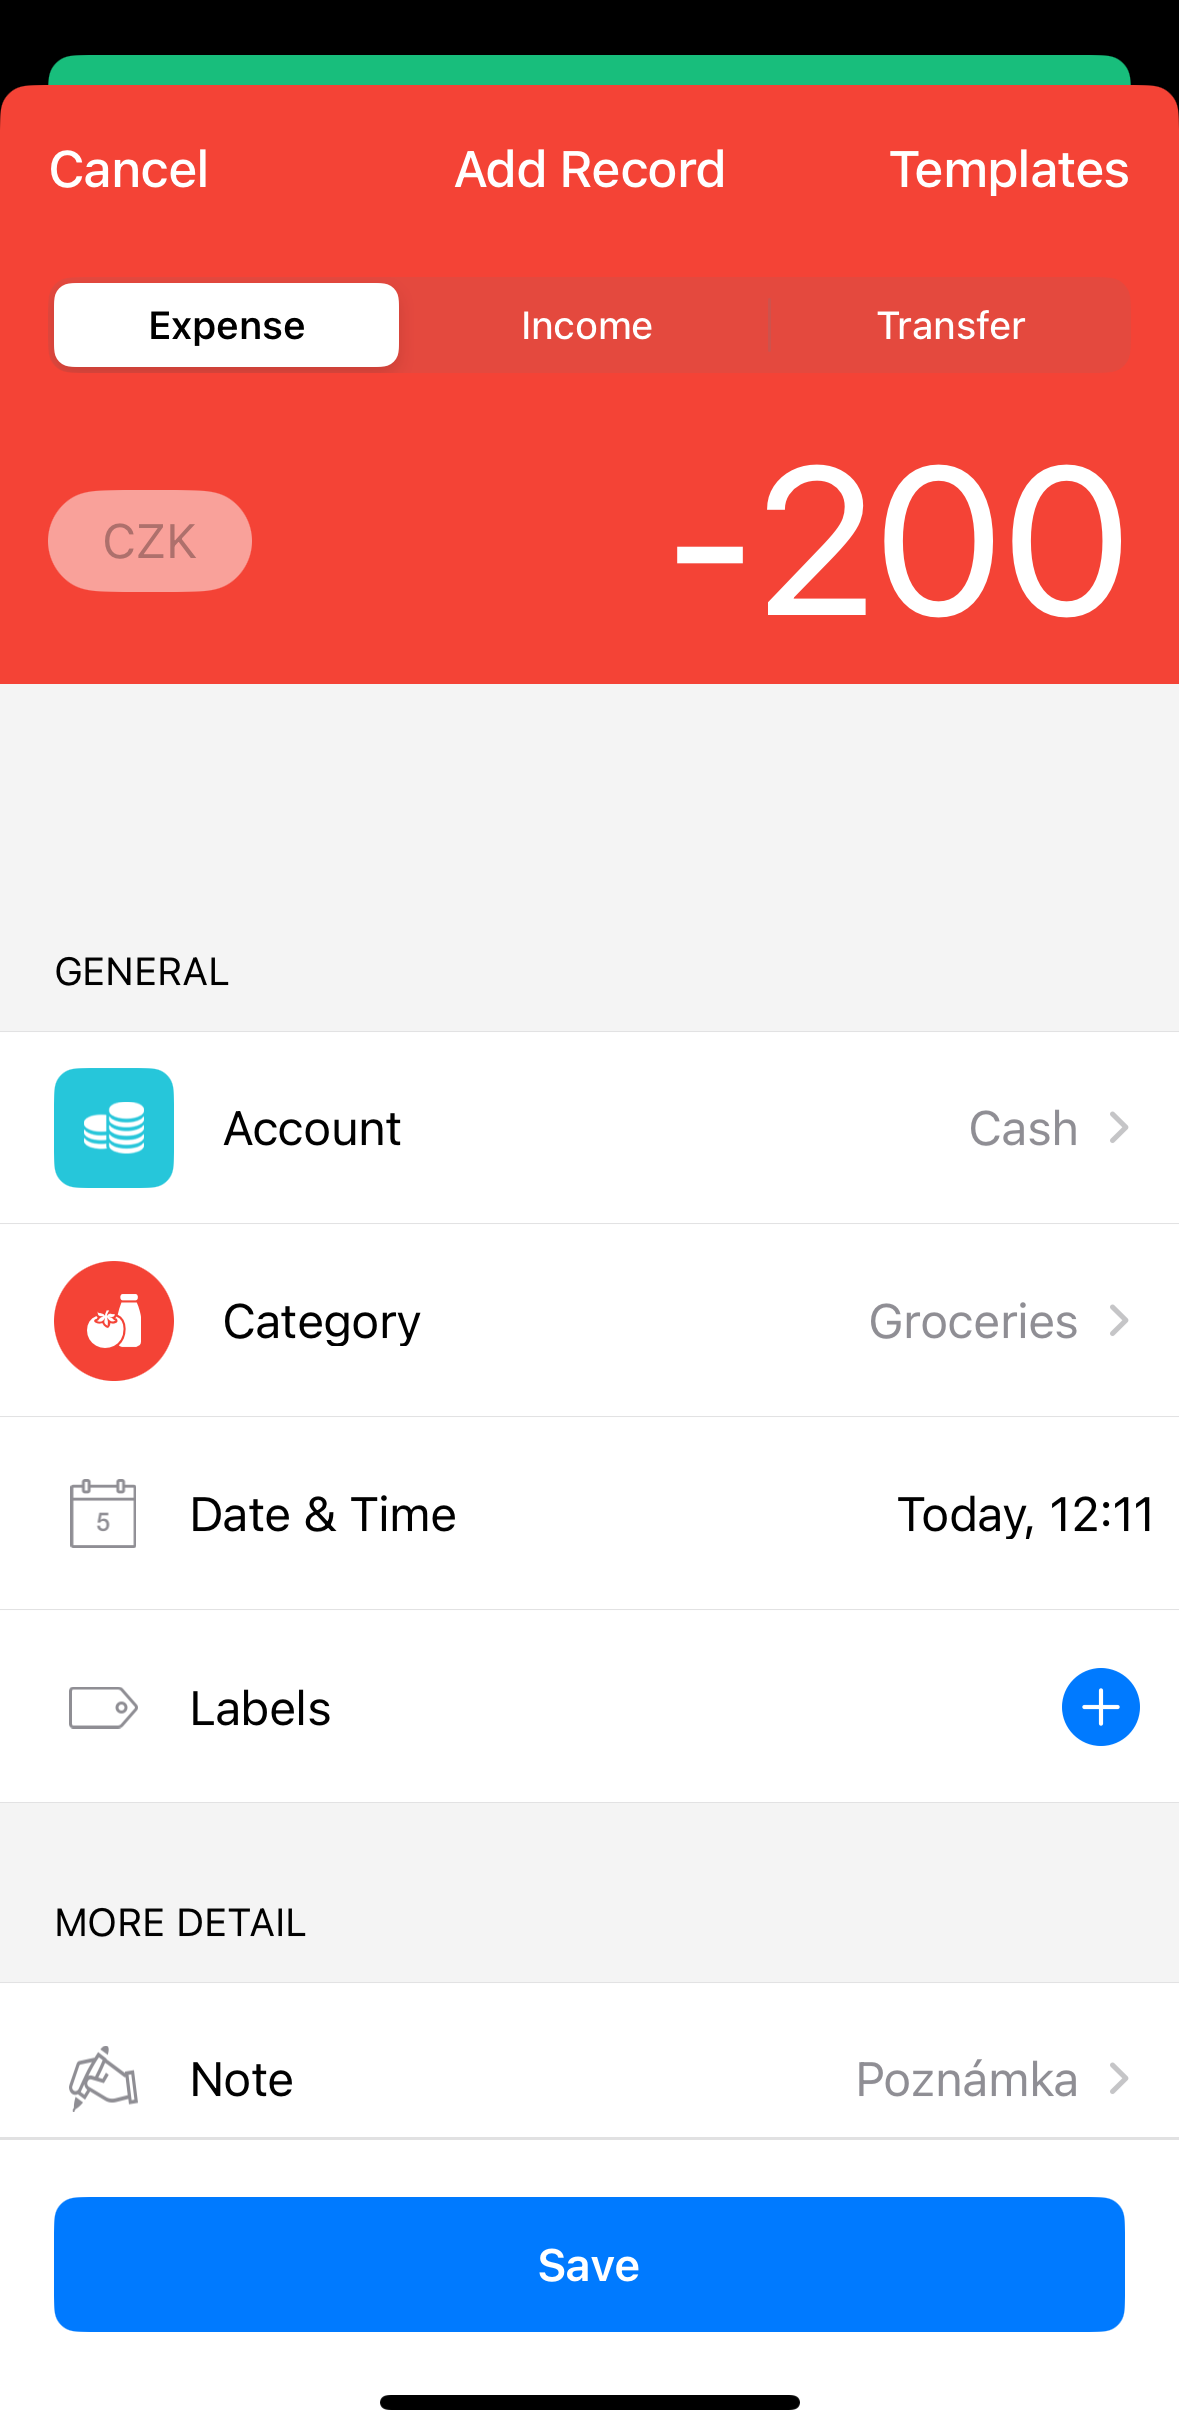
\includegraphics[width=0.35\textwidth]{images/wallet2.PNG}
  \caption{Aplikace Wallet}
  \label{fig:wallet}
\end{figure}

\subsection{Money Manager Ex}
Aplikace dostupná jak na mobilní telefony, tak především na desktopové zařízení \cite{money-manager}. Uživatelské rozhraní je na první pohled relativně přívětivé, i když místy obsahuje širokou škálu tlačítek a možností k~nastavení. Při prvním spuštění nevyžaduje žádné složité nastavení jak je vidět na \hyperref[fig:money-manager]{Obrázku \ref{fig:money-manager}}. Zde se mi velmi líbí velká nabídka grafů k~analýze údajů a možnost exportu do PDF formátu pro většinu obrazovek.

\begin{figure}
  \centering
  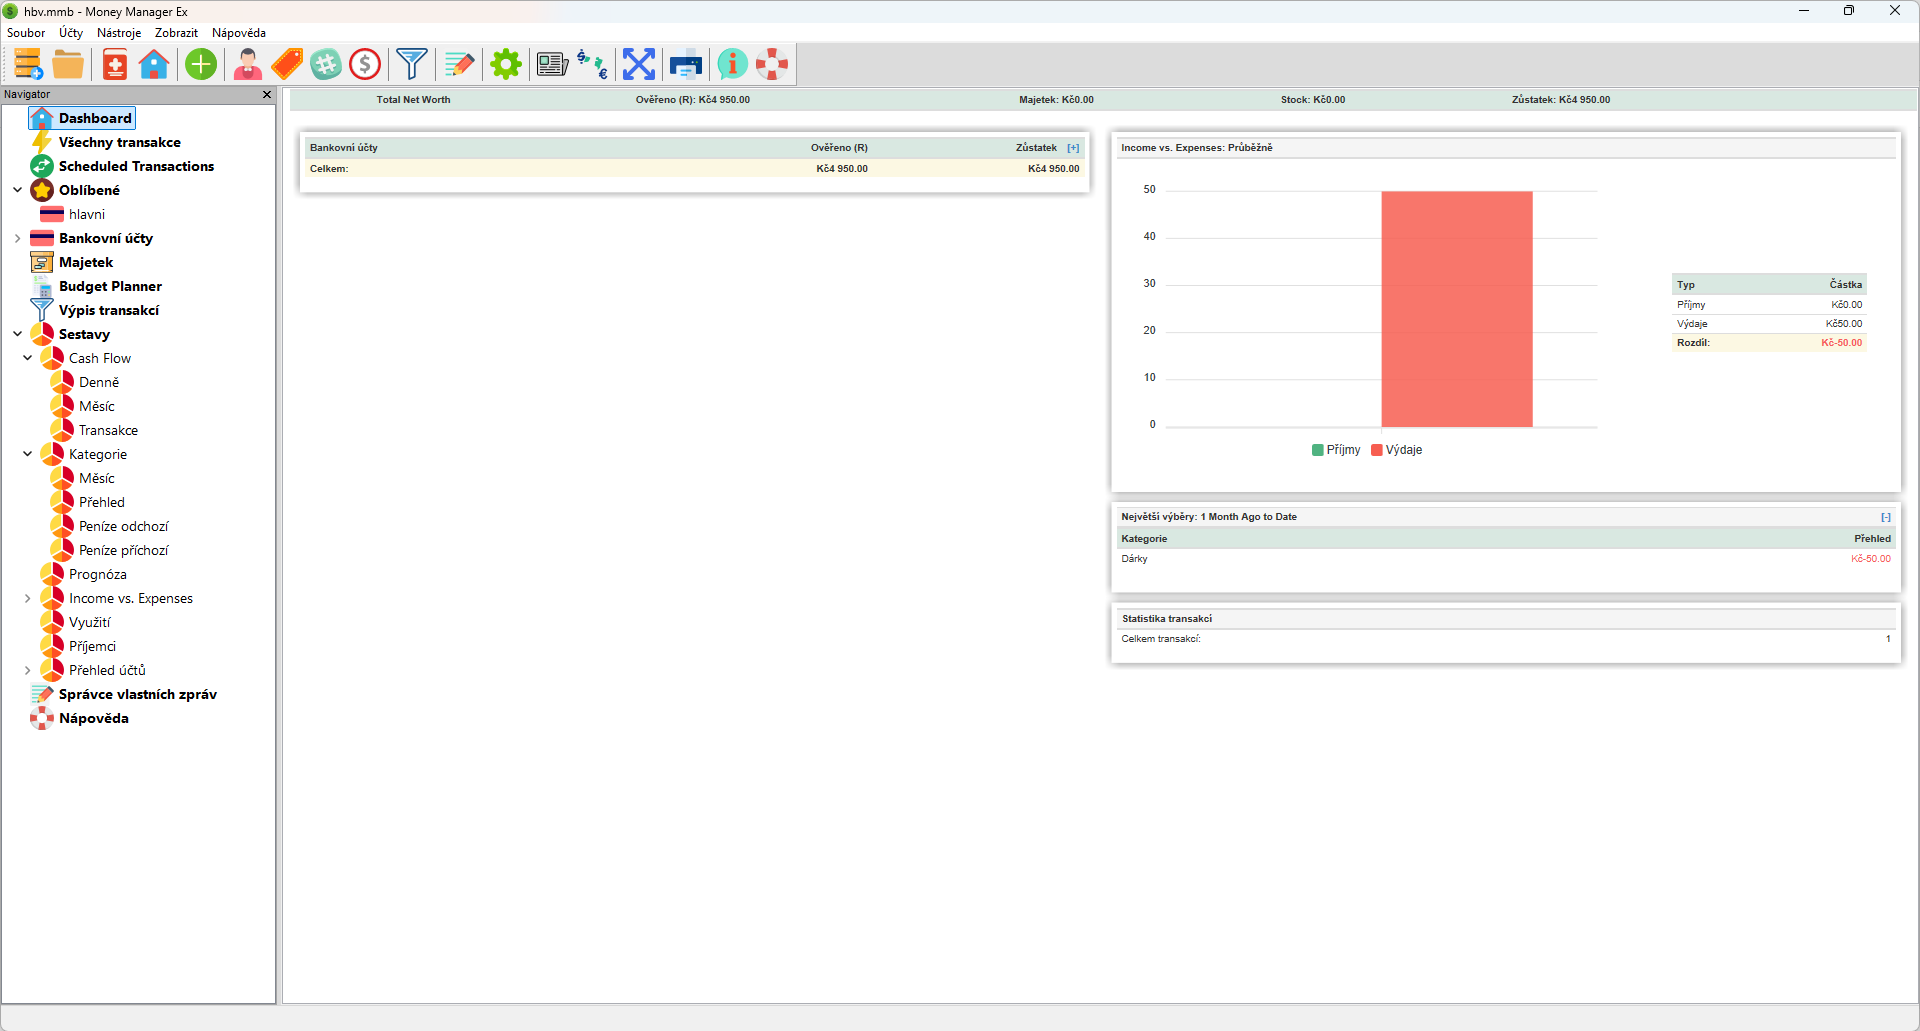
\includegraphics[width=1\textwidth]{images/manager-ex.png}
  \caption{Aplikace Money Manager Ex}
  \label{fig:money-manager}
\end{figure}

\subsection{Homebank}
Desktopová aplikace Homebank \cite{homebank} je dostupná na Windows, Linux i macOS. Z~hlediska uživatelského komfortu je oproti Money Manager Ex jednodušší na používání. Při prvotním nastavení sice člověk musí vhodně nakonfigurovat svůj účet, v~dalších fázích je už používání jednoduché. Centrem aplikace je obrazovka (viz \hyperref[fig:homebank]{Obrázek \ref{fig:homebank}}) se stavy účtu, přehledem transakcí a jednoduchými grafy. Všechny ostatní funkce se pak otevírají jako nové okno. Uživatelské rozhraní působí moderním a intuitivním dojmem.

\begin{figure}
  \centering
  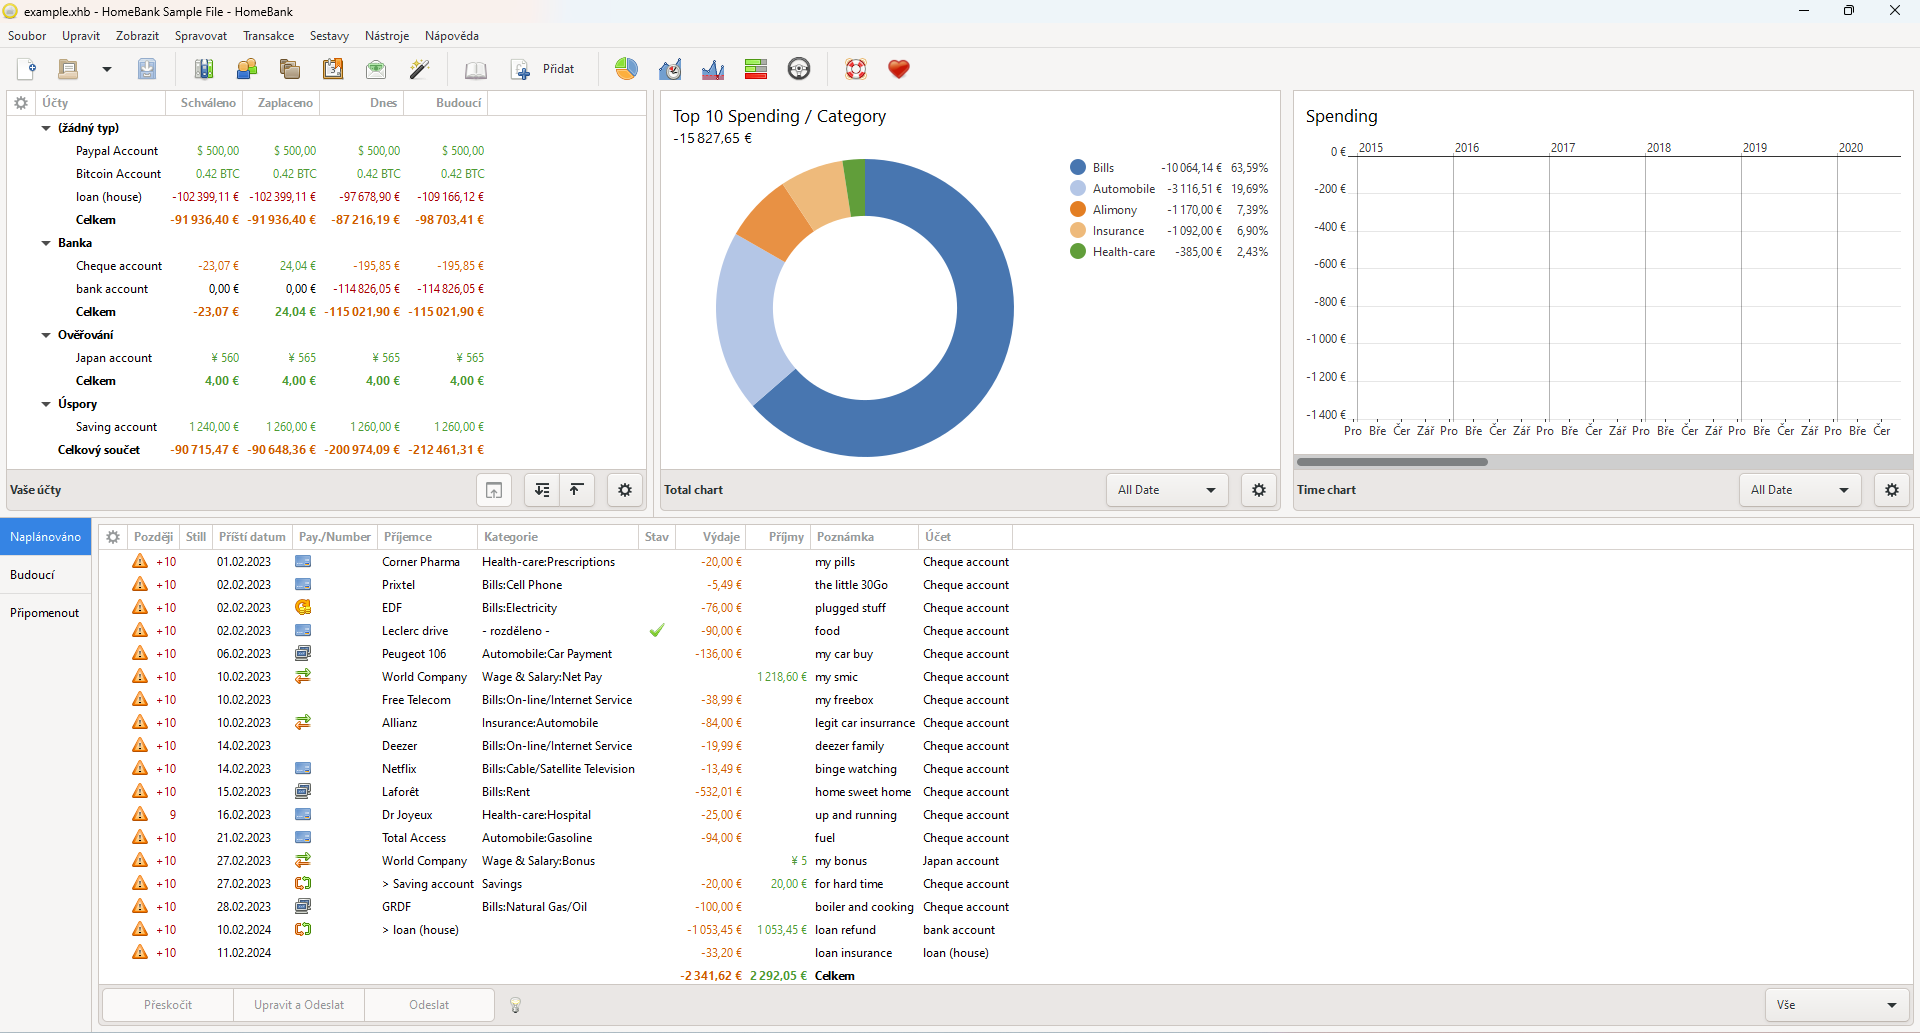
\includegraphics[width=1\textwidth]{images/homebank.png}
  \caption{Aplikace Homebank}
  \label{fig:homebank}
\end{figure}


Oproti existujícím aplikacím by mnou vytvořená aplikace měla nabídnout přívětivější uživatelské rozhraní a ulehčit první použití. Rád bych přinesl i lepší vizualizaci v~podobě grafů a zajímavých číselných údajů. V~neposlední řadě by měla být spustitelná na libovolné platformně, tak aby uživatel nebyl limitován například při změně mobilního telefonu.

\section{Použité technologie}

Hlavním požadavkem byl multiplatformní vývoj. K~této problematice existuje řada technologií \cite{jetbrains-crossplatform}, které však k~tvorbě aplikace přistupují odlišným způsobem. Mezi nejpopulárnější technologie vhodné na tuto práci se řadí \textit{React Native} a \textit{Flutter}. Jelikož jsem za dobu, co se věnuji programování nepřilnul k~webovým technologiím, na kterých primárně stojí React Native, zvolil jsem Flutter. Přispěl k~tomu fakt, že se více blíží klasickým objektově orientovaným jazykům a jednoduše implementuje systém Material Design, který rád v~uživatelském rozhraní vídám.

Aplikace je otestována a řádně funguje na mobilní platformě Android a jako desktopová Windows aplikace. Ze stejného kódu jde sestavit i aplikace na macOS a Linux. Tyto platformy jsem však netestoval a nemohu zaručit jejich bezproblémový chod.

\subsection{Dart}
Objektově orientovaný jazyk Dart \cite{dart} je vyvíjen společností Google. První verze byla zveřejněna 14. listopadu 2013, aktuální je verze 3. Jde o~typově bezpečný jazyk, podporující třídy, se syntaxí založenou na jazyku C. Může být kompilován do strojového kódu, jazyků JavaScript nebo WebAssembly. Taktéž je základem pro framework Flutter.

\kiinlinecode{}{;}
Je dodáván se širokou škálou základních knihoven, které umožňují obstarat běžný vývoj. Jako příklad uvádím knihovnu \kiinlinecode{}{;}{dart:async}, která umožňuje asynchronní programování za využití tříd jako \kiinlinecode{}{;}{Future} nebo knihovna \kiinlinecode{}{;}{dart:io} pro práci se souborovým systémem či HTTP protokolem.

Technologie jazyka Dart umožňují spustit kód dvěma způsoby. První z~nich je určen pro mobilní a desktopové aplikace. Dart obsahuje virtuální stroj s~JIT\footnote{Just in time} kompilací, který se používá především ve fázi vývoje. Tento způsob umožňuje tzv. inkrementální rekompilaci jejíž výhodou je funkcionalita \textit{hot reload} či nástroje \textit{DevTools} pro aktuální metriky ladění. Dále AOT\footnote{Ahead of time} kompilátor pro tvorbu strojového kódu, který se využívá při sestavování aplikace pro použití v~produkci. Druhý způsob se týká webové platformy, kde Dart umožňuje kód přeložit do jazyků JavaScript nebo WebAssembly. I~zde Dart využívá rozdílné techniky pro ladění kódu a následnou produkci. Oba tyto způsoby jsou stejné v~tom že potřebují \textit{běhové prostředí Dart}. Toto prostředí se stará o~správu paměti pomocí garbage collector, vynucení kontroly typů a správu vláken.

\begin{kicode}{}{}{Ukázka kódu v~jazyce Dart}
class Point {
  final double x;
  final double y;

  const Point(this.x, this.y);

  bool get isInsideUnitCircle => x * x + y * y <= 1;
}
\end{kicode}

\subsection{Flutter}
Open source framework Flutter \cite{flutter} slouží pro tvorbu uživatelských rozhraní. Využívá jazyk Dart a je také vyvíjený společností Google. Poprvé zveřejněn byl v~květnu 2017. Google sám ho využívá v~aplikacích jako je Google Play nebo Google Earth \cite{flutter-showcase}. Mezi nejznámější aplikace třetích stran používajících Flutter patří Alibaba nebo hra PUBG Mobile \cite{flutter-showcase}.

Používá vlastní vykreslovací jádro, které pixely přímo vykresluje na obrazovku. Toto je podstatný rozdíl oproti řadě jiných frameworků, které se spoléhají na vykreslovací jádro dané platformy. Tento přístup umožňuje mít identicky vypadající uživatelské rozhraní napříč všemi podporovanými platformami.

Základní komponentou je \textit{widget}. Ten se může skládat z~dalších widgetů a vytvářet tak stromovou strukturu. Celé uživatelské rozhraní je poskládáno widgetů. Flutter poskytuje dva typy předdefinovaných widgetů podle dvou designových systémů -- Material Design (viz kapitola~\ref{sec:material-design}~\nameref{sec:material-design}) widgety a Cupertino widgety. Přestože oba mají svoji primární platformu, Flutter je umožňuje používat libovolně. Programátor si samozřejmě může definovat widgety vlastní.

Pro rozložení prvků na stránce (vytvoření \textit{layout}) se taktéž používají widgety, přestože nejsou při zobrazení viditelné. Základními widgety pro tvorbu layoutu jsou \kiinlinecode{}{;}{Row}, \kiinlinecode{}{;}{Column} a \kiinlinecode{}{;}{Container}. Pomocí \kiinlinecode{}{;}{Container} můžeme ostatním widgetům přidávat odsazení, ohraničení, transformaci atd. Tyto widgety slouží pro specifickou či nízkoúrovňovou tvorbu layoutu. Můžeme využít i specializované widgety jako \kiinlinecode{}{;}{GridView} pro tvorbu mřížky nebo \kiinlinecode{}{;}{ListView} pro rolovatelný seznam. Nejvíce specifické widgety jako \kiinlinecode{}{;}{BottomNavigationBar} či \kiinlinecode{}{;}{AppBar} zajistí dodržení pravidel stanovených systémem Material Design a umožní programátorovi velmi jednoduchou implementaci.

\subsection{Material Design} \label{sec:material-design}
V~březnu 2025 je Material Design verze 3 \cite{m3} nejnovějším open source designový systém od společnosti Google. Systémem v~tomto případě mám na mysli soubor pravidel pro uživatelské rozhraní, konkrétní komponenty i barevné provedení. Všechny tyto prvky jsou vytvořeny zkušenými designéry s~respektem pro psychologický vliv uživatelského rozhraní na člověka.

Označení verze 3 napovídá, že v~minulosti již proběhly aktualizace tohoto systému. Tento krok dává smysl vzhledem k~vyvíjejícím se trendům v~oblasti designu. Aktualizace mohl uživatel pozorovat v~operačním systému Android nebo v~aplikacích od Google, jelikož Google tento systém používá téměř všude.

Použití tohoto systému má ve Flutteru řadu výhod. Především většina widgetů ze systému Material Design je již implementována a použití programátorem je velmi jednoduché. Programátor nemusí často řešit rozmístění jednotlivých prvků v~konkrétní komponentě ani správnou adaptaci na velikost zařízení. Běžnou součástí aplikací jsou ikony. Ikony z~Material Designu jsou ve Flutteru k~přímému použití bez specifického nastavení. Programátor nemusí řešit žádné externí SVG soubory. Stejně to platí i pro použití fontů písem.

\subsection{SQLite}
SQLite \cite{sqlite} je velmi jednoduchá a rychlá relační databáze, která je uložena v~jediném souboru. Vývoj SQLite byl zahájen v~roce 2000. Obvykle jsou všechny potřebné závislosti již zabudovány v~zařízeních, ať už jde o~mobilní telefony nebo desktopové operační systémy. Je zdarma k~užití pro libovolné účely. Přesto poskytuje plnohodnotnou SQL implementaci. Zajímavostí je, že onen soubor je multiplatformní. Nevadí mu přenos mezi 32bitovými a 64bitovými systémy nebo architekturami big-endian a little-endian.

\subsection{Balíčky}

Přestože balíčky tvoří závislosti projektu na ostatních okolnostech a programátor se musí spoléhat na jiné programátory, že je budou udržovat aktuální, je nemožné se jim v~dnešním době vyhnout. Dart a Flutter má na výběr z~široké veřejné knihovny balíčků. Balíčky je nutné do projektu importovat. Celý jejich seznam je dostupný v~souboru \kiinlinecode{}{;}{pubspec.yaml}. Přidání balíčku do projektu se provádí zapsáním do souboru \kiinlinecode{}{;}{pubspec.yaml} a spuštěním příkazu \kiinlinecode{}{;}{flutter pub get} nebo rovnou příkazem \kiinlinecode{}{;}{}\kiinlinecode{}{;}{flutter pub add <název_balíčku>}.

\begin{itemize}
  \item \textbf{Drift} \cite{drift} je balíček poskytující rozhraní pro práci s~SQLite databází. Jeho velkou výhodou oproti ostatním implementacím SQLite pro Dart je možnost multiplatformnosti. Funguje na všech platformách od Androidu přes Windows až po webové rozhraní (na rozdíl od knihovny sqflite, která je zmíněna v~oficiálním návodu). Dále poskytuje velmi jednoduché API pro vytváření dotazů nad databází bez použití jazyka SQL. Programátor vytváří strukturu databáze v~jednom souboru, na jehož základě si Drift generuje interní soubory.
  \item \textbf{GoRouter} \cite{gorouter} je deklarativní balíček pro organizaci navigace v~rámci aplikace (tzv. \textit{routování}). Funguje na principu URL adres. Umožňuje v~adrese předávat parametry, zajistit přesměrování na základě práv uživatele či použití \textit{vnitřních navigátorů} nejčastěji pro navigaci, která zůstává neustále viditelná skrz více obrazovek. Pro přechody umožňuje nastavit vlastní libovolné animace. Autory jsou přímo oficiální vývojáři frameworku Flutter.
  \item \textbf{Skeletonizer} \cite{skeletonizer} zjednodušeným způsobem poskytuje funkcionalitu označovanou jako \textit{skeleton loading}. Používá se při načítání obsahu na stránce a zobrazuje hrubý náhled rozložení prvků na stránce (znázorněno  na \hyperref[fig:skeleton]{obrázku \ref{fig:skeleton}}). Vše je doplněno vhodnou animací, aby uživatel ihned poznal, že se obrazovka načítá. Zjednodušení použitím tohoto balíčku spočívá v~tom, že programátorovi stačí již definovaný widget \uv{obalit} widgetem \kiinlinecode{}{;}{Skeletonizer} z~tohoto balíčku a o~zbytek práce se postará balíček.
  
  \begin{figure}
  	\centering
  	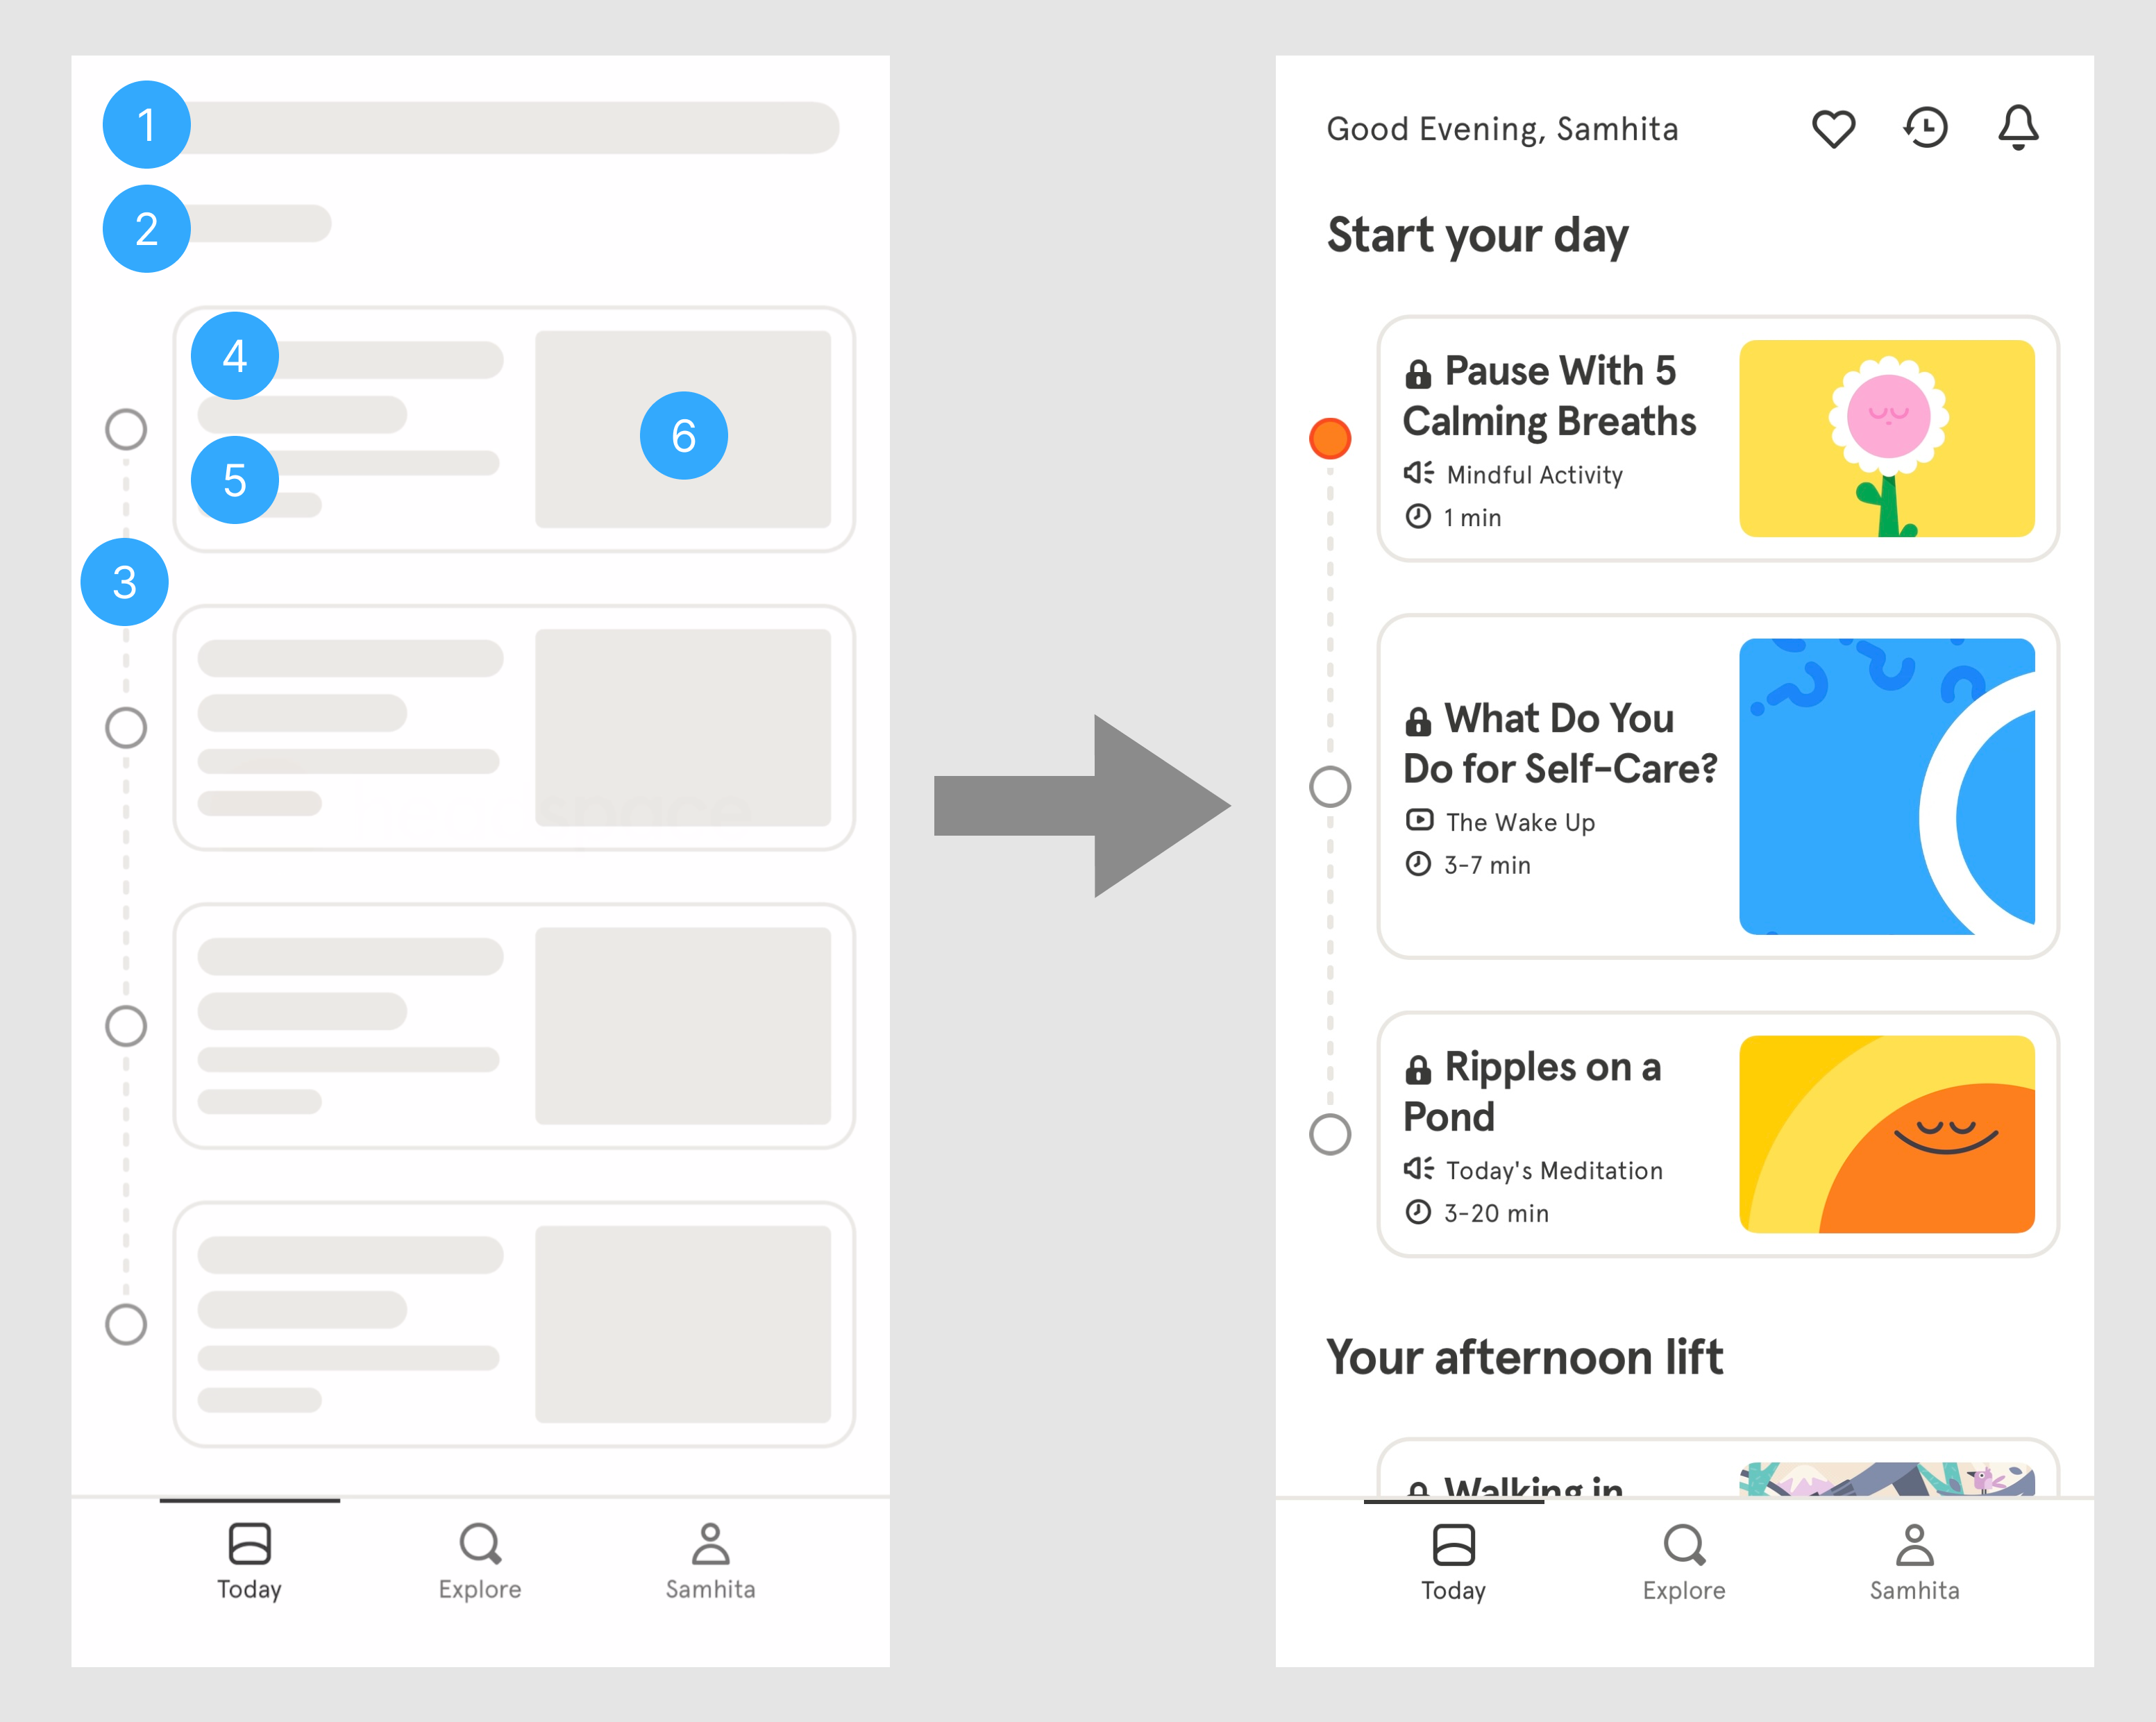
\includegraphics[scale=0.1]{images/skeletonizer.png}
  	\caption{Skeleton loading a načtená obrazovka -- převzato z~\cite{skeleton}}
    \label{fig:skeleton}
  \end{figure}
  
  \item \textbf{Another Flushbar} \cite{flushbar} poskytuje vylepšenou komponentu \kiinlinecode{}{;}{Snackbar} ze systému Material Design. Účelem komponenty je krátce informovat uživatele o~akci, která byla právě provedena (například akce úspěšného exportu transakcí je znázorněna na \hyperref[fig:flushbar]{obrázku \ref{fig:flushbar}}). Obvykle se objevuje ve spodní části obrazovky. Vylepšení spočítá v~možnosti většího přizpůsobením - přidání ikony, změna barvy či animace a libovolné umístění. Já tento balíček preferoval i z~důvodu správného zobrazování při otevřeném dialogovém okně.

  \begin{figure}
    \centering
    
\includegraphics[width=0.5\textwidth]{images/flushbar.pdf}
    \caption{Komponenta Flushbar}
    \label{fig:flushbar}
  \end{figure}
      
  \item \textbf{Syncfusion Flutter Charts} \cite{syncfusion-charts} je rozsáhlý balíček pro tvorbu grafů. Umožňuje vytvářet všechny druhy grafů -- sloupcové, spojnicové, prstencové a další (autoři uvádí více než 30 druhů). Grafy lze dále přizpůsobovat -- výběr animace, úprav jednotek na osách, výběr barev, možnost zobrazit legendu či podrobné informace daného bodu v~grafu po přejetí myší. Přes širokou škálu úprav je základní použití velmi jednoduché. Bonusem je podrobná dokumentace s~ukázkami všech typů grafů a jejich zdrojových kódů.
  \item \textbf{File Picker} \cite{file-picker} dává programátorovi možnost využít nativní průzkumník souborů k~výběru složky nebo konkrétních souborů pro jejich další zpracování v~aplikaci. Je možnost soubory filtrovat či umožnit výběr více z~nich najednou. Základní funkcionalitu poskytuje na libovolné platformně s~velmi jednoduchou implementací. V~mém případě jsem ho použil pro výběr složky, kam si uživatel chce uložit exportované soubory. 
\end{itemize}


\section{Programátorská příručka}

Multiplatformní vývoj přináší jistá specifika (nutnost zvolit vhodné technologie, případnou optimalizaci zobrazení či zúžený výběr knihoven). Z~hlediska architektury či samotného procesu programování je postup z~většiny totožný jako u~programování pro jednu platformu. Zvolená technologie často sama navádí k~použití vhodných prvků.

Mnou navržené a vytvořené aplikaci jsem dal název Budget Buddy. Je určena pro mobilní telefony, tablety i desktopová zařízení. Testování probíhalo na operačních systémech Android, iOS a Windows. Pro ostatní operační systémy není zaručena plná funkcionalita, i když z~podstaty frameworku by se tak stát nemělo.

Pro vývoj aplikace jsem použil textový editor Visual Studio Code s~řadou rozšíření. Část práce specifické pro platformu Android jsem realizoval v~prostředí Android Studio. Především se jednalo o~úlohy typu aktualizace Software Developement Kit či migrace na novější verzi Kotlin gradle, kde Android Studio poskytuje jednodušší rozhraní a programátora provede celým procesem.

\subsection{Architektura aplikace}
Pro multiplatformní vývoj neexistuje doporučená architektura už z~podstaty věci širokého záběru různých zařízení. Je možné se držet dlouho známých architektur, které se používají v~různých systémech (\textit{Model-View-Controller} či \textit{Mode-View-ViewModel}) nebo se řídit podle zvyklostí daného frameworku (ve Flutteru se jedná například o~\textit{Bloc} \cite{bloc}). Já se ve své aplikaci držel architektury Model-View-Viewmodel, jelikož s~ní mám z~minulosti zkušenosti a~pro moji malou aplikaci je plně dostačující. 

Model-View-ViewModel (zkráceně MVVM) je architektura, která odděluje v~aplikaci uživatelské rozhraní, logiku a datovou část \cite{mvvm}. Ve framworku Flutter je velmi dobře podporována, jednak z~hlediska komponent frameworku, tak i oficiální dokumentace na architekturu odkazuje jako vhodný příklad návrhu aplikace. Rozdělení aplikace je do následujících tří detailněji popsaných celků.
\begin{itemize}
  \item \textbf{Model} je částí zapouzdřující data, se kterými aplikace pracuje. Udává strukturu poskytovaných dat i metody pro jejich získání objekty ve Viewmodel.
  \item \textbf{View} je zodpovědné za strukturu a zobrazení uživatelského rozhraní. Neměl by obsahovat žádnou logiku aplikace. Vstupy které přijme od uživatele předává ke zpracování na ViewModel. 
  \item \textbf{ViewModel} je prostředníkem mezi View a Model. Do View poskytuje data a případně je upraví do vhodného formátu pro zobrazení. Reaguje na zprávy od View, které představují vstupy uživatele. Vlákno pro uživatelské rozhraní by neměl blokovat, zlepší se tím uživatelský zážitek.
\end{itemize}

V~mé konkrétní implementaci je kód strukturován do složek podle MVVM architektury -- \kiinlinecode{}{;}{model}, \kiinlinecode{}{;}{view} a \kiinlinecode{}{;}{view_model}. Ve \kiinlinecode{}{;}{view} je jemnější rozdělení na obrazovky \kiinlinecode{}{;}{screens} a jednotlivé widgety \kiinlinecode{}{;}{widgets}. Dále je v~projektu i složka \kiinlinecode{}{;}{data} pro databázi, složka \kiinlinecode{}{;}{utils} pro jednoduché funkce používané skrz projektem (převod kódu ikony na Ikonu, zkrášlení číselného formátu a další) a složka \kiinlinecode{}{;}{theme} spravuje vizuální téma aplikace.

\subsection{Uchovávání stavu}
Uchování stavu jednotlivých obrazovek a jiných prvků je velmi důležité pro uživatelský komfort. Běžně se uživatel překlikne nebo přeskakuje mezi obrazovkami a není žádoucí, aby po každé byla obrazovka ve výchozím stavu (např. aby bylo nutné opět scrollovat v~seznamu). Použití GoRouter za programátora řeší i tento problém. Není nutné nic nastavovat a stačí řídit se dokumentací GoRouter. Po zavedení do aplikace již uchování stavů funguje přesně tak, jak je pro uživatelský komfort vhodné. V~první řade bylo nutné vytvořit aplikaci konstruktorem ~\kiinlinecode{}{;}{MaterialApp.router}. Do parametru \kiinlinecode{}{;}{_router} jsem vložil konfiguraci GoRouter (viz kód \ref{gorouter-code}). V~konfiguraci je uvedena cesta a obrazovka, která se při jejím zadání zobrazí.

\begin{kicode}{csharp}{gorouter-code}{Ukázka použití GoRouter}
  // GoRouter konfigurace
  final _router = GoRouter(
    routes: [
      GoRoute(
        path: '/',
        builder: (context, state) => HomeScreen(),
      ),
    ],
  );

  // konstruktor aplikace
  class MyApp extends StatelessWidget {
    @override
    Widget build(BuildContext context) {
      return MaterialApp.router(
        routerConfig: _router,
      );
    }
  }
\end{kicode}

\subsection{Implementace responzivního designu}
Responzivní design má zajistit, že aplikace se bude vhodně zobrazovat na libovolně velkém zařízení. Vyskytuje se především u~webových technologií z~důvodu běžného používání na různých typech zařízení. Stejná problematika je u~multiplatformních aplikací.

Podle velikosti obrazovky je nutné vhodně zvolit z~určitých komponent, které slouží pro stejný účel, ale jsou jinak zobrazené. V~této aplikaci se jedná například o~navigaci. Pro menší obrazovky jsem použil navigation bar, pro větší navigation rail, případně navigation drawer (viz \hyperref[fig:navigation]{Obrázek \ref{fig:navigation}}). Dále je nutné vhodně zobrazit komponenty v~hlavním těle obrazovky. Řazení komponent na menším zařízení jsem zvolil pod sebe do sloupce, na větším naopak vedle sebe v~řádku (viz obrázek grafy v~mé appce). Je dostupná i komponenta \kiinlinecode{}{;}{GridView} vytvářející tabulku. Avšak není vhodná pro tvorbu layoutu. Material Design poskytuje i~speciální kanonické rozložení (viz \hyperref[fig:canonical-layout]{Obrázek \ref{fig:canonical-layout}}), které je vhodné ve spojení se zobrazením seznamu. V~této aplikaci by bylo vhodné pro obrazovku transakcí. Implementace pro Flutter zatím není dostupná, tudíž není možné ho použít. Dialogová okna jsem podle doporučení pro menší zařízení zvolil celoobrazovková, zatímco na větších jsou plovoucí (viz obrázek dialog okno moje).

Flutter poskytuje komponenty vhodné pro responzivní design, ale na programátorovi je ponecháno kdy jaké zvolí, včetně celé implementace. Zatím není dostupná žádná komponenta pro tvorbu responzivního rozložení, které by umožnila v~jediném kódu pro uživatelské rozhraní rozhodnout do jakého widgetu kód \uv{obalit}.

\begin{figure}
  \centering 
  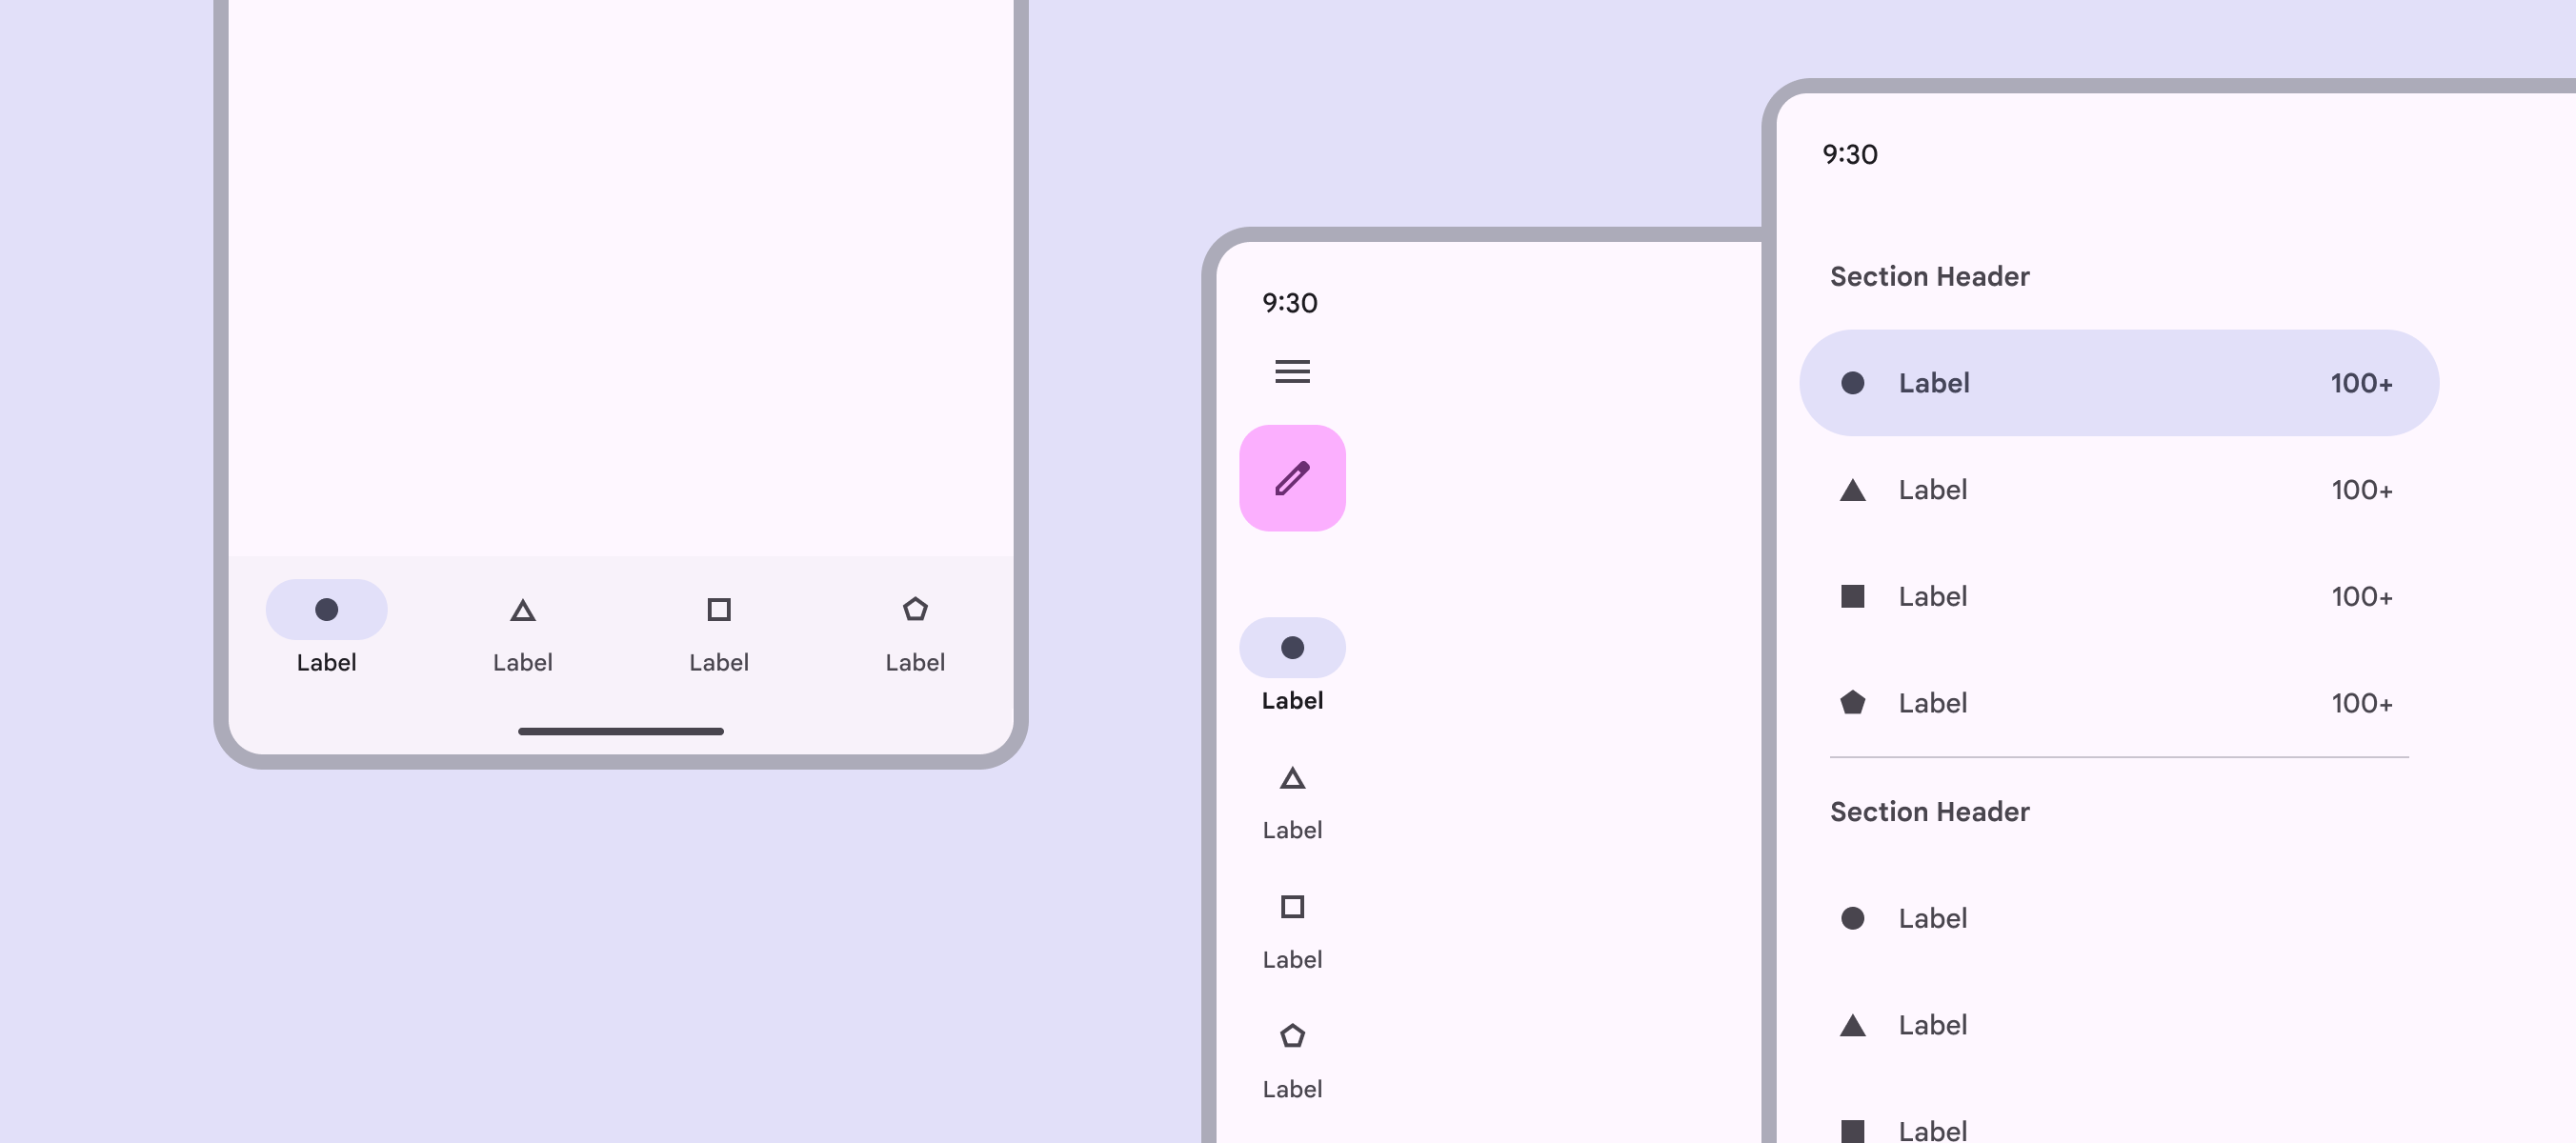
\includegraphics[width=\textwidth]{images/navigation1.png}
  \caption{Navigační prvky -- převzato z~\cite{layout-m3}}
  \label{fig:navigation}
\end{figure}

\begin{figure}
  \centering 
  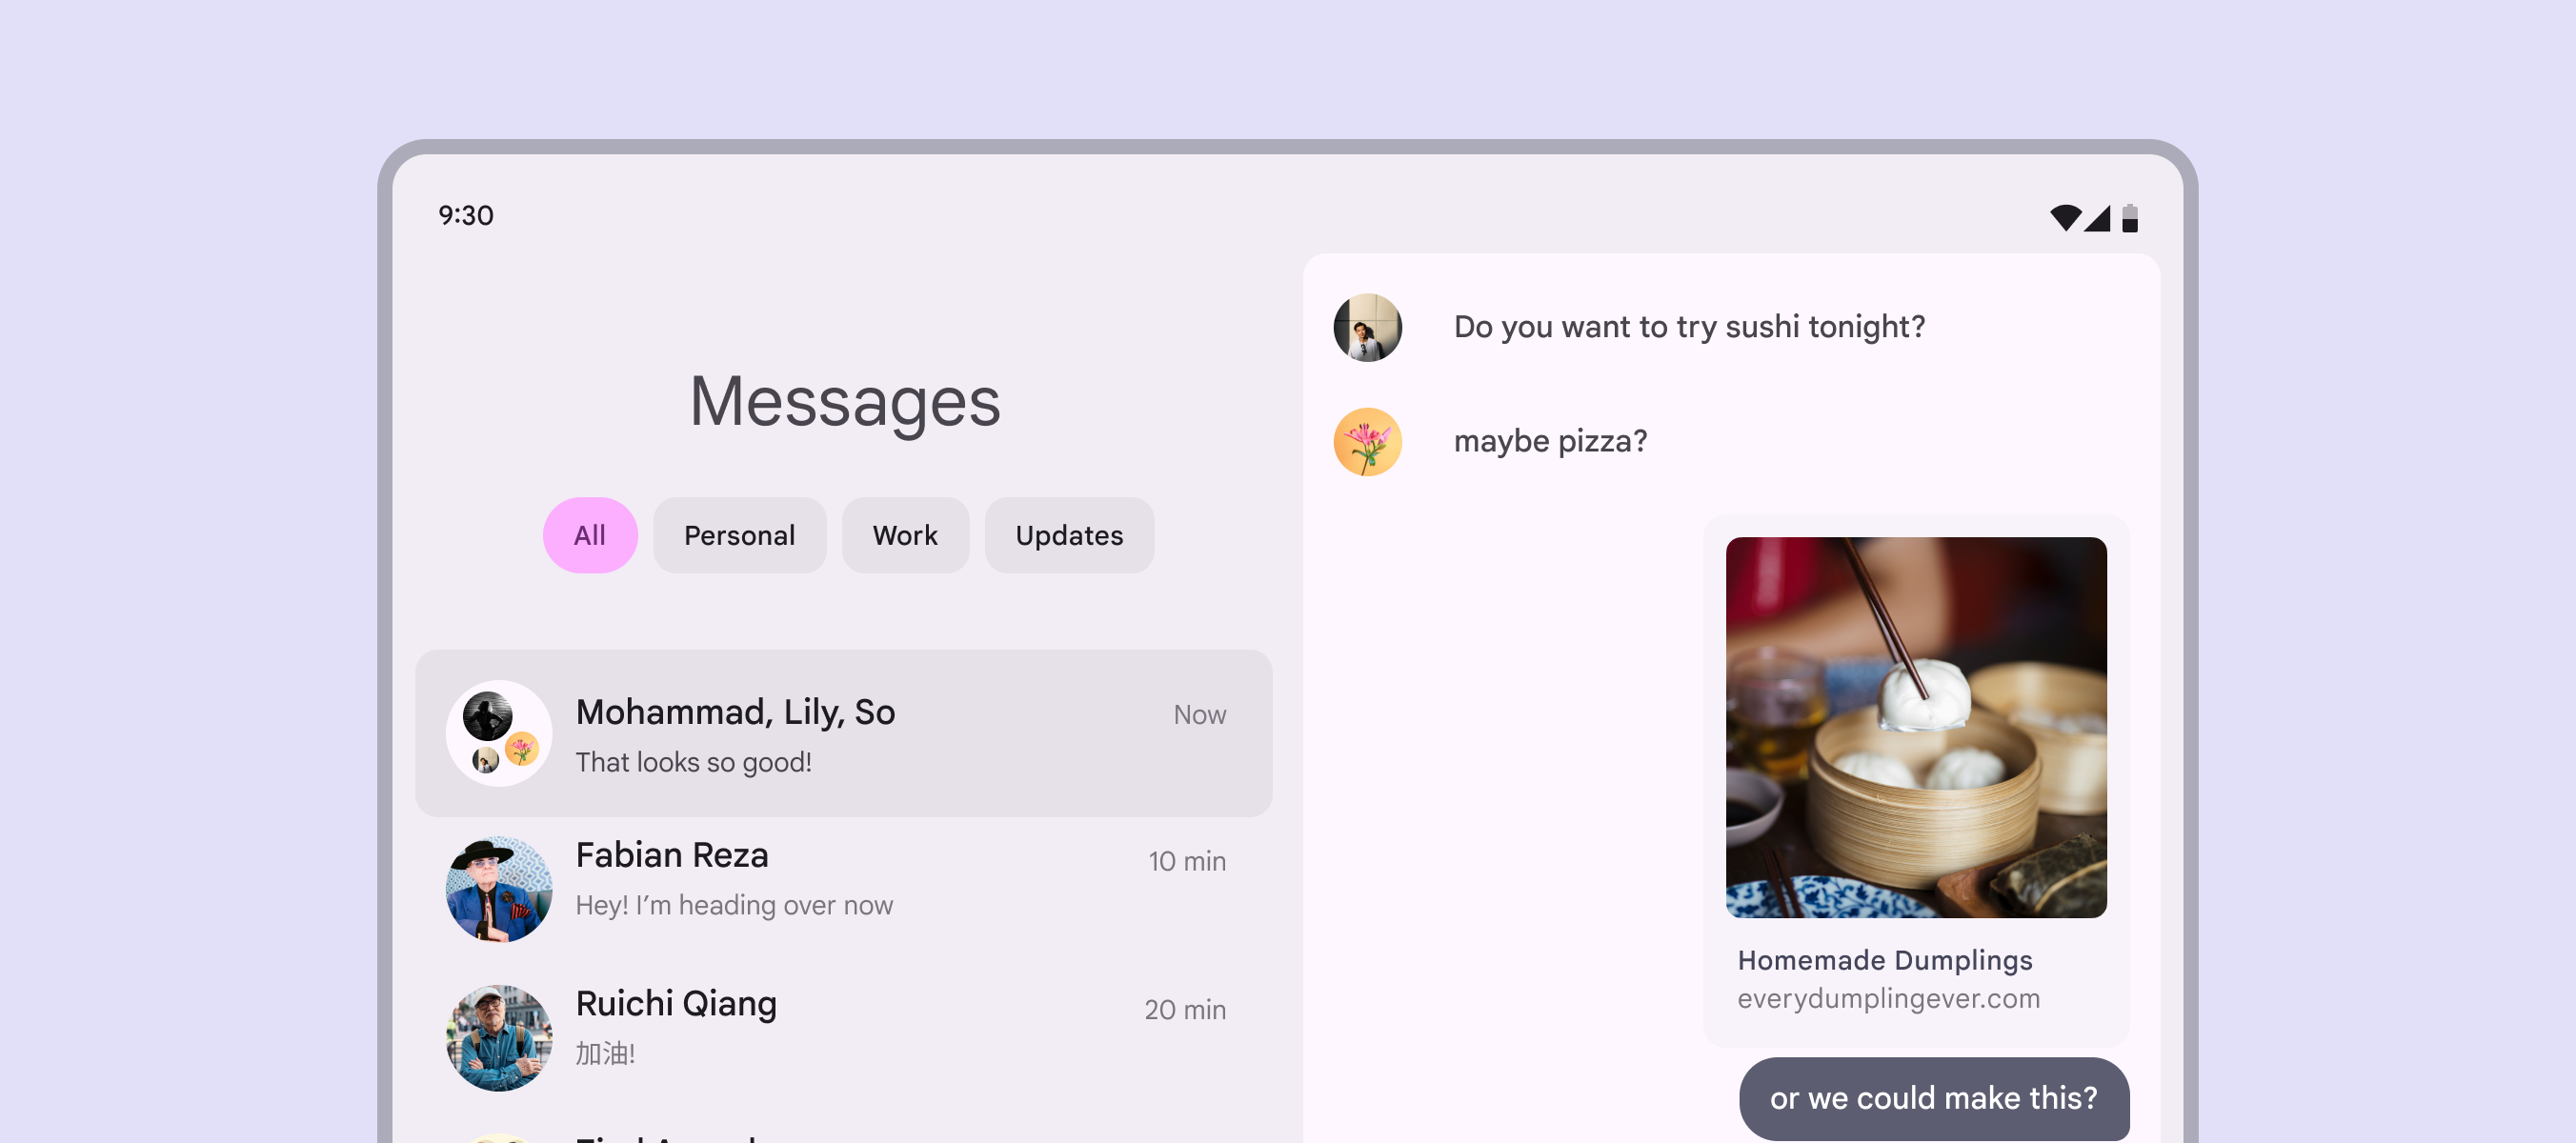
\includegraphics[width=\textwidth]{images/canonical-layout.png}
  \caption{Kanonické rozložení -- převzato z~\cite{m3}}
  \label{fig:canonical-layout}
\end{figure}

\subsection{Vizuální část aplikace}
Vizuální část aplikace je z~pohledu uživatele velmi důležitá. Řadí se do ní barvy v~aplikaci, ikona aplikace, použité fonty atd. Primární barvou aplikace jsem zvolil tmavě tyrkysovou. Je nastavená jako výchozí barva v~barevném tématu a použil jsem ji i pro ikonu aplikace. Ikona aplikace (viz \hyperref[fig:app-icon]{Obrázek \ref{fig:appicon}}) byla vytvořena v~nástroji Figma. Byly v~ní použity ikony z~Google Fonts. Jako font aplikace jsme zvolil font \textit{Poppins}, který je podobný doporučenému fontu \textit{Roboto} ze systému Material Design. Fonty jsou vidět na obrázku \ref{fig:font}. 

\begin{figure}
  \centering
  
\includegraphics[width=0.35\textwidth]{images/app-icon.pdf}
  \caption{Ikona aplikace}
  \label{fig:appicon}
\end{figure}

\begin{figure}
  \centering
  
\includegraphics[width=\textwidth]{images/font-comparision.pdf}
  \caption{Font Roboto (nahoře) a Poppins (dole)}
  \label{fig:font}
\end{figure}

\subsection{Zajímavosti při tvorbě práce}
Tvorba aplikace oproti návrhu místy přinese neplánované komplikace, které je nutné řešit nebo redefinovat požadavek. I~v~tomto projektu jsem se s~touto výzvou setkal.

\begin{itemize}
  \item \textbf{Problém s~výběrem SQLite balíčku} nastal hned ze začátku programování aplikace. Při postupování podle dokumentace \cite{flutter-docs}, která ukazuje práci s~balíčkem sqflite, jsem při čtení dokumentace balíčku zjistil, že balíček podporuje pouze Android, iOS a macOS. Vzhledem k~zamýšlenému provozu i na jiných platformách bylo nutné najít alternativu. Objeveil jsem balíček Drift, který podporuje všechny platformy. Navíc přinesl i bonus v~podobě kvalitní API pro dotazování nad databází bez použití jazyka SQL.
  \item \textbf{Nekompletní podpora všech komponent Material Design}. Přestože framework Flutter i systém Material Design mají stejného vývojáře firmu Google, není jejich propojení 100\%. Flutter většinu komponent implementuje bez problémů, ale některé nejsou vůbec podporovány, případně je jejich použití omezené. Jako příklad uvedu komponentu \kiinlinecode{}{;}{BottomSheet}, která je vidět na \hyperref[fig:bottomsheet]{obrázku \ref{fig:bottomsheet}} a slouží ke zobrazení doplňkového obsahu a akcí. Případně \kiinlinecode{}{;}{LayoutBuilder} sloužící k~tvorbě responzivního designu. Programátor musí problémy, které běžně řeší tyto komponenty, nahradit nebo jejich řešení implementovat sám.
  \begin{figure}
    \centering
    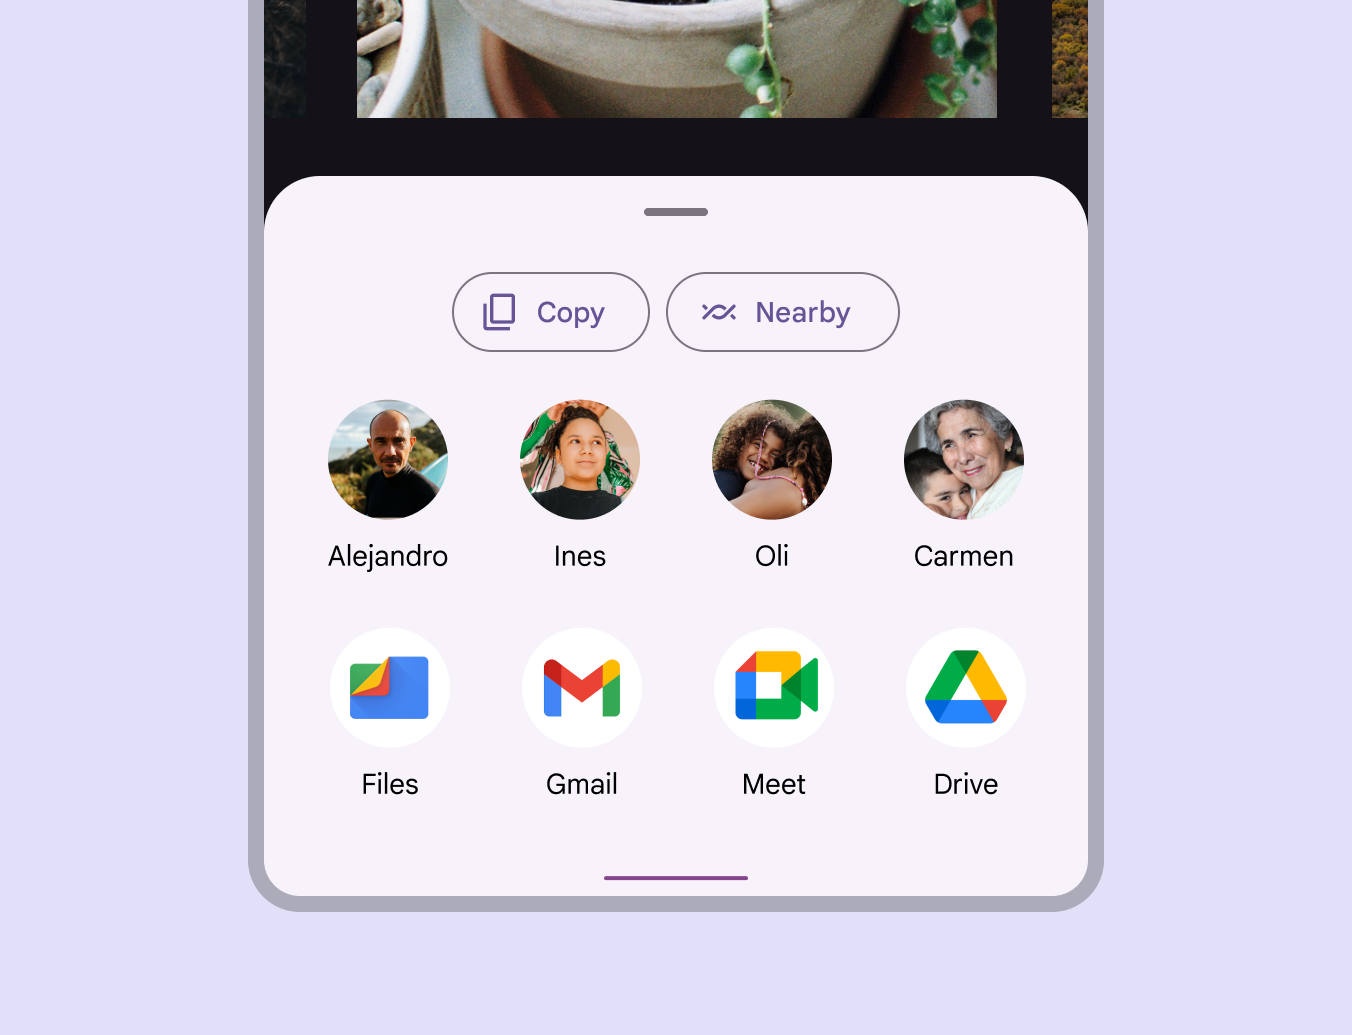
\includegraphics[width=0.7\textwidth]{images/bottom-sheet.png}
    \caption{Komponenta BottomSheet -- převzato z~\cite{m3}}
    \label{fig:bottomsheet}
  \end{figure}
  \item \textbf{Odstranění kategorií či měn} přináší navazující problém, jak naložit s~transakcemi, které mají danou měnu nebo kategorii přiřazenou. Existují dvě možná řešení -- navázané transakce přenést pod jinou kategorii/měnu podle volby uživatele nebo navázané transakce odstranit. Z~hlediska pohodlnosti jsem zvolil možnost druhou, že dané transakce se spolu s~vybranou kategorií/měnou smažou.
\end{itemize}

\section{Uživatelská příručka}
Aplikaci Budget Buddy pro správu financí lze nainstalovat na operační systém Android verze 5.0 a vyšší a Windows 10 a vyšší se zárukou bezproblémové funkčnosti podle návodu. Pro operační systémy macOS a Linux je nutné aplikaci nejdříve sestavit a následně nainstalovat (tento postup je ponechán na zdatném uživateli). Návod se týka jen vybraných platforem z~důvodu testování. 

\subsection{První spuštění}
Při prvním spuštění se zobrazí rovnou úvodní obrazovka \textit{Dashboard}. Není nutné se přihlašovat, aplikace je nyní určena pouze pro jednoho uživatele a běží lokálně. Pro první spuštění jsou předpřipravené základní kategorie transakcí a nejběžnější měny (obojí je možno upravit). 

\subsection{Úvodní obrazovka}
Úvodní obrazovka (viz \hyperref[fig:dashboard-large]{Obrázek \ref{fig:dashboard-large}}) je centrem dění pro uživatele. Poskytuje základní přehled o~finanční situaci. Konkrétně zobrazuje graf útraty podle kategorií (v~aktuálním měsíci), stav účtu, dnešní útratu a posledních pět transakcí. Pro zařízení s~větší obrazovkou je rozšířena o~legendu grafu a další zajímavé číselné údaje o~stavu účtu. Úvodní obrazovka není uživatelsky přizpůsobitelná.

\begin{figure}
  \centering
  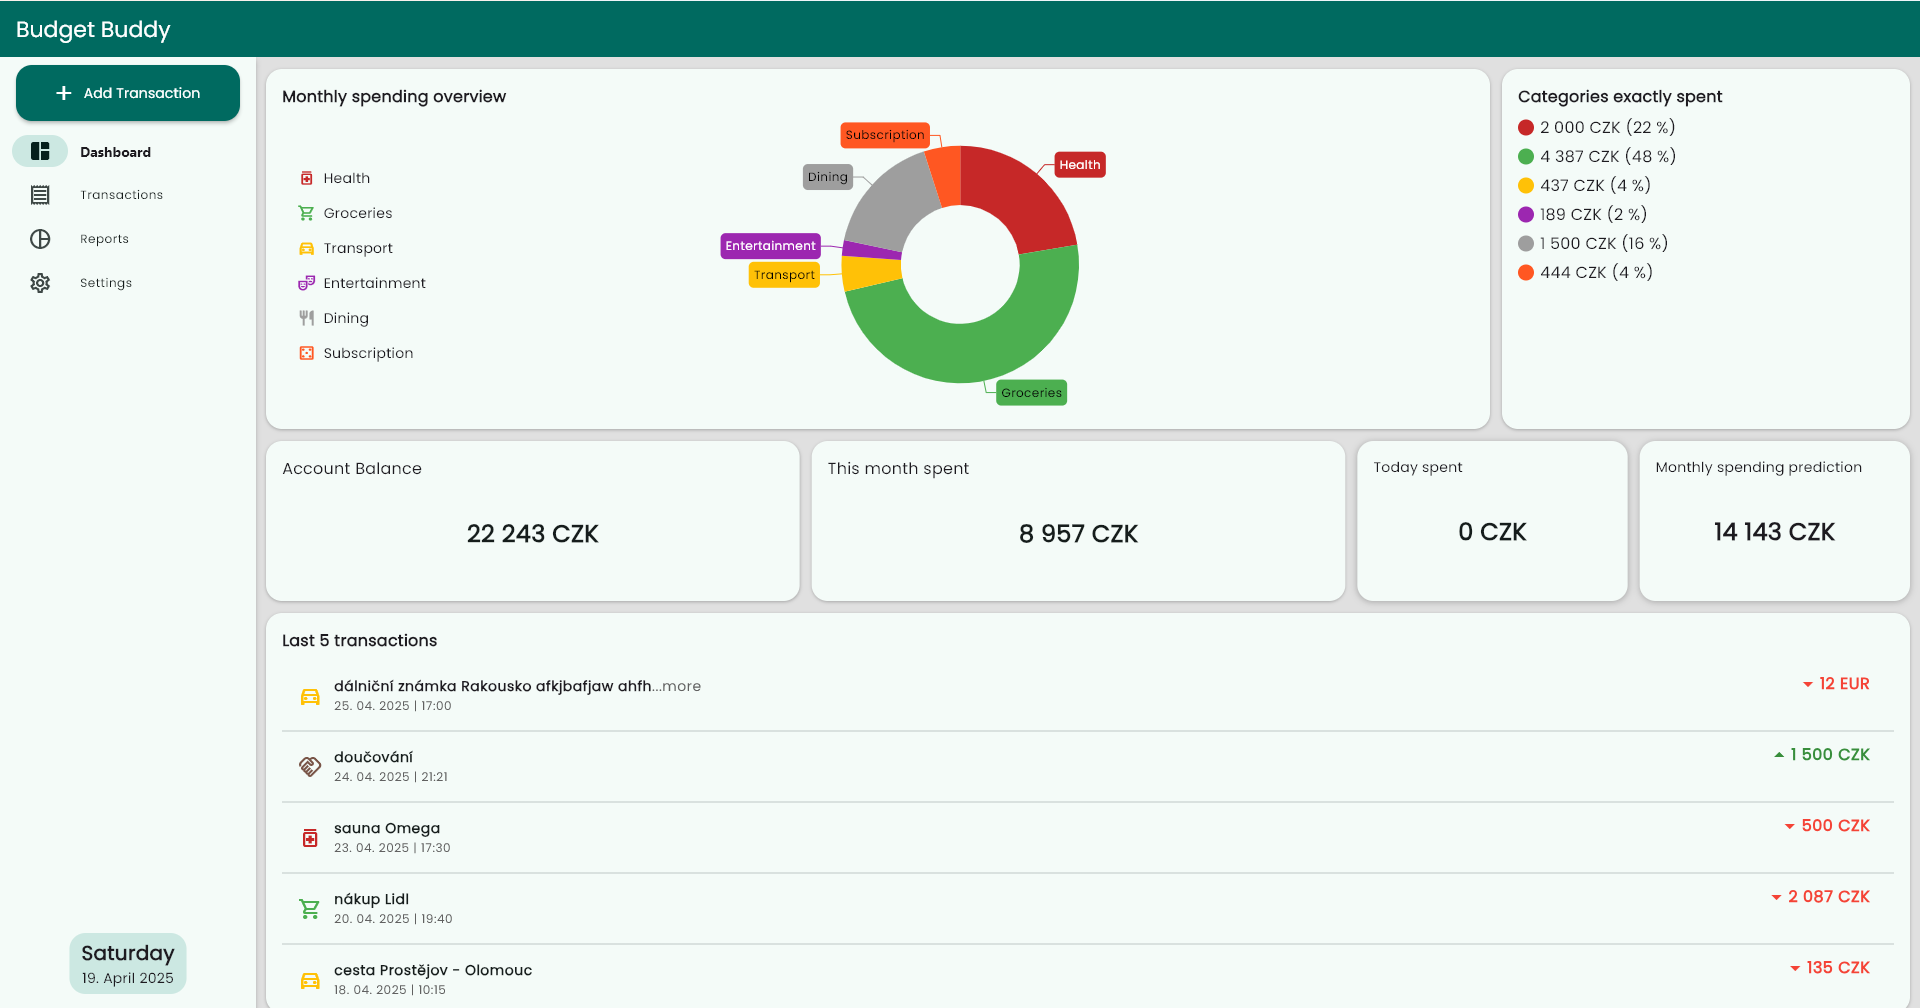
\includegraphics[width=\textwidth]{images/dashboard-large.png}
  \caption{Obrazovka \textit{Dashboard} na desktopovém zařízení}
  \label{fig:dashboard-large}
\end{figure}

\subsection{Přidání transakce}
Transakce se přidává tlačítkem označeným ikonou plus, na větším zařízení i doplňujícím popiskem. Na menším zařízení se tlačítko nachází v~pravé dolní části obrazovky nad navigační lištou jako tzv. \textit{floating action button}. Na větším zařízení je umístěno před prvním prvkem v~navigační liště na pravé straně obrazovky. Po stisknutí se objeví dialogové okno, které je vidět na \hyperref[fig:add-transaction]{obrázku \ref{fig:add-transaction}}, kde uživatel může vybrat z~následujících možností:
\begin{itemize}
  \item \textbf{Částka} -- zadává se hodnota transakce jako číslo. Desetinná čísla jsou povolená jak s~čárkou i s~tečkou (čárku si aplikace sama převede na tečku).
  \item \textbf{Poznámka} -- textový doplněk transakce o~délce maximálně 1000 znaků.  Poznámka není povinná.
  \item \textbf{Typ} -- výběr ze dvou možností zda-li jde o~útratu nebo příjem.
  \item \textbf{Kategorie} -- kategorie se kterou bude transakce spojena. Výběr se zobrazí ve vyjíždějícím seznamu po kliknutí.
  \item \textbf{Měna} -- měna dané transakce. Pokud se jedná o~měnu jinou než Česká koruna, bude provedena konverze podle aktuálně nastaveného kurzu.
  \item \textbf{Datum} -- jaký den byla transakce provedena. Předvyplněno na aktuální datum.
  \item \textbf{Čas} -- v~jakou denní dobu byla transakce provedena. Předvyplněno na aktuální čas.
\end{itemize}
Vyplněnou transakci je nutné tlačítkem \textit{Save Transaction} uložit jinak nebude zápis proveden.

\begin{figure}
  \centering
  \raisebox{0.2\height}{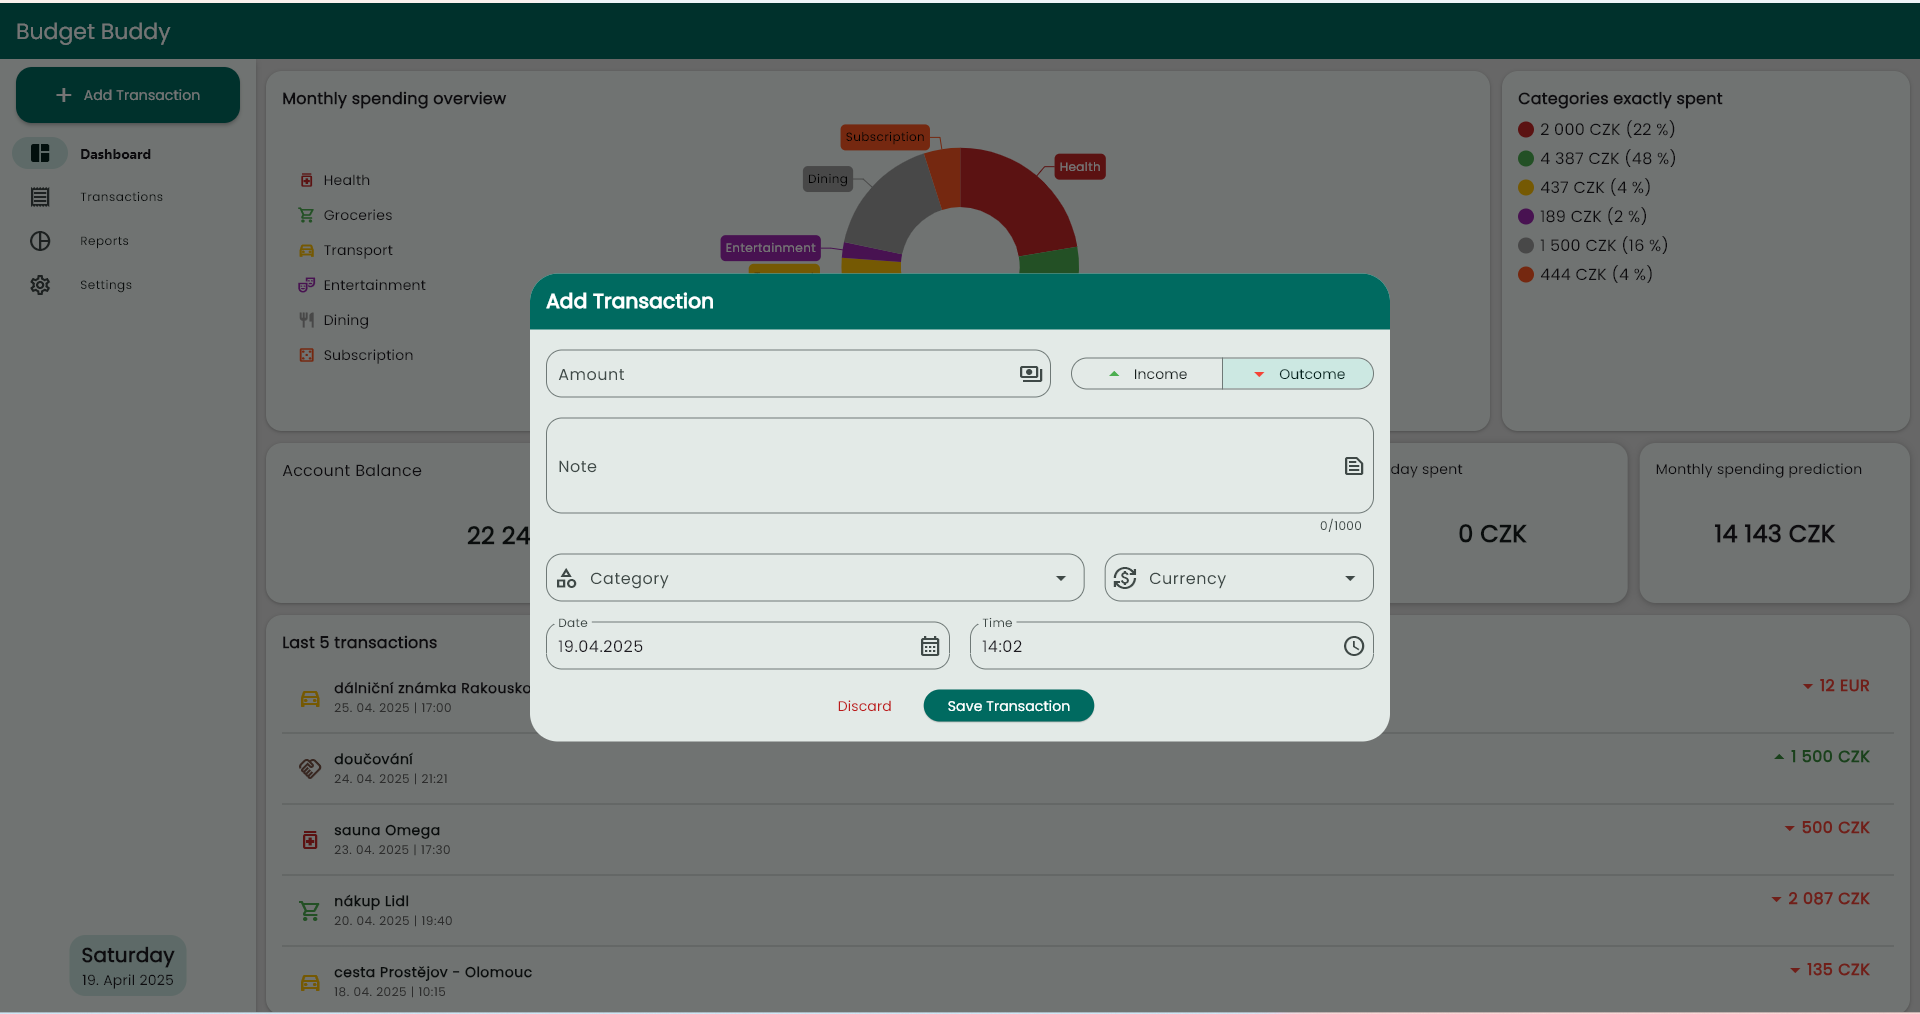
\includegraphics[width=0.69\textwidth]{images/add-transaction-large.png}}%
  \hspace{0.5em}%
  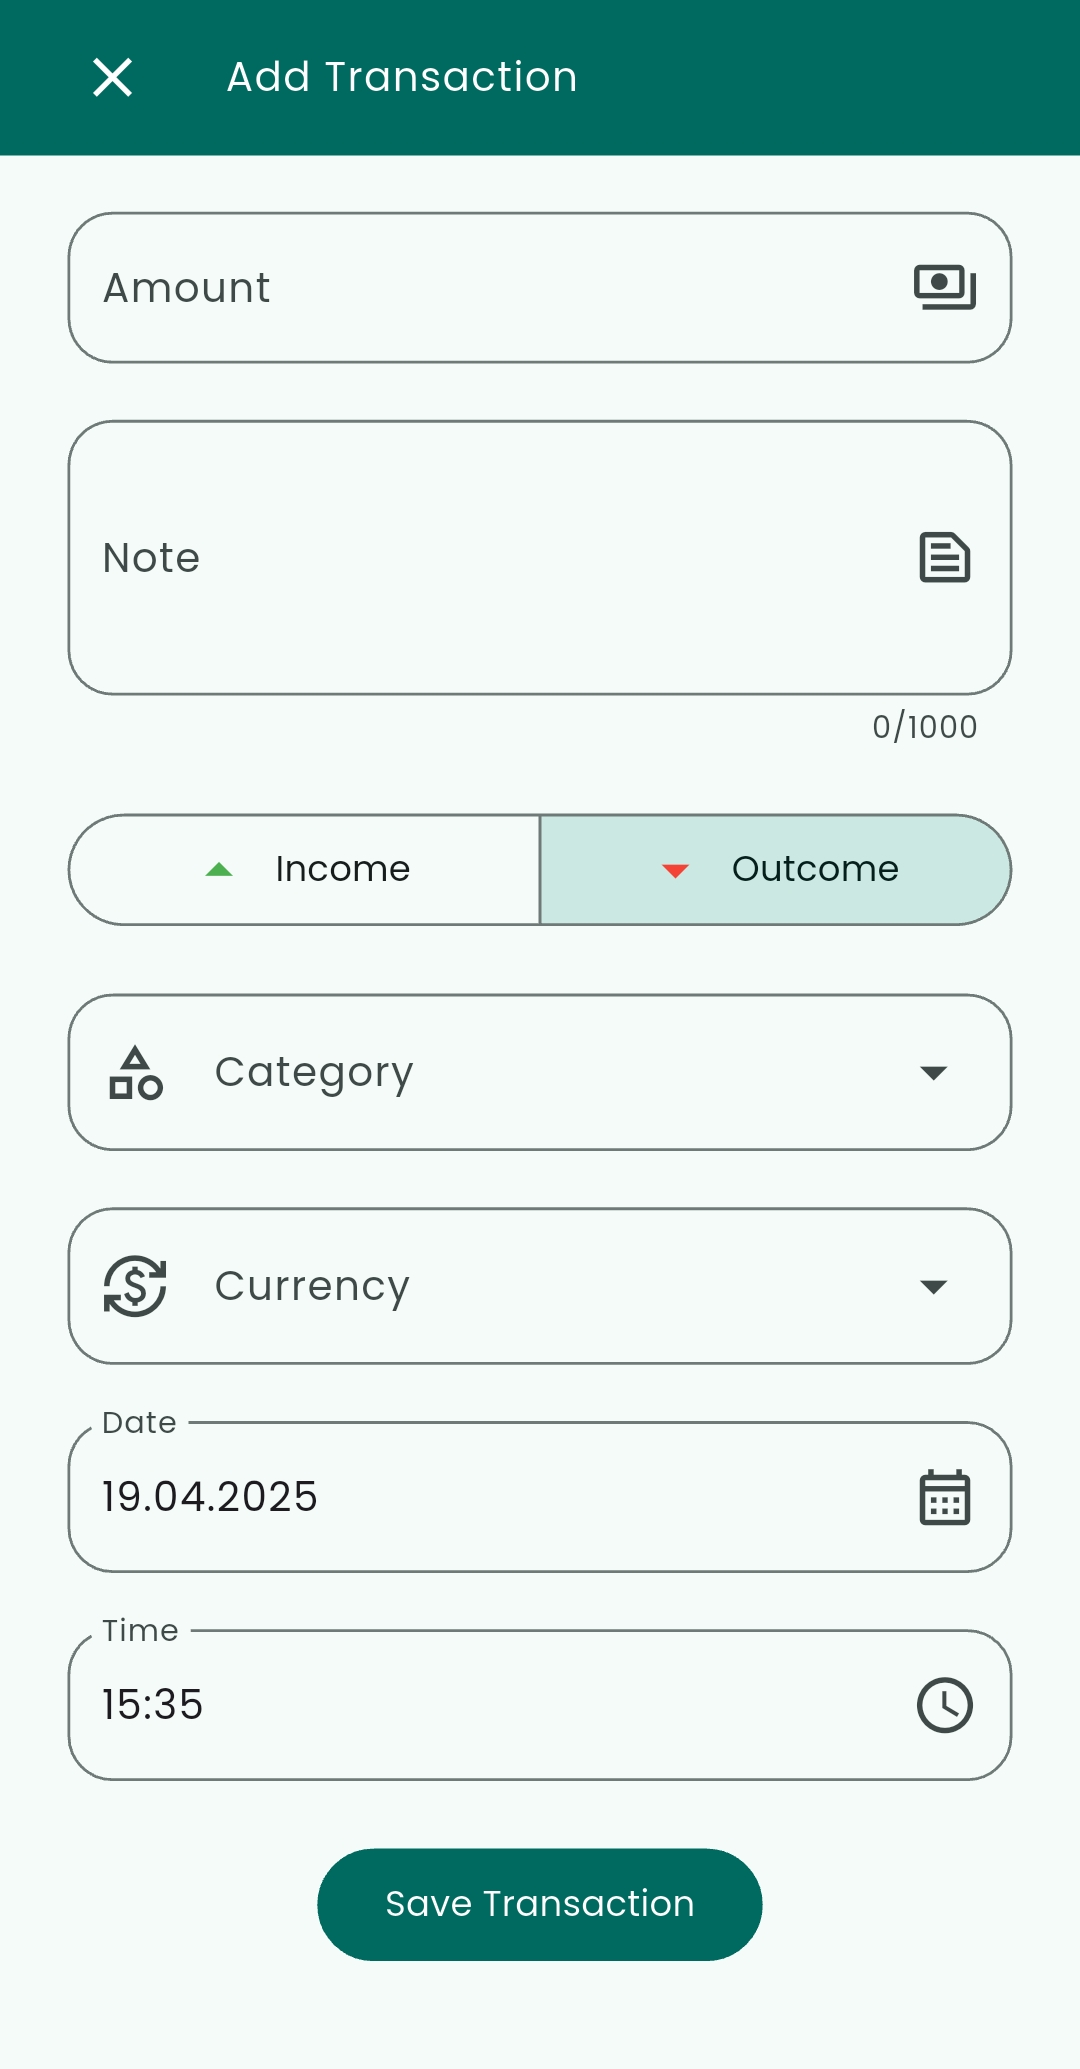
\includegraphics[width=0.28\textwidth]{images/add-transaction-mobile.png}%
  \caption{Dialogové okno pro přidání transakce na desktopovém zařízení (vlevo) a mobilním telefonu (vpravo)}
  \label{fig:add-transaction}
\end{figure}

\subsection{Zobrazení a úprava transakcí}
Výpis transakcí a jejich úprava se provádí na druhé obrazovce s~názvem \textit{Transactions}. Výpis je proveden v~seznamu, kde je přímo vidět kategorie, měna, částka, typ, datum a případná poznámka (viz \hyperref[fig:dashboard-transactions-mobile]{Obrázek \ref{fig:dashboard-transactions-mobile}}). Po kliknutí na transakci se objeví dialogové okno a je možné všechny parametry transakce upravit (viz \hyperref[fig:transactions-edit]{Obrázek \ref{fig:transactions-edit}} vlevo), případně transakci odstranit. Transakce je možné filtrovat dvěma způsoby (viz \hyperref[fig:transactions-edit]{Obrázek \ref{fig:transactions-edit}} vpravo). Můžeme nechat zobrazit jen transakce ve specifickém období (den, týden, měsíc, rok či libovolný rozsah), k~čemuž slouží prostřední tlačítko v~horní části zobrazující aktuálně zvolené období. Šipky na stranách umožňují přesouvat se o~zvolené období dozadu či dopředu. Dále můžeme vybírat ze všech parametrů, které jsou transakci přiřazené (kategorie, měna, typ atd.). Obrazovka s~výběrem filtrů se otevře při stisknutí tlačítka \textit{Filter} s~ikonou trychtýře. Při použití více filtrů se transakce zobrazí ve výpisu pokud splňuje alespoň jednu podmínku. Aktivní filtry znázorňuje červený odznak u~tlačítka filtrace.

\begin{figure}
  \centering
  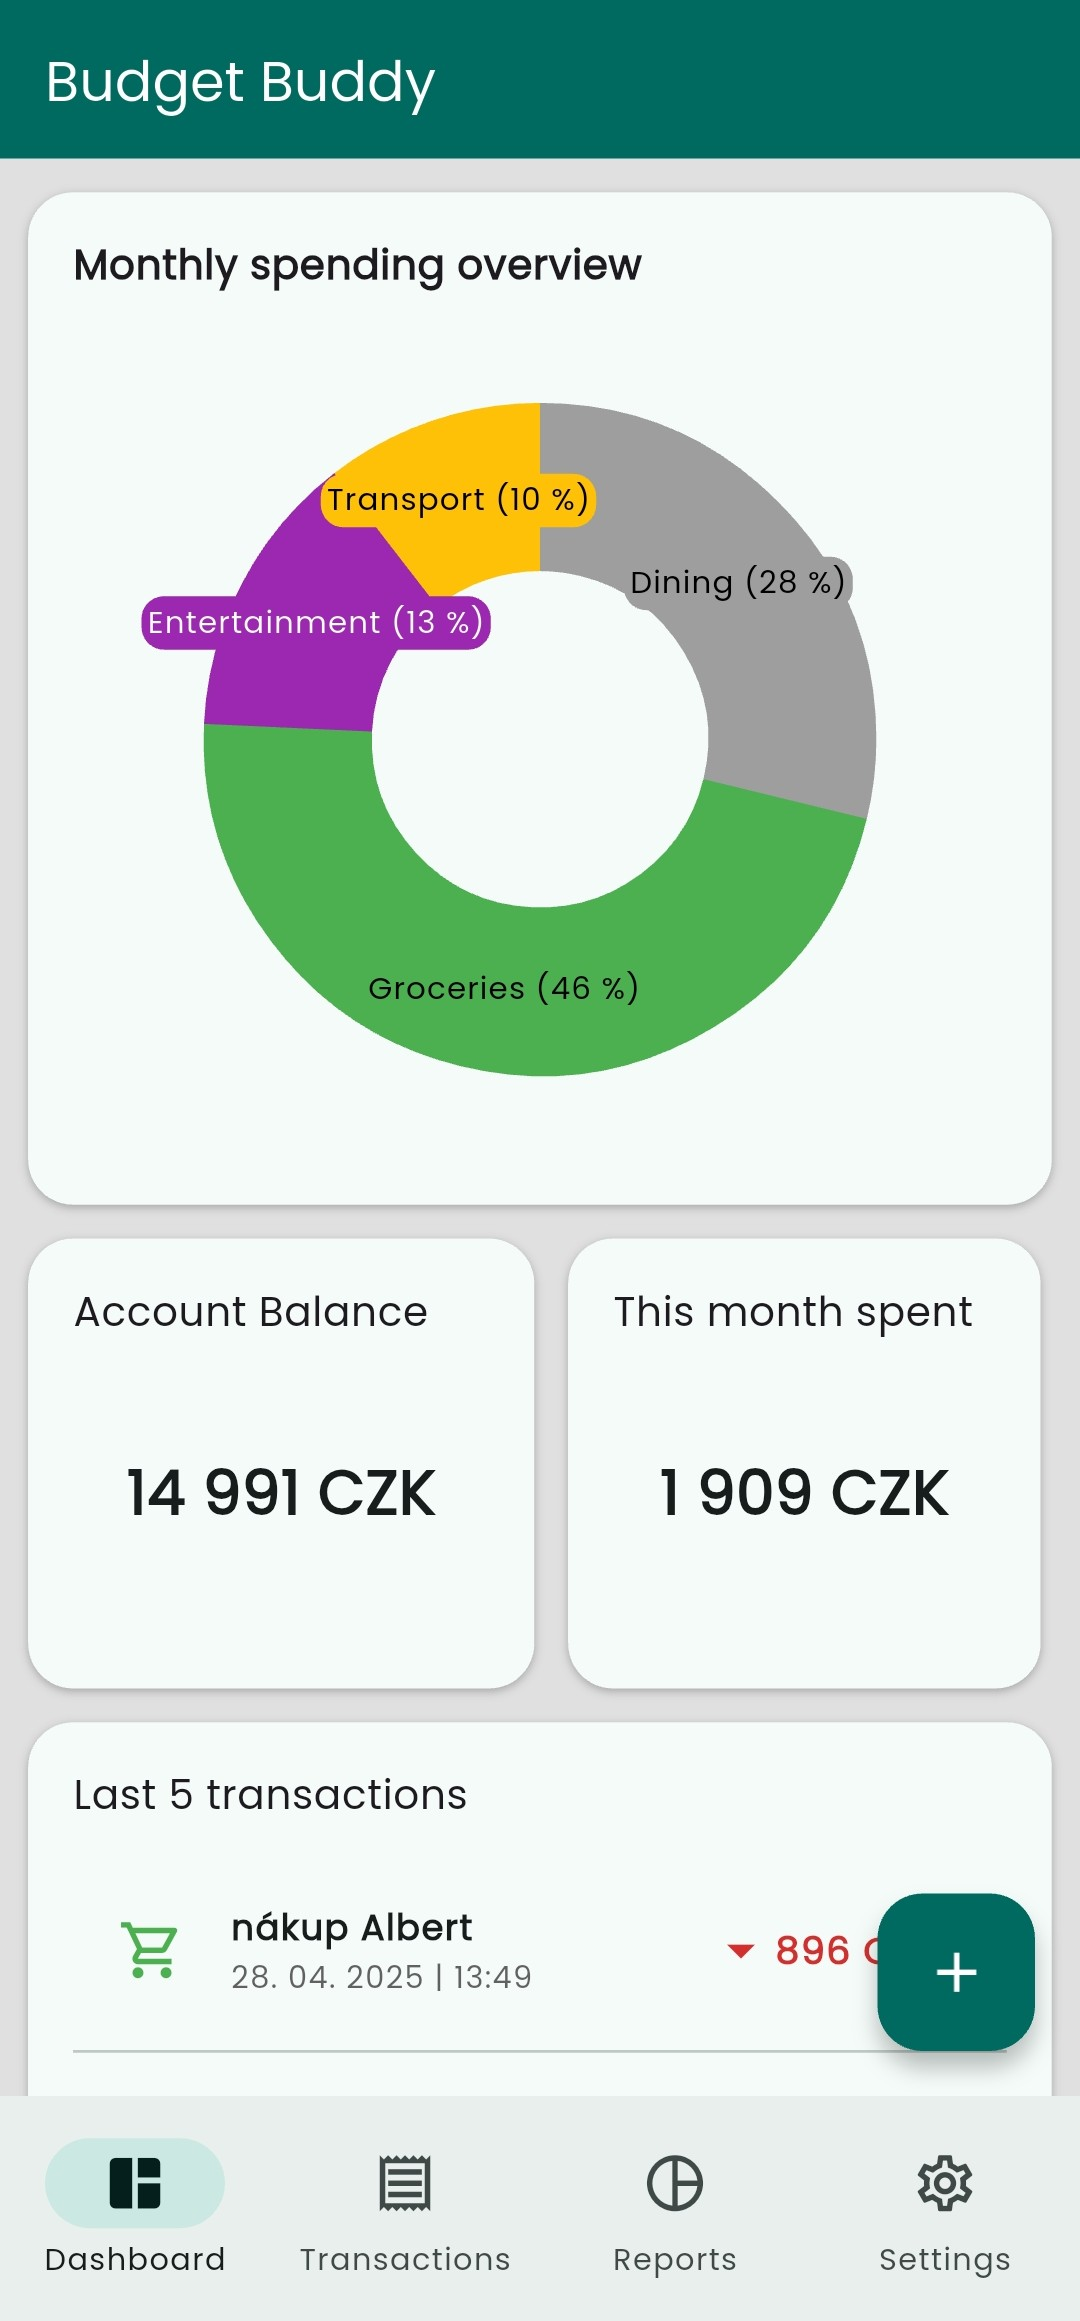
\includegraphics[width=0.45\textwidth]{images/dashboard-mobile.png}
  \hspace{0.5em}
  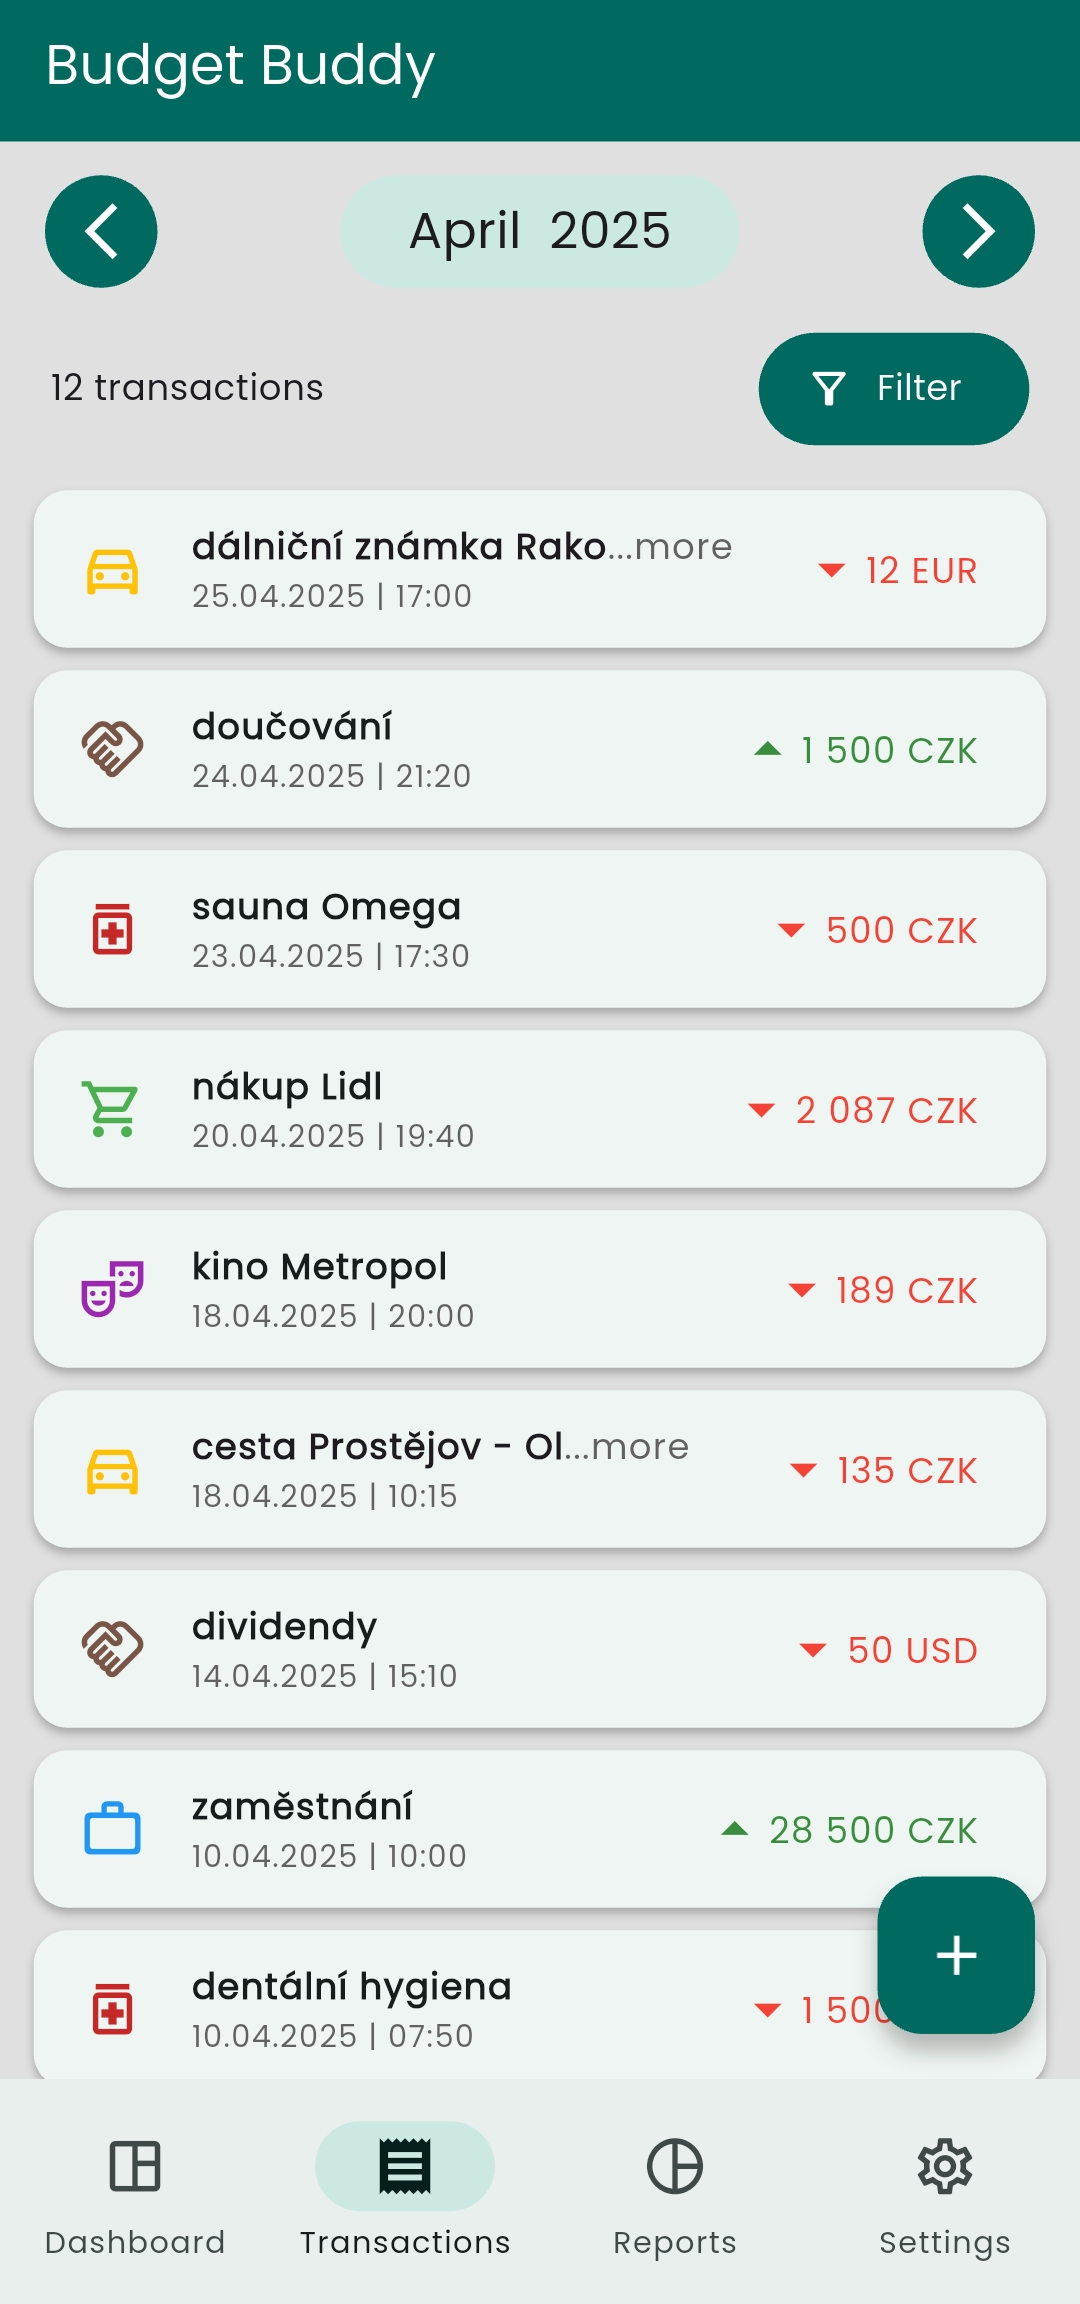
\includegraphics[width=0.45\textwidth]{images/transactions-mobile.png}
  \caption{Obrazovky \textit{Dashboard} a \textit{Transactions} na mobilním telefonu}
  \label{fig:dashboard-transactions-mobile}
\end{figure}

\begin{figure}
  \centering
  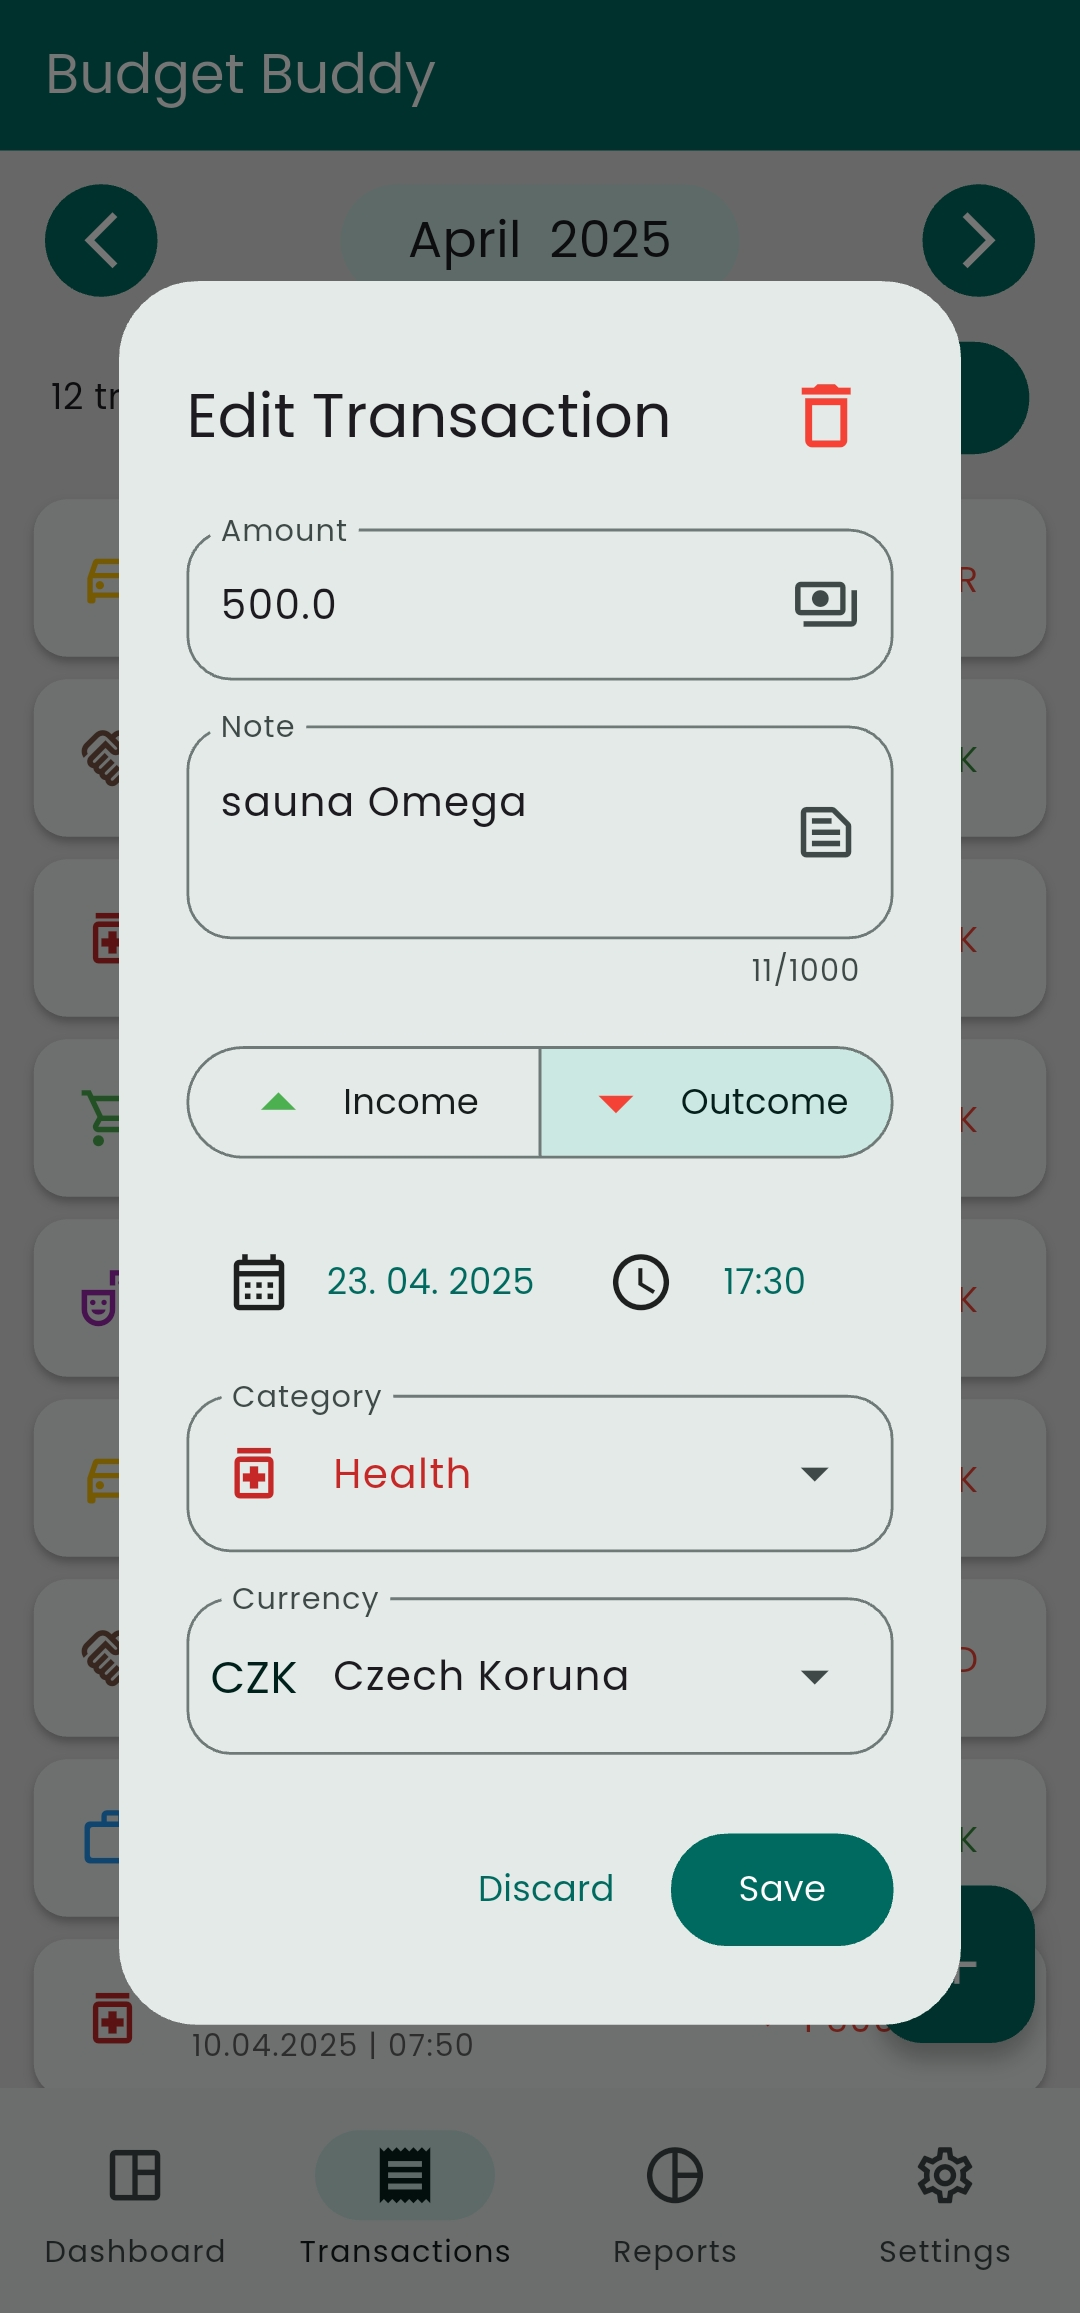
\includegraphics[width=0.45\textwidth]{images/edit-transaction-mobile.png}
  \hspace{0.5em}
  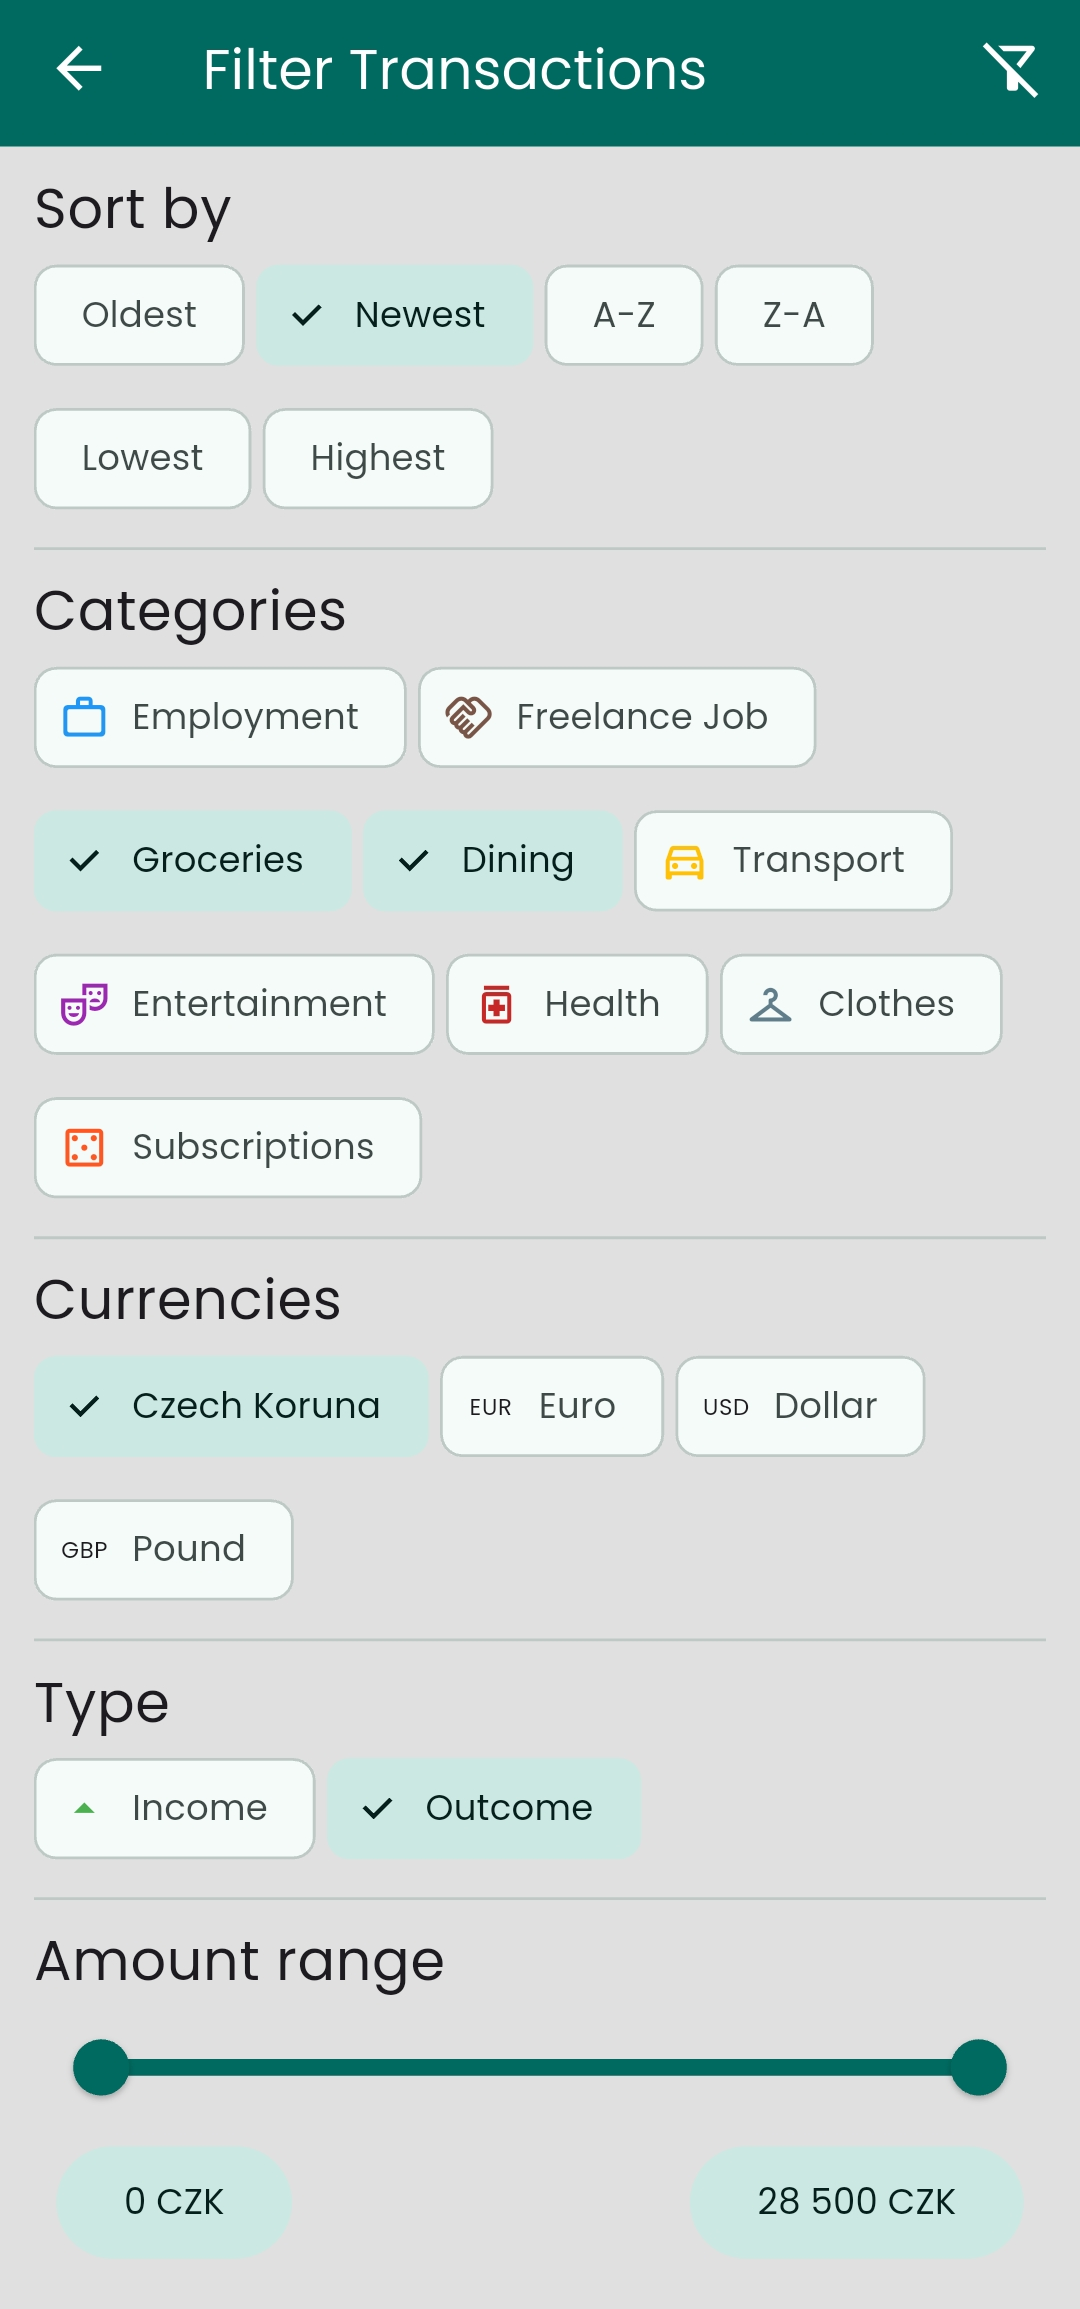
\includegraphics[width=0.45\textwidth]{images/filters-mobile.png}
  \caption{Úprava a filtrace transakcí na mobilním zařízení}
  \label{fig:transactions-edit}
\end{figure}

\subsection{Využití reportů}
Grafy a důležité číselné údaje se nachází na obrazovce \textit{Reports} (viz \hyperref[fig:reports]{Obrázek \ref{fig:reports}}). Je zde na výběr z~pěti přednastavených možností. Které údaje chce uživatel vidět se dá nastavit tlačítkem \textit{Manage reports} pod posledním reportem. Na výběr je z pěti možností:
\begin{itemize}
  \item \textbf{Most spent categories} -- zobrazí sloupcový graf s~pěti kategoriemi, ve~kterých je největší útrata ve~zvoleném období.
  \item \textbf{Spent during time} -- zobrazí plošný graf s~vývojem útraty v~průběhu daného období. Graf je interaktivní a při najetí pohybu kurzorem v~grafu se zobrazí hodnota pro konkrétní datum.
  \item \textbf{Interesting numbers} -- zobrazí tři buňky se zajímavými hodnotami ze zvoleného období. Konkrétně se jedná o: procento ušetřených peněz z~přijmu, průměrnou denní útratu a procento transakcí v~jiné měně, než českých korunách. Podle velikosti zařízení jsou buňky řazeny ve sloupci nebo řádku.
  \item \textbf{Category ratio} -- zobrazí dvě buňky s~kruhovými grafy. První zobrazuje poměr kategorií v~příjmech a druhý poměr kategorií ve~výdajích. Při použití na největším zařízení se zobrazí interaktivní legenda.
  \item \textbf{Income / Outcome numbers} -- zobrazí tři buňky s~číselnými údaji. Konkrétně se jedná o: součet všech příjmů, součet všech výdajů a celkový stav účtu. Podle velikosti zařízení jsou buňky řazeny ve sloupci nebo řádku.
\end{itemize}

\begin{figure}
  \centering
  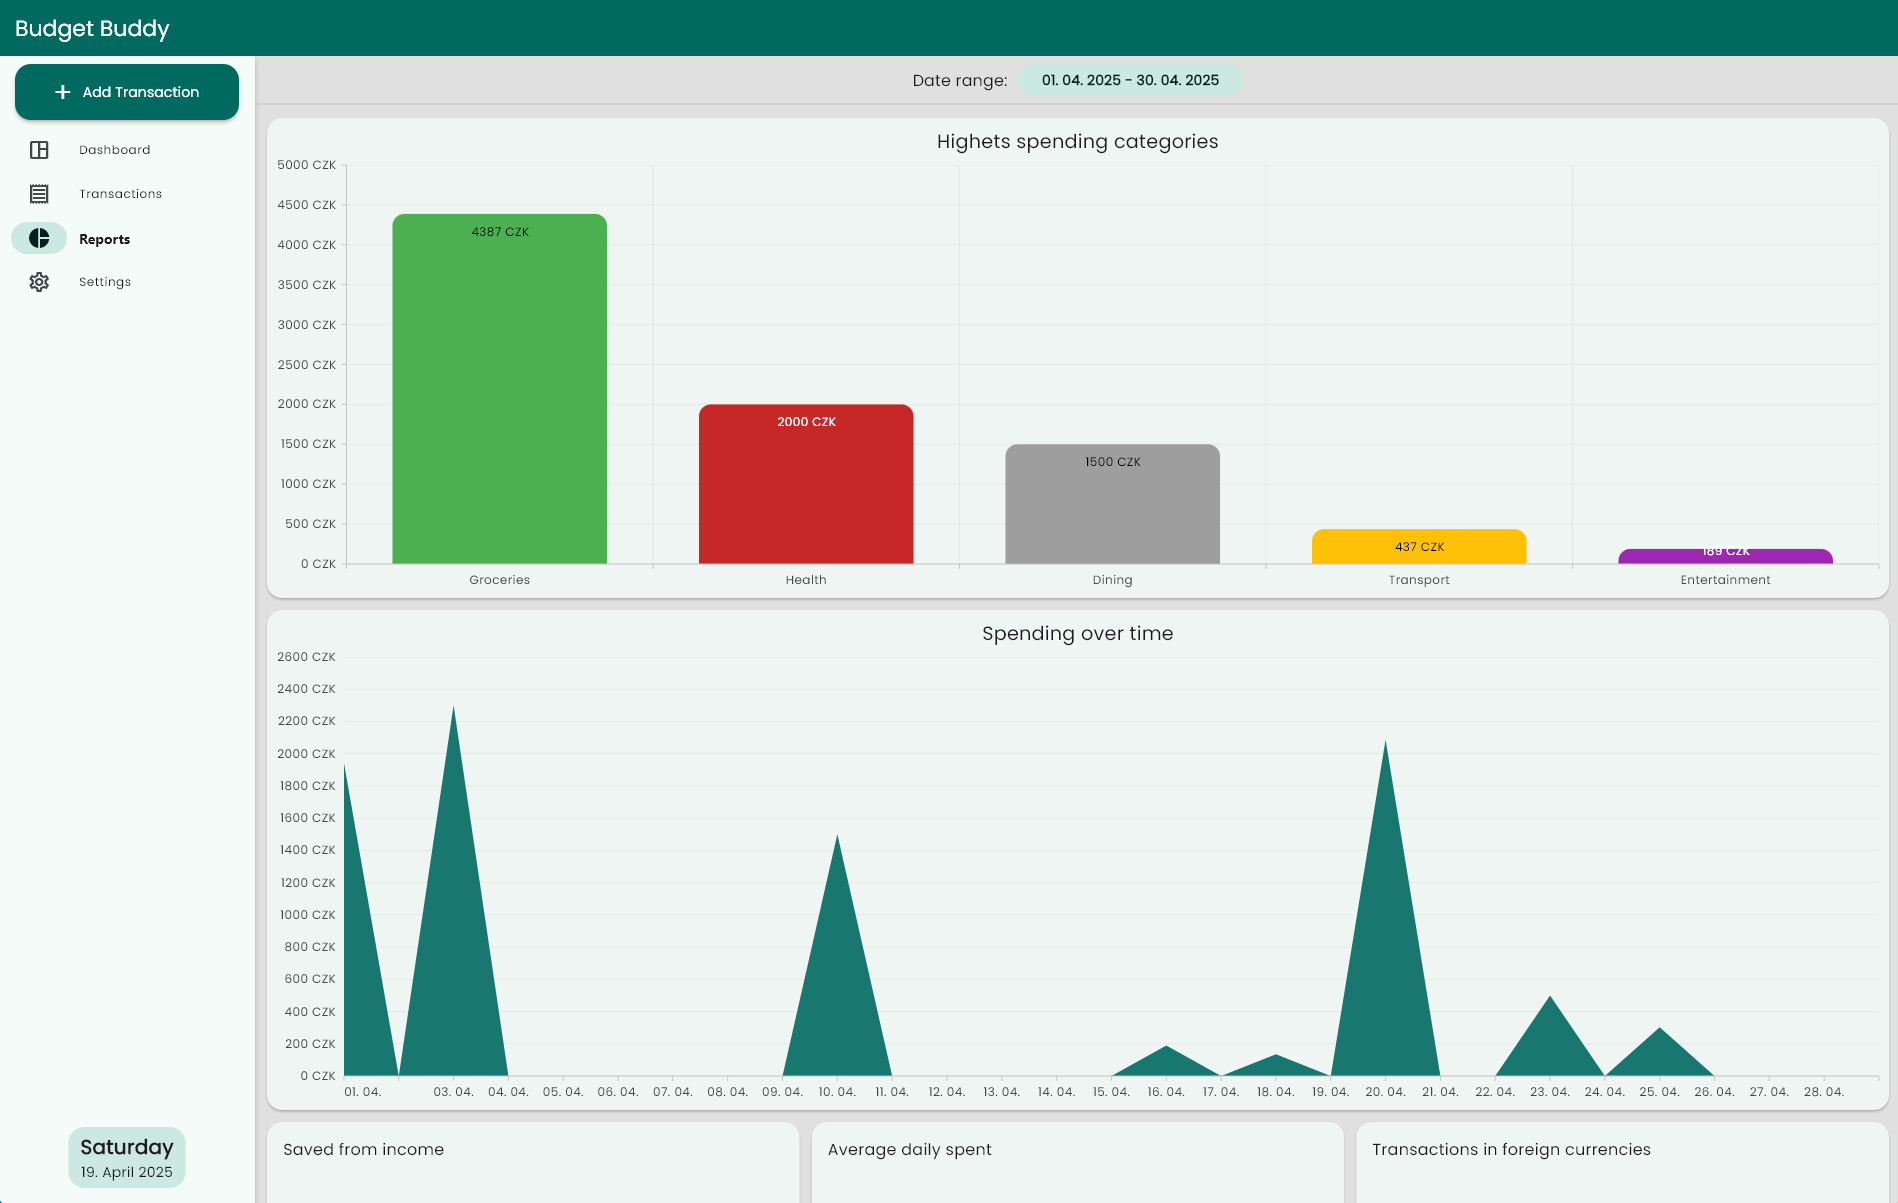
\includegraphics[width=\textwidth]{images/reports-large.png}
  \caption{Obrazovka \textit{Reports} na desktopovém zařízení}
  \label{fig:reports}
\end{figure}

\subsection{Nastavení aplikace}
Poslední obrazovkou dostupnou z~navigační lišty je nastavení (viz \hyperref[fig:settings]{Obrázek \ref{fig:settings}}). Umožňuje nastavit jak prostředí po stránce funkcí, tak i po stránce vzhledu. Taktéž zde uživatel nalezne informace o~aplikaci a možnost smazání všech dat.

\subsubsection{Úprava kategorií}
Přidávat, mazat i upravovat kategorie je možné v~záložce \textit{Categories editor} (viz \hyperref[fig:categories-editor]{Obrázek \ref{fig:categories-editor}}). Otevře se nová obrazovka s~výpisem všech kategorií formou karet. U~každé karty je znázorněna ikona, název a barva. Ikona tužky otevře dialogové okno s~možností upravit nastavení kategorie (změny je nutné uložit tlačítkem \textit{Save}). Ikona popelnice po potvrzení v~dialogovém okně nevratně smaže danou kategorii i ji náležící transakce. Plovoucím tlačítkem s~ikonou plus se vytváří nová kategorie s~uživatelem definovanými parametry.

\begin{figure}
  \centering
  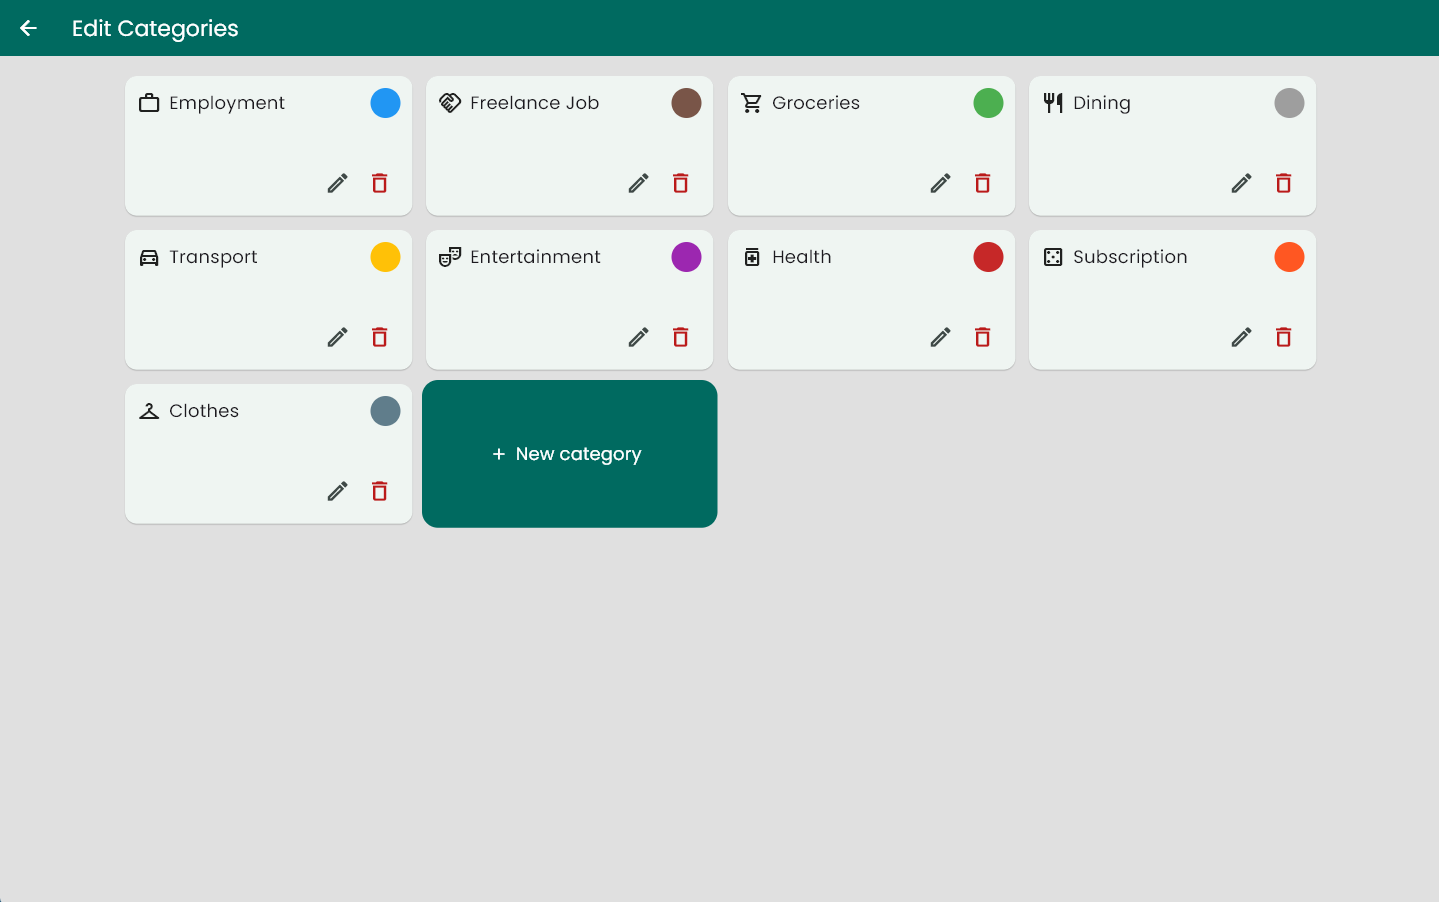
\includegraphics[width=\textwidth]{images/categories-editor-large.png}
  \caption{Obrazovka \textit{Categories editor} na desktopovém zařízení}
  \label{fig:categories-editor}
\end{figure}

\subsubsection{Přizpůsobení měn}
Po kliknutí na kartu \textit{Currency settings} se rozbalí seznam všech měn. V~seznamu je vidět název a zkratka měny. Na pravé straně každé měny je tlačítko \textit{Edit}, které vyvolá dialogové okno pro editaci měny. V~něm je možné zvolit název, směnný kurz a zkratku. Doporučený formát pro zkratku je  ISO~4217 \cite{iso4217}, jelikož zaručuje kompatibilitu s~aktualizací kurzu z~České~národní ~banky. Příklady formátu jsou USD pro dolar, CZK pro Českou korunu nebo EUR pro euro. Aktualizace směnného kurzu se provádí tlačítkem i ikonou šipek v~kruhu. Směnné kurzy jsou čerpány ze stránek České~národní~banky \cite{cnb-kurzy}. Změna kurzu nemá vliv na v~minulosti uložené transakce.

\subsubsection{Přizpůsobení vzhledu}
Vzhled je možno přizpůsobit rozbalením karty \textit{Color theme}. Výběr je ze sedmi barev, které jsou pojmenované i s~náhledem konkrétní barvy. Konkrétní barvy reprezentují jednotlivá barevná témata (jedna barva je základem tématu a z~ní se odvíjí barvy ostatní). Výběr tohoto tématu změní celý nádech aplikace od výrazných barev až po jemné barvy v~pozadí. Změna proběhne ihned a není nutné ji potvrzovat.

\begin{figure}
  \centering
  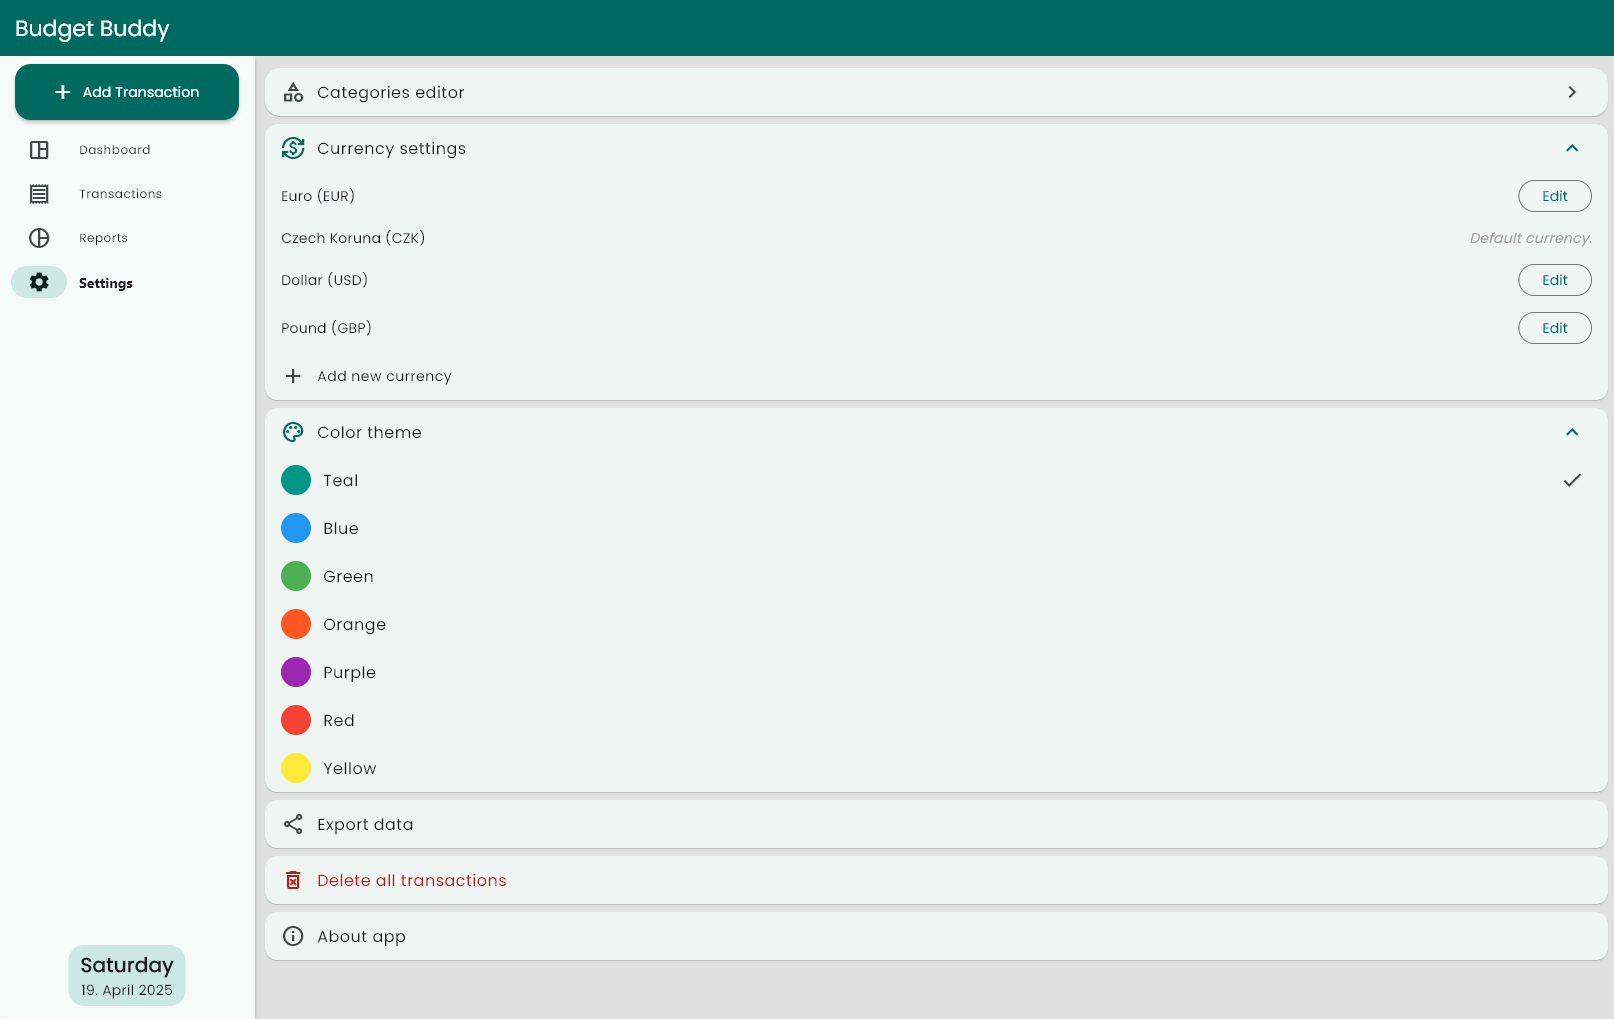
\includegraphics[width=\textwidth]{images/settings-large.png}
  \caption{Obrazovka \textit{Settings} na desktopovém zařízení}
  \label{fig:settings}
\end{figure}

\subsection{Export dat}
Export dat se nachází pod položkou \textit{Export data} (viz \hyperref[fig:export]{Obrázek \ref{fig:export}}). Je možný ve třech formátech -- CSV, JSON a SQLite. První dva formáty slouží především pro import dat do jiných aplikací nebo pro libovolné zpracování uživatelem. Jsou široce podporované a data se dají interpretovat i bez dalšího zpracování. Poslední formát slouží pro zálohu dat. Jde o~soubor s~kompletní SQLite databází. Pro export dat je možné si vybrat libovolné umístění na právě používaném zařízení.

\begin{figure}
  \centering
  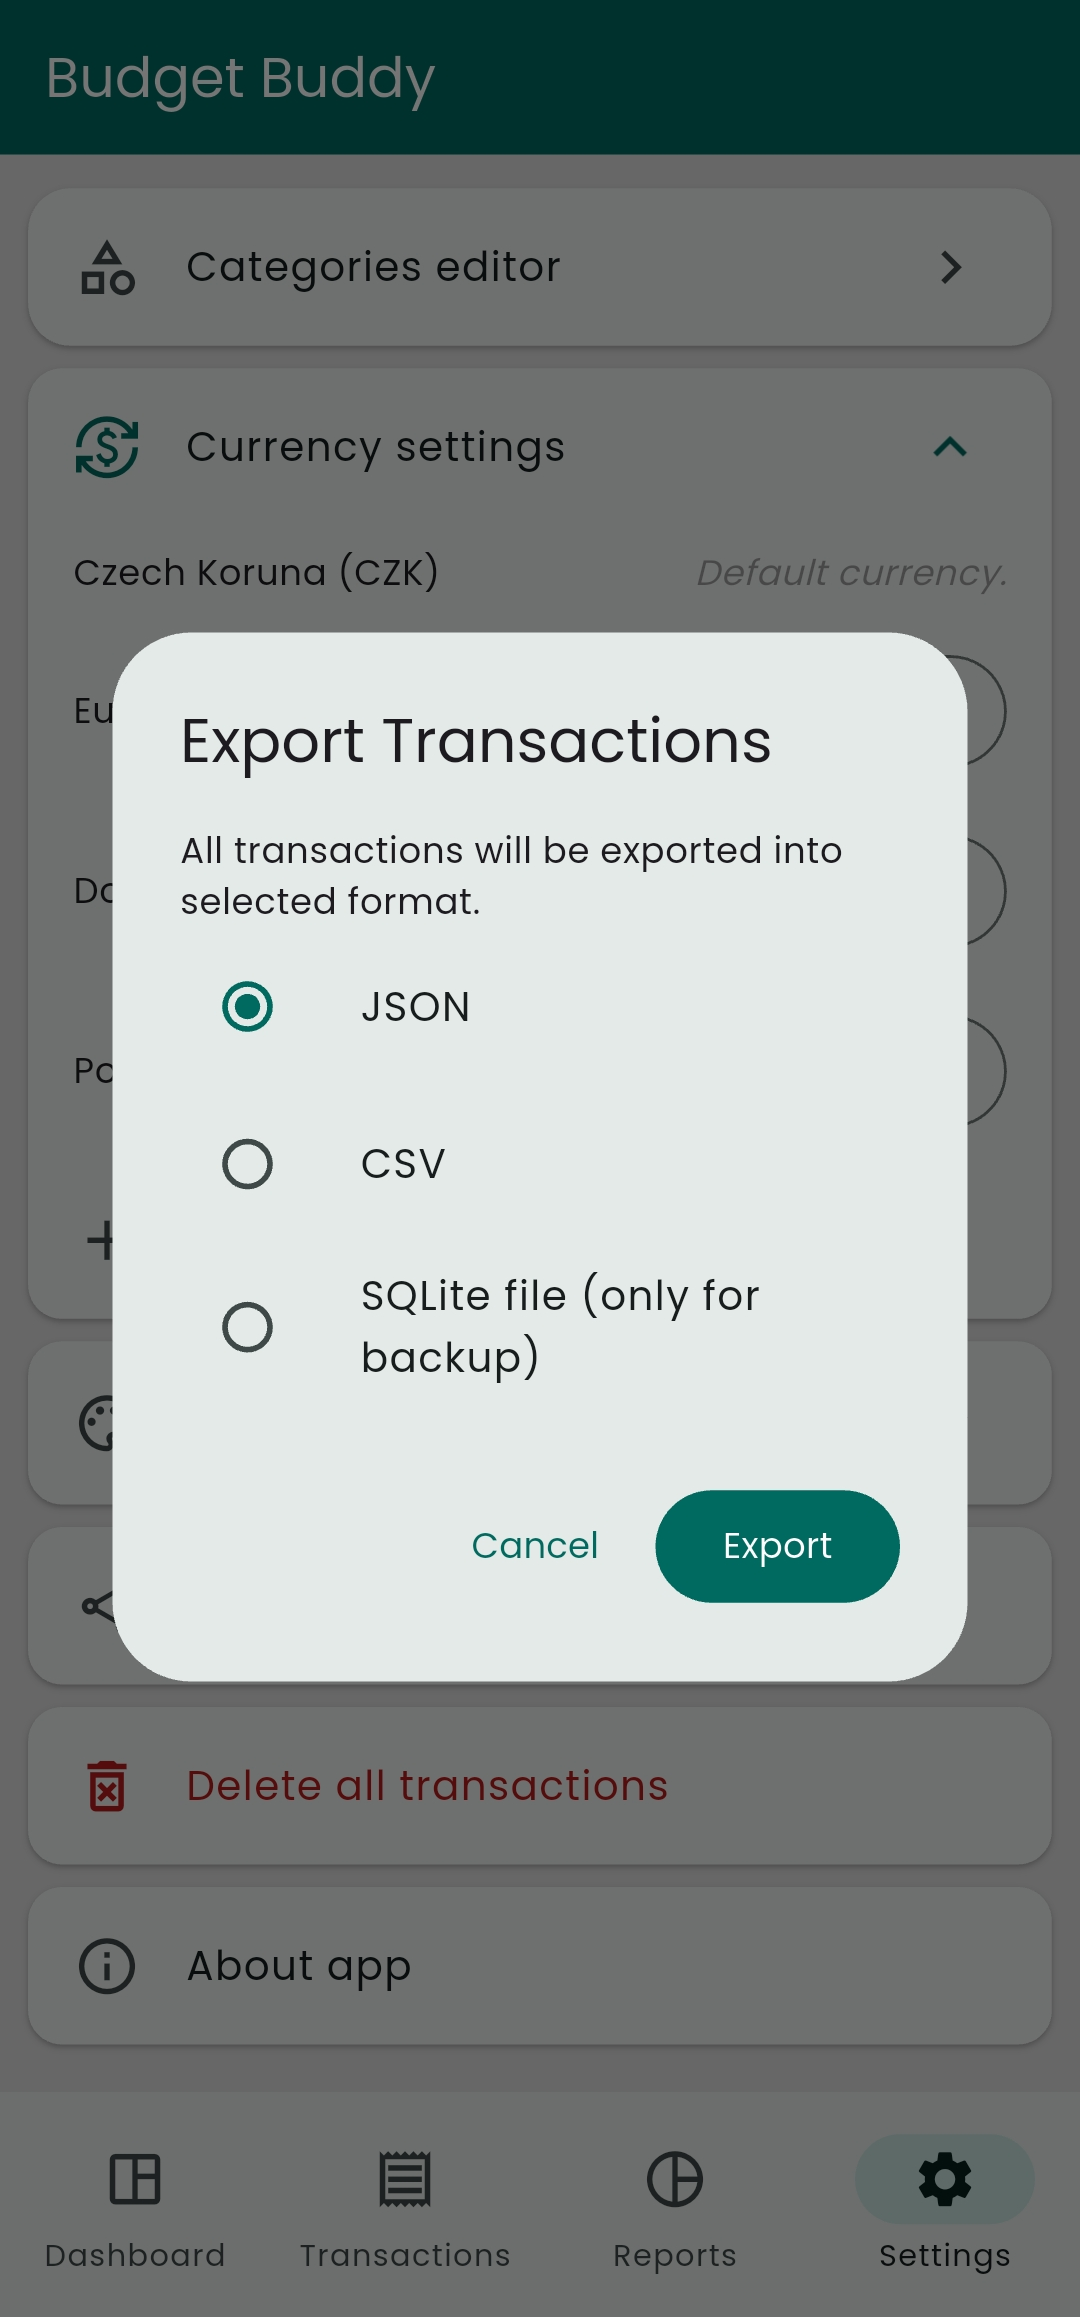
\includegraphics[width=0.45\textwidth]{images/export-mobile.png}
  \caption{Dialogové okno pro export dat na mobilním telefonu}
  \label{fig:export}
\end{figure}

\section{Možná rozšíření aplikace}
Osobně si myslím, že se nikdy nedá o~softwaru prohlásit, že by nepotřeboval vývoj a není možné mu dodat vylepšení. Už vzhledem k~vývoji technologií a~proměně uživatelských požadavků je nutné aplikaci udržovat aktuální. Se změnou požadavků se pojí rozšíření o~nové funkce a nebo naopak odstranění funkcí nepoužívaných.

\begin{enumerate}
  \item \textbf{Možnost založit více účtů} nabízí většina existujících řešení, proto se z~mého pohledu jedná o~logický krok. Tento krok by umožnil uživateli si oddělit různé účty, případně si je libovolně organizovat. Na druhou stranu se jedná o~další potenciální komplikaci pro uživatele a bylo by nutné zajistit vhodné přepínání účtů i správné zobrazení momentálně zvoleného účtu.
  \item \textbf{Překlad aplikace do jiných jazyků} umožní zpřístupnění pro uživatele ze zahraničí. Překlad aplikace není z~technického hlediska náročný a je možné ho provádět postupně. Samotné přeložení výrazů je za pomocí překladačů postavených na velkých jazykových modelech snadnou a levnou zálěžitostí.
  \item \textbf{Import dat z~jiných aplikací} je funkcionalitou, která může přimět uživatele k~přechodu na tuto aplikaci. Většina aplikací pro správu financí nabízí export dat do CSV nebo JSON formátu. I~když různé aplikace mají odlišné struktury dat, pro nejběžnější aplikace by bylo možné vytvořit konkrétní proces importu.
  \item \textbf{Umožnit výběr hlavní měny} namísto momentální pevně zvolené České koruny. Aplikace nyní kvůli sjednocení transakcí v~zahraničních měnách používá Českou korunu. Možnost volby této hlavní měny by vyžadovala změny v~logice aplikace i databázi, ale byla by realizovatelná v~rámci rozumných mezí. Tento krok by dával smysl při překladu aplikace.
\end{enumerate}

\begin{kiconclusions}
Vyvinutá multiplatformní aplikace Budget Buddy umožňuje jednoduchou správu osobních financí. Snažil jsem se o~vylepšení nedostatků existujících aplikací a zjednodušení celého procesu pro uživatele. Multiplatformnost dává uživateli možnost zvolit si oblíbené zařízení pro užívání. Použití systému Material Design jinde než na domovské platformně Android považuji za korektní, jelikož aplikace od společnosti Google jsou velmi rozšířené a tento systém užívají na různých platformách.

Pro nasazení aplikace do produkce by bylo vhodné umožnit synchronizaci dat mezi zařízeními skrz server. Tím by se vyřešil problém s~přístupem k~datům na různých zařízeních. Tento krok by vyžadoval i zavedení uživatelských účtů a přihlášení.
\end{kiconclusions}

\begin{kiconclusions}[english]
The developed cross-platform application, Budget Buddy, allows for easy management of personal finances. I~aimed to improve the shortcomings of existing applications and simplify the entire process for the user. Cross-platform support gives the user the ability to choose their preferred device for use. The use of the Material Design system on platforms other than the home Android platform Android is considered appropriate, as Google’s applications are widely used across different platforms and utilize this system.

For deployment of the application to production, it would be advisable to enable data synchronization between devices through a server. This would solve the issue of accessing data across different devices. This step would also require the introduction of user accounts and login functionality.
\end{kiconclusions}

\appendix
\section{Obsah elektronický dat} \label{sec:ObsahElData}
Součástí textu práce jsou i elektronická data v~systému Katedy informatiky PřF v~Olomouci s~touto strukturou:

\begin{description}

  \item[\texttt{src/}] \hfill \\
    Adresář obsahující soubory pro instalaci na platformy Android a Windows.
  \item[\texttt{bin/}] \hfill \\
    Adresář obsahující veškeré soubory a adresáře (v~ZIP archivu) nutné pro sestavení spustitelných souborů. Jde o~celý Flutter projekt.
  \item[\texttt{text/}] \hfill \\
    Adresář s~textem práce ve formátu PDF, vytvořený s~použitím
    závazného stylu KI PřF UP v~Olomouci pro závěrečné práce, včetně
    všech (textových) příloh, a~všechny soubory potřebné pro
    bezproblémové vytvoření PDF dokumentu textu (případně v~ZIP
    archivu), tj.~zdrojový text textu a příloh, vložené obrázky, apod.
  \item[\texttt{README.md}] \hfill \\
    Textový soubor ve značkovacím jazyku Markdown s~instrukcemi pro instalaci a spuštění aplikace.

\end{description}

% ----- tady začíná to co v práci bylo dáno

%%%  Po přeložení programem CSLaTeX (třikrát) je potřeba použít
%%%  program DVIPS a takto získaný PostScriptový soubor vytisknout
%%%  na PostScriptové tiskárně nebo pomocí programu GhostScript.
%%%
%%%  Rovněž je možné použít program DVIPDFM a vytvořit z dokumentu
%%%  soubor ve formátu PDF včetně hypertextových odkazů.

%%% Argument `joinlists' způsobí zřetězení seznamů obrázků, tabulek,
%%% vět a zdrojových kódů. Není-li použít, všechny seznamy jsou
%%% uvedeny na samostatných stránkách.

%%  'encoding=kódování' pro kódování tohoto a vložených zdrojových
%%  textů v kódování jiném než výchozím utf8

%% -------------------------------------------------------------------

%% Sazba povinné bibliografie, za přílohami (případně i za seznamem
%% zkratek). Při použití BibLaTeXu použijte makro
%% \printbibliography. jinak prostředí thebibliography. Ne obojí!

%% Sazba i v textu necitovaných zdrojů, při použití
%% BibLaTeXu. Volitelné.
%% \nocite{*}
%% Vlastní sazba bibliografie při použití BibLaTeXu.

\printbibliography

%% Sazba volitelného rejstříku, za bibliografií.
%% \printindex
%% \printglossaries
\end{document}
